\documentclass[twoside]{article}

% Packages required by doxygen
\usepackage{calc}
\usepackage{doxygen}
\usepackage{graphicx}
\usepackage[utf8]{inputenc}
\usepackage{makeidx}
\usepackage{multicol}
\usepackage{multirow}
\usepackage{textcomp}
\usepackage[table]{xcolor}

% NLS support packages
\usepackage{polski}
\usepackage[T1]{fontenc}

% Font selection
\usepackage[T1]{fontenc}
\usepackage{mathptmx}
\usepackage[scaled=.90]{helvet}
\usepackage{courier}
\usepackage{amssymb}
\usepackage{sectsty}
\renewcommand{\familydefault}{\sfdefault}
\allsectionsfont{%
  \fontseries{bc}\selectfont%
  \color{darkgray}%
}
\renewcommand{\DoxyLabelFont}{%
  \fontseries{bc}\selectfont%
  \color{darkgray}%
}

% Page & text layout
\usepackage{geometry}
\geometry{%
  a4paper,%
  top=2.5cm,%
  bottom=2.5cm,%
  left=2.5cm,%
  right=2.5cm%
}
\tolerance=750
\hfuzz=15pt
\hbadness=750
\setlength{\emergencystretch}{15pt}
\setlength{\parindent}{0cm}
\setlength{\parskip}{0.2cm}
\makeatletter
\renewcommand{\paragraph}{%
  \@startsection{paragraph}{4}{0ex}{-1.0ex}{1.0ex}{%
    \normalfont\normalsize\bfseries\SS@parafont%
  }%
}
\renewcommand{\subparagraph}{%
  \@startsection{subparagraph}{5}{0ex}{-1.0ex}{1.0ex}{%
    \normalfont\normalsize\bfseries\SS@subparafont%
  }%
}
\makeatother

% Headers & footers
\usepackage{fancyhdr}
\pagestyle{fancyplain}
\fancyhead[LE]{\fancyplain{}{\bfseries\thepage}}
\fancyhead[CE]{\fancyplain{}{}}
\fancyhead[RE]{\fancyplain{}{\bfseries\leftmark}}
\fancyhead[LO]{\fancyplain{}{\bfseries\rightmark}}
\fancyhead[CO]{\fancyplain{}{}}
\fancyhead[RO]{\fancyplain{}{\bfseries\thepage}}
\fancyfoot[LE]{\fancyplain{}{}}
\fancyfoot[CE]{\fancyplain{}{}}
\fancyfoot[RE]{\fancyplain{}{\bfseries\scriptsize Wygenerowano Pt, 6 maj 2016 21\-:34\-:04 dla Graf programem Doxygen }}
\fancyfoot[LO]{\fancyplain{}{\bfseries\scriptsize Wygenerowano Pt, 6 maj 2016 21\-:34\-:04 dla Graf programem Doxygen }}
\fancyfoot[CO]{\fancyplain{}{}}
\fancyfoot[RO]{\fancyplain{}{}}
\renewcommand{\footrulewidth}{0.4pt}
\renewcommand{\sectionmark}[1]{%
  \markright{\thesection\ #1}%
}

% Indices & bibliography
\usepackage{natbib}
\usepackage[titles]{tocloft}
\setcounter{tocdepth}{3}
\setcounter{secnumdepth}{5}
\makeindex

% Hyperlinks (required, but should be loaded last)
\usepackage{ifpdf}
\ifpdf
  \usepackage[pdftex,pagebackref=true]{hyperref}
\else
  \usepackage[ps2pdf,pagebackref=true]{hyperref}
\fi
\hypersetup{%
  colorlinks=true,%
  linkcolor=blue,%
  citecolor=blue,%
  unicode%
}

% Custom commands
\newcommand{\clearemptydoublepage}{%
  \newpage{\pagestyle{empty}\cleardoublepage}%
}


%===== C O N T E N T S =====

\begin{document}

% Titlepage & ToC
\hypersetup{pageanchor=false}
\pagenumbering{roman}
\begin{titlepage}
\vspace*{7cm}
\begin{center}%
{\Large Graf }\\
\vspace*{1cm}
{\large Wygenerowano przez Doxygen 1.8.6}\\
\vspace*{0.5cm}
{\small Pt, 6 maj 2016 21:34:04}\\
\end{center}
\end{titlepage}
\tableofcontents
\pagenumbering{arabic}
\hypersetup{pageanchor=true}

%--- Begin generated contents ---
\section{Indeks hierarchiczny}
\subsection{Hierarchia klas}
Ta lista dziedziczenia posortowana jest z grubsza, choć nie całkowicie, alfabetycznie\-:\begin{DoxyCompactList}
\item \contentsline{section}{B\-Node$<$ Object $>$}{\pageref{class_b_node}}{}
\item \contentsline{section}{B\-Node$<$ unsigned $>$}{\pageref{class_b_node}}{}
\item \contentsline{section}{I\-Graph}{\pageref{class_i_graph}}{}
\begin{DoxyCompactList}
\item \contentsline{section}{Graph}{\pageref{class_graph}}{}
\begin{DoxyCompactList}
\item \contentsline{section}{Graph\-\_\-\-Test$<$ Object $>$}{\pageref{class_graph___test}}{}
\end{DoxyCompactList}
\end{DoxyCompactList}
\item \contentsline{section}{I\-List$<$ Object $>$}{\pageref{class_i_list}}{}
\begin{DoxyCompactList}
\item \contentsline{section}{B\-List$<$ Object $>$}{\pageref{class_b_list}}{}
\end{DoxyCompactList}
\item \contentsline{section}{I\-List$<$ unsigned $>$}{\pageref{class_i_list}}{}
\begin{DoxyCompactList}
\item \contentsline{section}{B\-List$<$ unsigned $>$}{\pageref{class_b_list}}{}
\end{DoxyCompactList}
\item \contentsline{section}{I\-Queue$<$ Object $>$}{\pageref{class_i_queue}}{}
\begin{DoxyCompactList}
\item \contentsline{section}{Kolejka$<$ Object $>$}{\pageref{class_kolejka}}{}
\end{DoxyCompactList}
\item \contentsline{section}{I\-Runnable$<$ Object $>$}{\pageref{class_i_runnable}}{}
\begin{DoxyCompactList}
\item \contentsline{section}{Graph\-\_\-\-Test$<$ Object $>$}{\pageref{class_graph___test}}{}
\end{DoxyCompactList}
\item \contentsline{section}{I\-Stack$<$ Object $>$}{\pageref{class_i_stack}}{}
\begin{DoxyCompactList}
\item \contentsline{section}{Stos$<$ Object $>$}{\pageref{class_stos}}{}
\end{DoxyCompactList}
\item \contentsline{section}{S\-Node$<$ Object $>$}{\pageref{class_s_node}}{}
\item \contentsline{section}{Stopwatch}{\pageref{class_stopwatch}}{}
\begin{DoxyCompactList}
\item \contentsline{section}{Advanced\-Stopwatch}{\pageref{class_advanced_stopwatch}}{}
\end{DoxyCompactList}
\end{DoxyCompactList}

\section{Indeks klas}
\subsection{Lista klas}
Tutaj znajdują się klasy, struktury, unie i interfejsy wraz z ich krótkimi opisami\-:\begin{DoxyCompactList}
\item\contentsline{section}{\hyperlink{class_advanced_stopwatch}{Advanced\-Stopwatch} \\*Klasa implementująca rozbudowany stoper }{\pageref{class_advanced_stopwatch}}{}
\item\contentsline{section}{\hyperlink{class_b_list}{B\-List$<$ Object $>$} \\*Szablonowa klasa implementująca listę dwukierunkową }{\pageref{class_b_list}}{}
\item\contentsline{section}{\hyperlink{class_b_node}{B\-Node$<$ Object $>$} }{\pageref{class_b_node}}{}
\item\contentsline{section}{\hyperlink{class_graph}{Graph} }{\pageref{class_graph}}{}
\item\contentsline{section}{\hyperlink{class_graph___test}{Graph\-\_\-\-Test$<$ Object $>$} \\*Szablonowa klasa implementująca testowy graf }{\pageref{class_graph___test}}{}
\item\contentsline{section}{\hyperlink{class_i_graph}{I\-Graph} }{\pageref{class_i_graph}}{}
\item\contentsline{section}{\hyperlink{class_i_list}{I\-List$<$ Object $>$} \\*Interfejs listy dwukierunkowej }{\pageref{class_i_list}}{}
\item\contentsline{section}{\hyperlink{class_i_queue}{I\-Queue$<$ Object $>$} \\*Klasa modelująca interfejs kolejki }{\pageref{class_i_queue}}{}
\item\contentsline{section}{\hyperlink{class_i_runnable}{I\-Runnable$<$ Object $>$} \\*Klasa szablonowa modelująca interfejs \char`\"{}\-Biegacza\char`\"{} }{\pageref{class_i_runnable}}{}
\item\contentsline{section}{\hyperlink{class_i_stack}{I\-Stack$<$ Object $>$} \\*Klasa szablonowa modelująca interfejs stosu }{\pageref{class_i_stack}}{}
\item\contentsline{section}{\hyperlink{class_kolejka}{Kolejka$<$ Object $>$} \\*Klasa szablonowa implementująca kolejkę }{\pageref{class_kolejka}}{}
\item\contentsline{section}{\hyperlink{class_s_node}{S\-Node$<$ Object $>$} }{\pageref{class_s_node}}{}
\item\contentsline{section}{\hyperlink{class_stopwatch}{Stopwatch} \\*Klasa implementująca podstawowy stoper }{\pageref{class_stopwatch}}{}
\item\contentsline{section}{\hyperlink{class_stos}{Stos$<$ Object $>$} \\*Klasa szablonowa implementująca stos }{\pageref{class_stos}}{}
\end{DoxyCompactList}

\section{Indeks plików}
\subsection{Lista plików}
Tutaj znajduje się lista wszystkich plików z ich krótkimi opisami\-:\begin{DoxyCompactList}
\item\contentsline{section}{prj/inc/\hyperlink{_advanced_stopwatch_8hh}{Advanced\-Stopwatch.\-hh} }{\pageref{_advanced_stopwatch_8hh}}{}
\item\contentsline{section}{prj/inc/\hyperlink{_b_list_8hh}{B\-List.\-hh} }{\pageref{_b_list_8hh}}{}
\item\contentsline{section}{prj/inc/\hyperlink{_b_node_8hh}{B\-Node.\-hh} }{\pageref{_b_node_8hh}}{}
\item\contentsline{section}{prj/inc/\hyperlink{_graph_8hh}{Graph.\-hh} }{\pageref{_graph_8hh}}{}
\item\contentsline{section}{prj/inc/\hyperlink{_graph___test_8hh}{Graph\-\_\-\-Test.\-hh} }{\pageref{_graph___test_8hh}}{}
\item\contentsline{section}{prj/inc/\hyperlink{_i_graph_8hh}{I\-Graph.\-hh} }{\pageref{_i_graph_8hh}}{}
\item\contentsline{section}{prj/inc/\hyperlink{_i_list_8hh}{I\-List.\-hh} }{\pageref{_i_list_8hh}}{}
\item\contentsline{section}{prj/inc/\hyperlink{_i_queue_8hh}{I\-Queue.\-hh} }{\pageref{_i_queue_8hh}}{}
\item\contentsline{section}{prj/inc/\hyperlink{_i_runnable_8hh}{I\-Runnable.\-hh} }{\pageref{_i_runnable_8hh}}{}
\item\contentsline{section}{prj/inc/\hyperlink{_i_stack_8hh}{I\-Stack.\-hh} }{\pageref{_i_stack_8hh}}{}
\item\contentsline{section}{prj/inc/\hyperlink{_kolejka_8hh}{Kolejka.\-hh} }{\pageref{_kolejka_8hh}}{}
\item\contentsline{section}{prj/inc/\hyperlink{_s_node_8hh}{S\-Node.\-hh} }{\pageref{_s_node_8hh}}{}
\item\contentsline{section}{prj/inc/\hyperlink{_stopwatch_8hh}{Stopwatch.\-hh} }{\pageref{_stopwatch_8hh}}{}
\item\contentsline{section}{prj/inc/\hyperlink{_stos_8hh}{Stos.\-hh} }{\pageref{_stos_8hh}}{}
\item\contentsline{section}{prj/src/\hyperlink{_advanced_stopwatch_8cpp}{Advanced\-Stopwatch.\-cpp} }{\pageref{_advanced_stopwatch_8cpp}}{}
\item\contentsline{section}{prj/src/\hyperlink{_graph_8cpp}{Graph.\-cpp} }{\pageref{_graph_8cpp}}{}
\item\contentsline{section}{prj/src/\hyperlink{main_8cpp}{main.\-cpp} }{\pageref{main_8cpp}}{}
\item\contentsline{section}{prj/src/\hyperlink{_stopwatch_8cpp}{Stopwatch.\-cpp} }{\pageref{_stopwatch_8cpp}}{}
\end{DoxyCompactList}

\section{Dokumentacja klas}
\hypertarget{class_advanced_stopwatch}{\subsection{Dokumentacja klasy Advanced\-Stopwatch}
\label{class_advanced_stopwatch}\index{Advanced\-Stopwatch@{Advanced\-Stopwatch}}
}


Klasa implementująca rozbudowany stoper.  




{\ttfamily \#include $<$Advanced\-Stopwatch.\-hh$>$}



Diagram dziedziczenia dla Advanced\-Stopwatch
\nopagebreak
\begin{figure}[H]
\begin{center}
\leavevmode
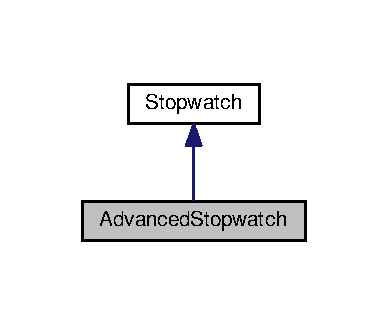
\includegraphics[width=186pt]{class_advanced_stopwatch__inherit__graph}
\end{center}
\end{figure}


Diagram współpracy dla Advanced\-Stopwatch\-:
\nopagebreak
\begin{figure}[H]
\begin{center}
\leavevmode
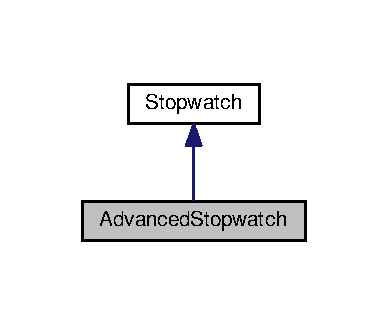
\includegraphics[width=186pt]{class_advanced_stopwatch__coll__graph}
\end{center}
\end{figure}
\subsubsection*{Metody publiczne}
\begin{DoxyCompactItemize}
\item 
\hyperlink{class_advanced_stopwatch_a2b43f9deab93398578e31205038d4f23}{Advanced\-Stopwatch} ()
\item 
\hyperlink{class_advanced_stopwatch_ab7f73fdeabf44c1557f27c6542099cd5}{$\sim$\-Advanced\-Stopwatch} ()
\item 
unsigned \& \hyperlink{class_advanced_stopwatch_ae4c7ec4341d3e7db1d75b704d1c75030}{Rozmiar} ()
\item 
bool \hyperlink{class_advanced_stopwatch_ad59c3b0557fc23c1cba33964259a6113}{Save\-Elapsed\-Time} (double rekord)
\begin{DoxyCompactList}\small\item\em Metoda zapisująca wartość pomiaru czasu okrążenia. \end{DoxyCompactList}\item 
double \hyperlink{class_advanced_stopwatch_a12a5049b736e3e394361f57221224b7e}{Series\-Average} ()
\begin{DoxyCompactList}\small\item\em Metoda wyliczająca średni czas okrążenia. \end{DoxyCompactList}\item 
bool \hyperlink{class_advanced_stopwatch_a559af3abdf7adbae5ef03f5d58b1b49c}{Save\-Average\-Time\-To\-Buffer} (double rekord)
\begin{DoxyCompactList}\small\item\em Metoda zapisująca średni czas okrążenia do bufora plikowego. \end{DoxyCompactList}\item 
void \hyperlink{class_advanced_stopwatch_ad05cc1b4240cd225ee92bec0d02cd6fd}{Print\-Elapsed\-Times} ()
\begin{DoxyCompactList}\small\item\em Metoda wypisująca zawartość pamięci stopera. \end{DoxyCompactList}\item 
void \hyperlink{class_advanced_stopwatch_a918c9a7a39e8984281e8dd531473183e}{Clean\-Elapsed\-Times} ()
\begin{DoxyCompactList}\small\item\em Metoda usuwająca zawartość pamięci stopera. \end{DoxyCompactList}\item 
void \hyperlink{class_advanced_stopwatch_a71d86e77bbd4e7e92da83a7e177b0925}{Clean\-File\-Buffer} ()
\begin{DoxyCompactList}\small\item\em Metoda usuwająca zawartość bufora plikowego stopera. \end{DoxyCompactList}\item 
bool \hyperlink{class_advanced_stopwatch_a36ceb90b161eccfbaecea8c193934d43}{Dump\-File\-Buffer} (string nazwa\-Pliku)
\begin{DoxyCompactList}\small\item\em Metoda zapisująca zawartość bufora plikowego do pliku. \end{DoxyCompactList}\item 
bool \hyperlink{class_advanced_stopwatch_a62b8dcebc84f7c35e742de1ca857f397}{Dump\-To\-File} (string nazwa\-Pliku, double rekord)
\begin{DoxyCompactList}\small\item\em Metoda zapisująca pojedynczy rekord bufora plikowego do pliku. \end{DoxyCompactList}\end{DoxyCompactItemize}
\subsubsection*{Dodatkowe Dziedziczone Składowe}


\subsubsection{Opis szczegółowy}
Klasa implementująca rozbudowany stoper. 

Klasa jest modelelem stopera z funkcją zapisu czasu okrążeń, liczeniem średniego czasu kilku okrążeń, zapisu zmierzonych czasów do pliku. 

Definicja w linii 28 pliku Advanced\-Stopwatch.\-hh.



\subsubsection{Dokumentacja konstruktora i destruktora}
\hypertarget{class_advanced_stopwatch_a2b43f9deab93398578e31205038d4f23}{\index{Advanced\-Stopwatch@{Advanced\-Stopwatch}!Advanced\-Stopwatch@{Advanced\-Stopwatch}}
\index{Advanced\-Stopwatch@{Advanced\-Stopwatch}!AdvancedStopwatch@{Advanced\-Stopwatch}}
\paragraph[{Advanced\-Stopwatch}]{\setlength{\rightskip}{0pt plus 5cm}Advanced\-Stopwatch\-::\-Advanced\-Stopwatch (
\begin{DoxyParamCaption}
{}
\end{DoxyParamCaption}
)}}\label{class_advanced_stopwatch_a2b43f9deab93398578e31205038d4f23}


Definicja w linii 4 pliku Advanced\-Stopwatch.\-cpp.

\hypertarget{class_advanced_stopwatch_ab7f73fdeabf44c1557f27c6542099cd5}{\index{Advanced\-Stopwatch@{Advanced\-Stopwatch}!$\sim$\-Advanced\-Stopwatch@{$\sim$\-Advanced\-Stopwatch}}
\index{$\sim$\-Advanced\-Stopwatch@{$\sim$\-Advanced\-Stopwatch}!AdvancedStopwatch@{Advanced\-Stopwatch}}
\paragraph[{$\sim$\-Advanced\-Stopwatch}]{\setlength{\rightskip}{0pt plus 5cm}Advanced\-Stopwatch\-::$\sim$\-Advanced\-Stopwatch (
\begin{DoxyParamCaption}
{}
\end{DoxyParamCaption}
)}}\label{class_advanced_stopwatch_ab7f73fdeabf44c1557f27c6542099cd5}


Definicja w linii 15 pliku Advanced\-Stopwatch.\-cpp.



\subsubsection{Dokumentacja funkcji składowych}
\hypertarget{class_advanced_stopwatch_a918c9a7a39e8984281e8dd531473183e}{\index{Advanced\-Stopwatch@{Advanced\-Stopwatch}!Clean\-Elapsed\-Times@{Clean\-Elapsed\-Times}}
\index{Clean\-Elapsed\-Times@{Clean\-Elapsed\-Times}!AdvancedStopwatch@{Advanced\-Stopwatch}}
\paragraph[{Clean\-Elapsed\-Times}]{\setlength{\rightskip}{0pt plus 5cm}void Advanced\-Stopwatch\-::\-Clean\-Elapsed\-Times (
\begin{DoxyParamCaption}
{}
\end{DoxyParamCaption}
)}}\label{class_advanced_stopwatch_a918c9a7a39e8984281e8dd531473183e}


Metoda usuwająca zawartość pamięci stopera. 



Definicja w linii 66 pliku Advanced\-Stopwatch.\-cpp.

\hypertarget{class_advanced_stopwatch_a71d86e77bbd4e7e92da83a7e177b0925}{\index{Advanced\-Stopwatch@{Advanced\-Stopwatch}!Clean\-File\-Buffer@{Clean\-File\-Buffer}}
\index{Clean\-File\-Buffer@{Clean\-File\-Buffer}!AdvancedStopwatch@{Advanced\-Stopwatch}}
\paragraph[{Clean\-File\-Buffer}]{\setlength{\rightskip}{0pt plus 5cm}void Advanced\-Stopwatch\-::\-Clean\-File\-Buffer (
\begin{DoxyParamCaption}
{}
\end{DoxyParamCaption}
)}}\label{class_advanced_stopwatch_a71d86e77bbd4e7e92da83a7e177b0925}


Metoda usuwająca zawartość bufora plikowego stopera. 



Definicja w linii 74 pliku Advanced\-Stopwatch.\-cpp.

\hypertarget{class_advanced_stopwatch_a36ceb90b161eccfbaecea8c193934d43}{\index{Advanced\-Stopwatch@{Advanced\-Stopwatch}!Dump\-File\-Buffer@{Dump\-File\-Buffer}}
\index{Dump\-File\-Buffer@{Dump\-File\-Buffer}!AdvancedStopwatch@{Advanced\-Stopwatch}}
\paragraph[{Dump\-File\-Buffer}]{\setlength{\rightskip}{0pt plus 5cm}bool Advanced\-Stopwatch\-::\-Dump\-File\-Buffer (
\begin{DoxyParamCaption}
\item[{string}]{nazwa\-Pliku}
\end{DoxyParamCaption}
)}}\label{class_advanced_stopwatch_a36ceb90b161eccfbaecea8c193934d43}


Metoda zapisująca zawartość bufora plikowego do pliku. 

Dokonuje zapisu rekordów w buforze do pliku. 
\begin{DoxyParams}[1]{Parametry}
\mbox{\tt in}  & {\em nazwa\-Pliku} & -\/ nazwa pliku, do którego mają zostać zapisane czasy \\
\hline
\end{DoxyParams}

\begin{DoxyRetVals}{Zwracane wartości}
{\em true} & -\/ jeśli udało się zapisać \\
\hline
{\em false} & -\/ jeśli udało się zapisać \\
\hline
\end{DoxyRetVals}


Definicja w linii 80 pliku Advanced\-Stopwatch.\-cpp.

\hypertarget{class_advanced_stopwatch_a62b8dcebc84f7c35e742de1ca857f397}{\index{Advanced\-Stopwatch@{Advanced\-Stopwatch}!Dump\-To\-File@{Dump\-To\-File}}
\index{Dump\-To\-File@{Dump\-To\-File}!AdvancedStopwatch@{Advanced\-Stopwatch}}
\paragraph[{Dump\-To\-File}]{\setlength{\rightskip}{0pt plus 5cm}bool Advanced\-Stopwatch\-::\-Dump\-To\-File (
\begin{DoxyParamCaption}
\item[{string}]{nazwa\-Pliku, }
\item[{double}]{rekord}
\end{DoxyParamCaption}
)}}\label{class_advanced_stopwatch_a62b8dcebc84f7c35e742de1ca857f397}


Metoda zapisująca pojedynczy rekord bufora plikowego do pliku. 

Dokonuje zapisu wybranego rekordu w buforze do pliku. 
\begin{DoxyParams}[1]{Parametry}
\mbox{\tt in}  & {\em nazwa\-Pliku} & -\/ nazwa pliku, do którego ma zostać zapisany czas \\
\hline
\mbox{\tt in}  & {\em rekord} & -\/ wartość pomiaru czasu, która ma być zapisana \\
\hline
\end{DoxyParams}

\begin{DoxyRetVals}{Zwracane wartości}
{\em true} & -\/ jeśli udało się zapisać \\
\hline
{\em false} & -\/ jeśli udało się zapisać \\
\hline
\end{DoxyRetVals}


Definicja w linii 98 pliku Advanced\-Stopwatch.\-cpp.

\hypertarget{class_advanced_stopwatch_ad05cc1b4240cd225ee92bec0d02cd6fd}{\index{Advanced\-Stopwatch@{Advanced\-Stopwatch}!Print\-Elapsed\-Times@{Print\-Elapsed\-Times}}
\index{Print\-Elapsed\-Times@{Print\-Elapsed\-Times}!AdvancedStopwatch@{Advanced\-Stopwatch}}
\paragraph[{Print\-Elapsed\-Times}]{\setlength{\rightskip}{0pt plus 5cm}void Advanced\-Stopwatch\-::\-Print\-Elapsed\-Times (
\begin{DoxyParamCaption}
{}
\end{DoxyParamCaption}
)}}\label{class_advanced_stopwatch_ad05cc1b4240cd225ee92bec0d02cd6fd}


Metoda wypisująca zawartość pamięci stopera. 



Definicja w linii 58 pliku Advanced\-Stopwatch.\-cpp.

\hypertarget{class_advanced_stopwatch_ae4c7ec4341d3e7db1d75b704d1c75030}{\index{Advanced\-Stopwatch@{Advanced\-Stopwatch}!Rozmiar@{Rozmiar}}
\index{Rozmiar@{Rozmiar}!AdvancedStopwatch@{Advanced\-Stopwatch}}
\paragraph[{Rozmiar}]{\setlength{\rightskip}{0pt plus 5cm}unsigned\& Advanced\-Stopwatch\-::\-Rozmiar (
\begin{DoxyParamCaption}
{}
\end{DoxyParamCaption}
)\hspace{0.3cm}{\ttfamily [inline]}}}\label{class_advanced_stopwatch_ae4c7ec4341d3e7db1d75b704d1c75030}


Definicja w linii 36 pliku Advanced\-Stopwatch.\-hh.

\hypertarget{class_advanced_stopwatch_a559af3abdf7adbae5ef03f5d58b1b49c}{\index{Advanced\-Stopwatch@{Advanced\-Stopwatch}!Save\-Average\-Time\-To\-Buffer@{Save\-Average\-Time\-To\-Buffer}}
\index{Save\-Average\-Time\-To\-Buffer@{Save\-Average\-Time\-To\-Buffer}!AdvancedStopwatch@{Advanced\-Stopwatch}}
\paragraph[{Save\-Average\-Time\-To\-Buffer}]{\setlength{\rightskip}{0pt plus 5cm}bool Advanced\-Stopwatch\-::\-Save\-Average\-Time\-To\-Buffer (
\begin{DoxyParamCaption}
\item[{double}]{rekord}
\end{DoxyParamCaption}
)}}\label{class_advanced_stopwatch_a559af3abdf7adbae5ef03f5d58b1b49c}


Metoda zapisująca średni czas okrążenia do bufora plikowego. 

Dodaje podany czas do pamięci stopera, z której można dokonać zapisu do pliku. 
\begin{DoxyParams}[1]{Parametry}
\mbox{\tt in}  & {\em rekord} & -\/ wartość pomiaru czasu \\
\hline
\end{DoxyParams}

\begin{DoxyRetVals}{Zwracane wartości}
{\em true} & -\/ jeśli udało się zapisać \\
\hline
{\em false} & -\/ jeśli udało się zapisać \\
\hline
\end{DoxyRetVals}


Definicja w linii 49 pliku Advanced\-Stopwatch.\-cpp.

\hypertarget{class_advanced_stopwatch_ad59c3b0557fc23c1cba33964259a6113}{\index{Advanced\-Stopwatch@{Advanced\-Stopwatch}!Save\-Elapsed\-Time@{Save\-Elapsed\-Time}}
\index{Save\-Elapsed\-Time@{Save\-Elapsed\-Time}!AdvancedStopwatch@{Advanced\-Stopwatch}}
\paragraph[{Save\-Elapsed\-Time}]{\setlength{\rightskip}{0pt plus 5cm}bool Advanced\-Stopwatch\-::\-Save\-Elapsed\-Time (
\begin{DoxyParamCaption}
\item[{double}]{rekord}
\end{DoxyParamCaption}
)}}\label{class_advanced_stopwatch_ad59c3b0557fc23c1cba33964259a6113}


Metoda zapisująca wartość pomiaru czasu okrążenia. 

Dodaje podany czas do tablicy czasów okrążeń. 
\begin{DoxyParams}[1]{Parametry}
\mbox{\tt in}  & {\em rekord} & -\/ wartość pomiaru czasu \\
\hline
\end{DoxyParams}

\begin{DoxyRetVals}{Zwracane wartości}
{\em true} & -\/ jeśli udało się zapisać \\
\hline
{\em false} & -\/ jeśli udało się zapisać \\
\hline
\end{DoxyRetVals}


Definicja w linii 26 pliku Advanced\-Stopwatch.\-cpp.

\hypertarget{class_advanced_stopwatch_a12a5049b736e3e394361f57221224b7e}{\index{Advanced\-Stopwatch@{Advanced\-Stopwatch}!Series\-Average@{Series\-Average}}
\index{Series\-Average@{Series\-Average}!AdvancedStopwatch@{Advanced\-Stopwatch}}
\paragraph[{Series\-Average}]{\setlength{\rightskip}{0pt plus 5cm}double Advanced\-Stopwatch\-::\-Series\-Average (
\begin{DoxyParamCaption}
{}
\end{DoxyParamCaption}
)}}\label{class_advanced_stopwatch_a12a5049b736e3e394361f57221224b7e}


Metoda wyliczająca średni czas okrążenia. 



Definicja w linii 37 pliku Advanced\-Stopwatch.\-cpp.



Dokumentacja dla tej klasy została wygenerowana z plików\-:\begin{DoxyCompactItemize}
\item 
prj/inc/\hyperlink{_advanced_stopwatch_8hh}{Advanced\-Stopwatch.\-hh}\item 
prj/src/\hyperlink{_advanced_stopwatch_8cpp}{Advanced\-Stopwatch.\-cpp}\end{DoxyCompactItemize}

\hypertarget{class_b_list}{\subsection{Dokumentacja szablonu klasy B\-List$<$ Object $>$}
\label{class_b_list}\index{B\-List$<$ Object $>$@{B\-List$<$ Object $>$}}
}


Szablonowa klasa implementująca listę dwukierunkową  




{\ttfamily \#include $<$B\-List.\-hh$>$}



Diagram dziedziczenia dla B\-List$<$ Object $>$
\nopagebreak
\begin{figure}[H]
\begin{center}
\leavevmode
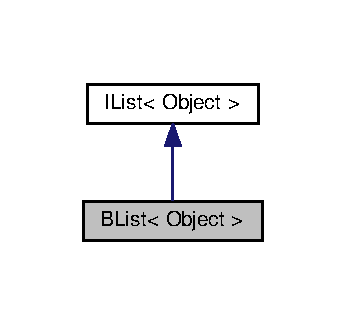
\includegraphics[width=166pt]{class_b_list__inherit__graph}
\end{center}
\end{figure}


Diagram współpracy dla B\-List$<$ Object $>$\-:
\nopagebreak
\begin{figure}[H]
\begin{center}
\leavevmode
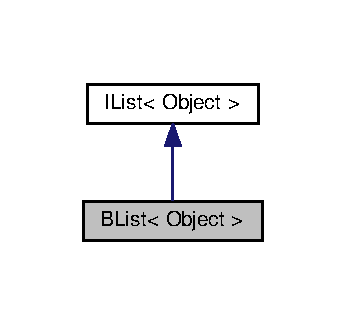
\includegraphics[width=166pt]{class_b_list__coll__graph}
\end{center}
\end{figure}
\subsubsection*{Metody publiczne}
\begin{DoxyCompactItemize}
\item 
\hyperlink{class_b_list_a5c2484087706cf974e47ea4dfb6c83ca}{B\-List} ()
\begin{DoxyCompactList}\small\item\em Konstruktor listy dwukierunkowej. \end{DoxyCompactList}\item 
\hyperlink{class_b_list_a370a72d6aece919c9cc048563077eab8}{$\sim$\-B\-List} ()
\begin{DoxyCompactList}\small\item\em Destruktor listy dwukierunkowej. \end{DoxyCompactList}\item 
\hyperlink{class_b_node}{B\-Node}$<$ Object $>$ $\ast$\& \hyperlink{class_b_list_a985da34d870b50fd254568206c6d2522}{Head} ()
\begin{DoxyCompactList}\small\item\em Metoda zwracająca głowę listy. \end{DoxyCompactList}\item 
\hyperlink{class_b_node}{B\-Node}$<$ Object $>$ $\ast$\& \hyperlink{class_b_list_a8b8f2f947c10fedf2a49cbe59f7f4d6f}{Tail} ()
\begin{DoxyCompactList}\small\item\em Metoda zwracająca ogon listy. \end{DoxyCompactList}\item 
\hyperlink{class_b_node}{B\-Node}$<$ Object $>$ $\ast$ \hyperlink{class_b_list_af7803b6789c78625383905e167fe1f3c}{Find} (Object k)
\begin{DoxyCompactList}\small\item\em Metoda wyszukująca element na liście. \end{DoxyCompactList}\item 
virtual bool \hyperlink{class_b_list_ae69bf69a67a46e5a3a0a9ba743354b2b}{Is\-Empty} ()
\begin{DoxyCompactList}\small\item\em Metoda sprawdzająca, czy lista jest pusta. \end{DoxyCompactList}\item 
virtual void \hyperlink{class_b_list_a3ce77cc9d73682bfac57c70dafdce89d}{Add\-Front} (const Object new\-Item)
\item 
virtual void \hyperlink{class_b_list_aacb4abd5a4dbe72dbf448d299eb4c6b8}{Add\-Back} (const Object new\-Item)
\item 
void \hyperlink{class_b_list_a2c602a2e303614fae5e8249146bc3966}{Add\-After} (\hyperlink{class_b_node}{B\-Node}$<$ Object $>$ $\ast$p, const Object new\-Item)
\begin{DoxyCompactList}\small\item\em Metoda dodająca element we wskazane miejsce na liście. \end{DoxyCompactList}\item 
const Object \& \hyperlink{class_b_list_ab0e7cb0e34864ec6937e281eaa48eb32}{Remove} (\hyperlink{class_b_node}{B\-Node}$<$ Object $>$ $\ast$p)
\begin{DoxyCompactList}\small\item\em Metoda usuwająca wskazany element listy. \end{DoxyCompactList}\item 
virtual const Object \& \hyperlink{class_b_list_a510b274bdcccf50699b41233a5f42a5f}{Remove\-Front} ()
\item 
virtual const Object \& \hyperlink{class_b_list_a4df7a72e29bfb324ca366fc2322184ea}{Remove\-Back} ()
\item 
void \hyperlink{class_b_list_a4382952f2329e9ec3d1403105ee26344}{Print} ()
\end{DoxyCompactItemize}


\subsubsection{Opis szczegółowy}
\subsubsection*{template$<$typename Object$>$class B\-List$<$ Object $>$}

Szablonowa klasa implementująca listę dwukierunkową 

\hyperlink{class_b_list}{B\-List} jest zbudowana w oparciu o węzły \hyperlink{class_b_node}{B\-Node} oraz operacje na wskaźnikach.

\hyperlink{class_b_list}{B\-List} może przechowywać dowolny typ danych dzięki zastosowaniu szablonu. 

Definicja w linii 25 pliku B\-List.\-hh.



\subsubsection{Dokumentacja konstruktora i destruktora}
\hypertarget{class_b_list_a5c2484087706cf974e47ea4dfb6c83ca}{\index{B\-List@{B\-List}!B\-List@{B\-List}}
\index{B\-List@{B\-List}!BList@{B\-List}}
\paragraph[{B\-List}]{\setlength{\rightskip}{0pt plus 5cm}template$<$typename Object $>$ {\bf B\-List}$<$ Object $>$\-::{\bf B\-List} (
\begin{DoxyParamCaption}
{}
\end{DoxyParamCaption}
)}}\label{class_b_list_a5c2484087706cf974e47ea4dfb6c83ca}


Konstruktor listy dwukierunkowej. 

Inicjuje listę poprzez ustawienie wskaźnika N\-U\-L\-L jako początek (head) tej listy. 

Definicja w linii 112 pliku B\-List.\-hh.

\hypertarget{class_b_list_a370a72d6aece919c9cc048563077eab8}{\index{B\-List@{B\-List}!$\sim$\-B\-List@{$\sim$\-B\-List}}
\index{$\sim$\-B\-List@{$\sim$\-B\-List}!BList@{B\-List}}
\paragraph[{$\sim$\-B\-List}]{\setlength{\rightskip}{0pt plus 5cm}template$<$typename Object $>$ {\bf B\-List}$<$ Object $>$\-::$\sim${\bf B\-List} (
\begin{DoxyParamCaption}
{}
\end{DoxyParamCaption}
)}}\label{class_b_list_a370a72d6aece919c9cc048563077eab8}


Destruktor listy dwukierunkowej. 

Usuwa listę poprzez ustawienie wskaźnika N\-U\-L\-L jako początek (head) tej listy. 

Definicja w linii 116 pliku B\-List.\-hh.



\subsubsection{Dokumentacja funkcji składowych}
\hypertarget{class_b_list_a2c602a2e303614fae5e8249146bc3966}{\index{B\-List@{B\-List}!Add\-After@{Add\-After}}
\index{Add\-After@{Add\-After}!BList@{B\-List}}
\paragraph[{Add\-After}]{\setlength{\rightskip}{0pt plus 5cm}template$<$typename Object$>$ void {\bf B\-List}$<$ Object $>$\-::Add\-After (
\begin{DoxyParamCaption}
\item[{{\bf B\-Node}$<$ Object $>$ $\ast$}]{p, }
\item[{const Object}]{new\-Item}
\end{DoxyParamCaption}
)}}\label{class_b_list_a2c602a2e303614fae5e8249146bc3966}


Metoda dodająca element we wskazane miejsce na liście. 

Alokuje nowy węzeł, dodaje nowy element, dodaje powiązanie tak,


\begin{DoxyParams}[1]{Parametry}
\mbox{\tt in}  & {\em new\-Item} & -\/ element do dodania \\
\hline
\mbox{\tt in}  & {\em p} & -\/ docelowa pozycja elementu \\
\hline
\end{DoxyParams}


Definicja w linii 170 pliku B\-List.\-hh.

\hypertarget{class_b_list_aacb4abd5a4dbe72dbf448d299eb4c6b8}{\index{B\-List@{B\-List}!Add\-Back@{Add\-Back}}
\index{Add\-Back@{Add\-Back}!BList@{B\-List}}
\paragraph[{Add\-Back}]{\setlength{\rightskip}{0pt plus 5cm}template$<$typename Object$>$ void {\bf B\-List}$<$ Object $>$\-::Add\-Back (
\begin{DoxyParamCaption}
\item[{const Object}]{new\-Item}
\end{DoxyParamCaption}
)\hspace{0.3cm}{\ttfamily [virtual]}}}\label{class_b_list_aacb4abd5a4dbe72dbf448d299eb4c6b8}


Implementuje \hyperlink{class_i_list_a62af6638df7793dc5696c716122e1fc8}{I\-List$<$ Object $>$}.



Definicja w linii 156 pliku B\-List.\-hh.

\hypertarget{class_b_list_a3ce77cc9d73682bfac57c70dafdce89d}{\index{B\-List@{B\-List}!Add\-Front@{Add\-Front}}
\index{Add\-Front@{Add\-Front}!BList@{B\-List}}
\paragraph[{Add\-Front}]{\setlength{\rightskip}{0pt plus 5cm}template$<$typename Object$>$ void {\bf B\-List}$<$ Object $>$\-::Add\-Front (
\begin{DoxyParamCaption}
\item[{const Object}]{new\-Item}
\end{DoxyParamCaption}
)\hspace{0.3cm}{\ttfamily [virtual]}}}\label{class_b_list_a3ce77cc9d73682bfac57c70dafdce89d}


Implementuje \hyperlink{class_i_list_a8015c8bd4e35161d31f863e74e943329}{I\-List$<$ Object $>$}.



Definicja w linii 140 pliku B\-List.\-hh.

\hypertarget{class_b_list_af7803b6789c78625383905e167fe1f3c}{\index{B\-List@{B\-List}!Find@{Find}}
\index{Find@{Find}!BList@{B\-List}}
\paragraph[{Find}]{\setlength{\rightskip}{0pt plus 5cm}template$<$typename Object$>$ {\bf B\-Node}$<$ Object $>$ $\ast$ {\bf B\-List}$<$ Object $>$\-::Find (
\begin{DoxyParamCaption}
\item[{Object}]{k}
\end{DoxyParamCaption}
)}}\label{class_b_list_af7803b6789c78625383905e167fe1f3c}


Metoda wyszukująca element na liście. 

Implementuje algorytm liniowego przeszukiwania listy.


\begin{DoxyParams}[1]{Parametry}
\mbox{\tt in}  & {\em k} & -\/ element do wyszukania \\
\hline
\end{DoxyParams}
\begin{DoxyReturn}{Zwraca}
Wskaźnik do znalezionego elementu lub N\-U\-L\-L, gdy nie znaleziono. 
\end{DoxyReturn}


Definicja w linii 217 pliku B\-List.\-hh.

\hypertarget{class_b_list_a985da34d870b50fd254568206c6d2522}{\index{B\-List@{B\-List}!Head@{Head}}
\index{Head@{Head}!BList@{B\-List}}
\paragraph[{Head}]{\setlength{\rightskip}{0pt plus 5cm}template$<$typename Object $>$ {\bf B\-Node}$<$ Object $>$ $\ast$\& {\bf B\-List}$<$ Object $>$\-::Head (
\begin{DoxyParamCaption}
{}
\end{DoxyParamCaption}
)}}\label{class_b_list_a985da34d870b50fd254568206c6d2522}


Metoda zwracająca głowę listy. 

Zwraca wskaźnik do początku listy lub N\-U\-L\-L, jeśli lista jest pusta.

\begin{DoxyReturn}{Zwraca}
Wskaźnik do głowy listy. 
\end{DoxyReturn}


Definicja w linii 128 pliku B\-List.\-hh.

\hypertarget{class_b_list_ae69bf69a67a46e5a3a0a9ba743354b2b}{\index{B\-List@{B\-List}!Is\-Empty@{Is\-Empty}}
\index{Is\-Empty@{Is\-Empty}!BList@{B\-List}}
\paragraph[{Is\-Empty}]{\setlength{\rightskip}{0pt plus 5cm}template$<$typename Object $>$ bool {\bf B\-List}$<$ Object $>$\-::Is\-Empty (
\begin{DoxyParamCaption}
{}
\end{DoxyParamCaption}
)\hspace{0.3cm}{\ttfamily [virtual]}}}\label{class_b_list_ae69bf69a67a46e5a3a0a9ba743354b2b}


Metoda sprawdzająca, czy lista jest pusta. 

Sprawdza, czy head wskazuje na coś innego niż N\-U\-L\-L. Implementacja metody wirtualnej z interfejsu \hyperlink{class_i_list}{I\-List}.

\begin{DoxyReturn}{Zwraca}
true -\/ jeśli lista jest pusta, false -\/ jeśli nie 
\end{DoxyReturn}


Implementuje \hyperlink{class_i_list_a6a67d956d023bd003fd4a19e766d475c}{I\-List$<$ Object $>$}.



Definicja w linii 122 pliku B\-List.\-hh.

\hypertarget{class_b_list_a4382952f2329e9ec3d1403105ee26344}{\index{B\-List@{B\-List}!Print@{Print}}
\index{Print@{Print}!BList@{B\-List}}
\paragraph[{Print}]{\setlength{\rightskip}{0pt plus 5cm}template$<$typename Object $>$ void {\bf B\-List}$<$ Object $>$\-::Print (
\begin{DoxyParamCaption}
{}
\end{DoxyParamCaption}
)}}\label{class_b_list_a4382952f2329e9ec3d1403105ee26344}


Definicja w linii 227 pliku B\-List.\-hh.

\hypertarget{class_b_list_ab0e7cb0e34864ec6937e281eaa48eb32}{\index{B\-List@{B\-List}!Remove@{Remove}}
\index{Remove@{Remove}!BList@{B\-List}}
\paragraph[{Remove}]{\setlength{\rightskip}{0pt plus 5cm}template$<$typename Object$>$ const Object \& {\bf B\-List}$<$ Object $>$\-::Remove (
\begin{DoxyParamCaption}
\item[{{\bf B\-Node}$<$ Object $>$ $\ast$}]{p}
\end{DoxyParamCaption}
)}}\label{class_b_list_ab0e7cb0e34864ec6937e281eaa48eb32}


Metoda usuwająca wskazany element listy. 

Uaktualnia head, aby wskazywał na kolejny element na liście, po czym usuwa stary węzeł.


\begin{DoxyParams}[1]{Parametry}
\mbox{\tt in}  & {\em p} & -\/ element do usunięcia \\
\hline
\end{DoxyParams}


Definicja w linii 182 pliku B\-List.\-hh.

\hypertarget{class_b_list_a4df7a72e29bfb324ca366fc2322184ea}{\index{B\-List@{B\-List}!Remove\-Back@{Remove\-Back}}
\index{Remove\-Back@{Remove\-Back}!BList@{B\-List}}
\paragraph[{Remove\-Back}]{\setlength{\rightskip}{0pt plus 5cm}template$<$typename Object $>$ const Object \& {\bf B\-List}$<$ Object $>$\-::Remove\-Back (
\begin{DoxyParamCaption}
{}
\end{DoxyParamCaption}
)\hspace{0.3cm}{\ttfamily [virtual]}}}\label{class_b_list_a4df7a72e29bfb324ca366fc2322184ea}


Implementuje \hyperlink{class_i_list_ab4db42b40d2b583a26b1c3b398769e15}{I\-List$<$ Object $>$}.



Definicja w linii 211 pliku B\-List.\-hh.

\hypertarget{class_b_list_a510b274bdcccf50699b41233a5f42a5f}{\index{B\-List@{B\-List}!Remove\-Front@{Remove\-Front}}
\index{Remove\-Front@{Remove\-Front}!BList@{B\-List}}
\paragraph[{Remove\-Front}]{\setlength{\rightskip}{0pt plus 5cm}template$<$typename Object $>$ const Object \& {\bf B\-List}$<$ Object $>$\-::Remove\-Front (
\begin{DoxyParamCaption}
{}
\end{DoxyParamCaption}
)\hspace{0.3cm}{\ttfamily [virtual]}}}\label{class_b_list_a510b274bdcccf50699b41233a5f42a5f}


Implementuje \hyperlink{class_i_list_a61e3afad71d99da6b85148e61fa01e9b}{I\-List$<$ Object $>$}.



Definicja w linii 205 pliku B\-List.\-hh.

\hypertarget{class_b_list_a8b8f2f947c10fedf2a49cbe59f7f4d6f}{\index{B\-List@{B\-List}!Tail@{Tail}}
\index{Tail@{Tail}!BList@{B\-List}}
\paragraph[{Tail}]{\setlength{\rightskip}{0pt plus 5cm}template$<$typename Object $>$ {\bf B\-Node}$<$ Object $>$ $\ast$\& {\bf B\-List}$<$ Object $>$\-::Tail (
\begin{DoxyParamCaption}
{}
\end{DoxyParamCaption}
)}}\label{class_b_list_a8b8f2f947c10fedf2a49cbe59f7f4d6f}


Metoda zwracająca ogon listy. 

Zwraca wskaźnik do końca listy lub N\-U\-L\-L, jeśli lista jest pusta.

\begin{DoxyReturn}{Zwraca}
Wskaźnik do ogona listy. 
\end{DoxyReturn}


Definicja w linii 134 pliku B\-List.\-hh.



Dokumentacja dla tej klasy została wygenerowana z pliku\-:\begin{DoxyCompactItemize}
\item 
prj/inc/\hyperlink{_b_list_8hh}{B\-List.\-hh}\end{DoxyCompactItemize}

\hypertarget{class_b_node}{\subsection{Dokumentacja szablonu klasy B\-Node$<$ Object $>$}
\label{class_b_node}\index{B\-Node$<$ Object $>$@{B\-Node$<$ Object $>$}}
}


{\ttfamily \#include $<$B\-Node.\-hh$>$}

\subsubsection*{Metody publiczne}
\begin{DoxyCompactItemize}
\item 
\hyperlink{class_b_node_ab141bc11ac59d90b2a1cbeb91bbc645b}{B\-Node} ()
\item 
Object \& \hyperlink{class_b_node_a1234f782c22b5eefab0a351e52899652}{element} ()
\item 
unsigned \& \hyperlink{class_b_node_acf2d5bb8b65bec9ff3dace698f9ba2f1}{index} ()
\item 
\hyperlink{class_b_node}{B\-Node}$<$ Object $>$ $\ast$\& \hyperlink{class_b_node_ac9a679579bdfaf276dfa38eb619da580}{next} ()
\item 
\hyperlink{class_b_node}{B\-Node}$<$ Object $>$ $\ast$\& \hyperlink{class_b_node_a07fd1f3ad4ee31bf882bd73c67e8b348}{prev} ()
\end{DoxyCompactItemize}


\subsubsection{Opis szczegółowy}
\subsubsection*{template$<$typename Object$>$class B\-Node$<$ Object $>$}



Definicja w linii 8 pliku B\-Node.\-hh.



\subsubsection{Dokumentacja konstruktora i destruktora}
\hypertarget{class_b_node_ab141bc11ac59d90b2a1cbeb91bbc645b}{\index{B\-Node@{B\-Node}!B\-Node@{B\-Node}}
\index{B\-Node@{B\-Node}!BNode@{B\-Node}}
\paragraph[{B\-Node}]{\setlength{\rightskip}{0pt plus 5cm}template$<$typename Object$>$ {\bf B\-Node}$<$ Object $>$\-::{\bf B\-Node} (
\begin{DoxyParamCaption}
{}
\end{DoxyParamCaption}
)\hspace{0.3cm}{\ttfamily [inline]}}}\label{class_b_node_ab141bc11ac59d90b2a1cbeb91bbc645b}


Definicja w linii 16 pliku B\-Node.\-hh.



\subsubsection{Dokumentacja funkcji składowych}
\hypertarget{class_b_node_a1234f782c22b5eefab0a351e52899652}{\index{B\-Node@{B\-Node}!element@{element}}
\index{element@{element}!BNode@{B\-Node}}
\paragraph[{element}]{\setlength{\rightskip}{0pt plus 5cm}template$<$typename Object$>$ Object\& {\bf B\-Node}$<$ Object $>$\-::element (
\begin{DoxyParamCaption}
{}
\end{DoxyParamCaption}
)\hspace{0.3cm}{\ttfamily [inline]}}}\label{class_b_node_a1234f782c22b5eefab0a351e52899652}


Definicja w linii 17 pliku B\-Node.\-hh.

\hypertarget{class_b_node_acf2d5bb8b65bec9ff3dace698f9ba2f1}{\index{B\-Node@{B\-Node}!index@{index}}
\index{index@{index}!BNode@{B\-Node}}
\paragraph[{index}]{\setlength{\rightskip}{0pt plus 5cm}template$<$typename Object$>$ unsigned\& {\bf B\-Node}$<$ Object $>$\-::index (
\begin{DoxyParamCaption}
{}
\end{DoxyParamCaption}
)\hspace{0.3cm}{\ttfamily [inline]}}}\label{class_b_node_acf2d5bb8b65bec9ff3dace698f9ba2f1}


Definicja w linii 18 pliku B\-Node.\-hh.

\hypertarget{class_b_node_ac9a679579bdfaf276dfa38eb619da580}{\index{B\-Node@{B\-Node}!next@{next}}
\index{next@{next}!BNode@{B\-Node}}
\paragraph[{next}]{\setlength{\rightskip}{0pt plus 5cm}template$<$typename Object$>$ {\bf B\-Node}$<$Object$>$$\ast$ \& {\bf B\-Node}$<$ Object $>$\-::next (
\begin{DoxyParamCaption}
{}
\end{DoxyParamCaption}
)\hspace{0.3cm}{\ttfamily [inline]}}}\label{class_b_node_ac9a679579bdfaf276dfa38eb619da580}


Definicja w linii 19 pliku B\-Node.\-hh.

\hypertarget{class_b_node_a07fd1f3ad4ee31bf882bd73c67e8b348}{\index{B\-Node@{B\-Node}!prev@{prev}}
\index{prev@{prev}!BNode@{B\-Node}}
\paragraph[{prev}]{\setlength{\rightskip}{0pt plus 5cm}template$<$typename Object$>$ {\bf B\-Node}$<$Object$>$$\ast$ \& {\bf B\-Node}$<$ Object $>$\-::prev (
\begin{DoxyParamCaption}
{}
\end{DoxyParamCaption}
)\hspace{0.3cm}{\ttfamily [inline]}}}\label{class_b_node_a07fd1f3ad4ee31bf882bd73c67e8b348}


Definicja w linii 20 pliku B\-Node.\-hh.



Dokumentacja dla tej klasy została wygenerowana z pliku\-:\begin{DoxyCompactItemize}
\item 
prj/inc/\hyperlink{_b_node_8hh}{B\-Node.\-hh}\end{DoxyCompactItemize}

\hypertarget{class_graph}{\subsection{Dokumentacja klasy Graph}
\label{class_graph}\index{Graph@{Graph}}
}


{\ttfamily \#include $<$Graph.\-hh$>$}



Diagram dziedziczenia dla Graph
\nopagebreak
\begin{figure}[H]
\begin{center}
\leavevmode
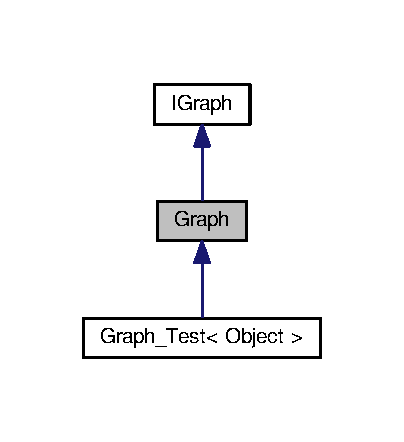
\includegraphics[width=194pt]{class_graph__inherit__graph}
\end{center}
\end{figure}


Diagram współpracy dla Graph\-:
\nopagebreak
\begin{figure}[H]
\begin{center}
\leavevmode
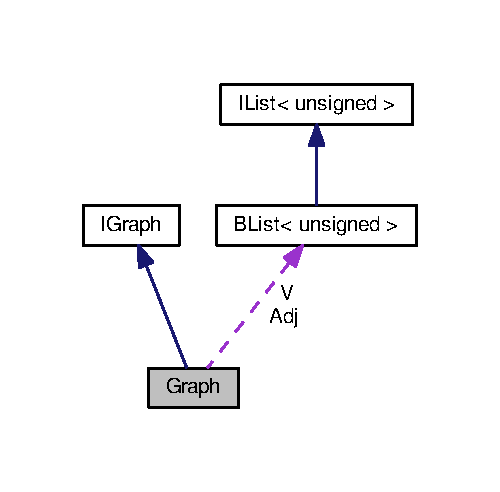
\includegraphics[width=240pt]{class_graph__coll__graph}
\end{center}
\end{figure}
\subsubsection*{Metody publiczne}
\begin{DoxyCompactItemize}
\item 
\hyperlink{class_graph_ae4c72b8ac4d693c49800a4c7e273654f}{Graph} ()
\begin{DoxyCompactList}\small\item\em Konstruktor grafu. \end{DoxyCompactList}\item 
\hyperlink{class_graph_a4112e28d02c5b96ff903e0c5ef23f754}{Graph} (int problem\-Size)
\begin{DoxyCompactList}\small\item\em Konstruktor grafu. \end{DoxyCompactList}\item 
\hyperlink{class_graph_a902c5b3eacb66d60752525ab23297a95}{$\sim$\-Graph} ()
\begin{DoxyCompactList}\small\item\em Destruktor grafu. \end{DoxyCompactList}\item 
\hyperlink{class_b_list}{B\-List}$<$ unsigned $>$ $\ast$ \hyperlink{class_graph_a7ba4e8932750650f1aa0ffac47ef6d53}{neighbours} (unsigned i)
\begin{DoxyCompactList}\small\item\em Podaje listę sąsiedztwa danego wierzchołka. \end{DoxyCompactList}\item 
virtual bool \hyperlink{class_graph_a6e15151dd48dbc8d88e9c69b9da1ce42}{are\-Adjacent} (unsigned i, unsigned j)
\begin{DoxyCompactList}\small\item\em Sprawdza, czy wierzchołki są sąsiadujące Szuka wierzchołka j na liście sąsiedztwa wierzchołka i. \end{DoxyCompactList}\item 
virtual void \hyperlink{class_graph_a2fbe0e22365c6ca537ad58cc41f762d3}{insert\-Vertex} (unsigned i)
\begin{DoxyCompactList}\small\item\em Dodaje wierzchołek Dodaje do listy wierzchołków. \end{DoxyCompactList}\item 
virtual void \hyperlink{class_graph_adcd035a684543785d45f5e595e642d04}{insert\-Edge} (unsigned i, unsigned j, unsigned w=1)
\begin{DoxyCompactList}\small\item\em Dodaje krawędź Dodaje wpisy na listach sąsiedztwa dla obu wierzchołków. \end{DoxyCompactList}\item 
\hyperlink{class_b_list}{B\-List}$<$ unsigned $>$ \& \hyperlink{class_graph_afa24fcfb647f26c4685749cb2415f65d}{vertices} ()
\begin{DoxyCompactList}\small\item\em Zwraca listę wierzchołków. \end{DoxyCompactList}\item 
int \& \hyperlink{class_graph_a8964ae826a9323ec3fd565dd3a90be24}{max\-N} ()
\begin{DoxyCompactList}\small\item\em Podaje maksymalną liczbę wierzchołków. \end{DoxyCompactList}\item 
void \hyperlink{class_graph_a8401c9a52f79166e118653cb40416764}{Print} ()
\begin{DoxyCompactList}\small\item\em Drukuje krawędzie grafu. \end{DoxyCompactList}\item 
void \hyperlink{class_graph_a8cc0bbeb0a745a071bf9f8caa4822889}{B\-F\-S} (unsigned i)
\begin{DoxyCompactList}\small\item\em Przechodzi graf wszerz Wykorzystuje implementację kolejki. \end{DoxyCompactList}\item 
void \hyperlink{class_graph_a799822f4b278f1ef2024a4d26a3c1c93}{D\-F\-S} (unsigned i)
\begin{DoxyCompactList}\small\item\em Przechodzi graf wgłąb Wykorzystuje implementację stosu. \end{DoxyCompactList}\end{DoxyCompactItemize}
\subsubsection*{Atrybuty chronione}
\begin{DoxyCompactItemize}
\item 
\hyperlink{class_b_list}{B\-List}$<$ unsigned $>$ \hyperlink{class_graph_ab2e9947e838cf65a60dfa3ec57367c45}{V}
\item 
\hyperlink{class_b_list}{B\-List}$<$ unsigned $>$ $\ast$ \hyperlink{class_graph_a666d457e13e81f8101235eb28f7f9d5a}{Adj}
\item 
int \hyperlink{class_graph_ae9cf5ba4841d02a2746033b68bd38764}{N}
\end{DoxyCompactItemize}


\subsubsection{Opis szczegółowy}


Definicja w linii 15 pliku Graph.\-hh.



\subsubsection{Dokumentacja konstruktora i destruktora}
\hypertarget{class_graph_ae4c72b8ac4d693c49800a4c7e273654f}{\index{Graph@{Graph}!Graph@{Graph}}
\index{Graph@{Graph}!Graph@{Graph}}
\paragraph[{Graph}]{\setlength{\rightskip}{0pt plus 5cm}Graph\-::\-Graph (
\begin{DoxyParamCaption}
{}
\end{DoxyParamCaption}
)}}\label{class_graph_ae4c72b8ac4d693c49800a4c7e273654f}


Konstruktor grafu. 

Inicjuje graf poprzez utworzenie tablicy list sąsiedztwa. Domyślnie 10 wierzchołków. 

Definicja w linii 118 pliku Graph.\-hh.

\hypertarget{class_graph_a4112e28d02c5b96ff903e0c5ef23f754}{\index{Graph@{Graph}!Graph@{Graph}}
\index{Graph@{Graph}!Graph@{Graph}}
\paragraph[{Graph}]{\setlength{\rightskip}{0pt plus 5cm}Graph\-::\-Graph (
\begin{DoxyParamCaption}
\item[{int}]{problem\-Size}
\end{DoxyParamCaption}
)}}\label{class_graph_a4112e28d02c5b96ff903e0c5ef23f754}


Konstruktor grafu. 

Inicjuje graf poprzez utworzenie tablicy list sąsiedztwa dla podanej liczby wierzchołków. 
\begin{DoxyParams}[1]{Parametry}
\mbox{\tt in}  & {\em problem\-Size} & -\/ liczba wierzchołków \\
\hline
\end{DoxyParams}


Definicja w linii 124 pliku Graph.\-hh.

\hypertarget{class_graph_a902c5b3eacb66d60752525ab23297a95}{\index{Graph@{Graph}!$\sim$\-Graph@{$\sim$\-Graph}}
\index{$\sim$\-Graph@{$\sim$\-Graph}!Graph@{Graph}}
\paragraph[{$\sim$\-Graph}]{\setlength{\rightskip}{0pt plus 5cm}Graph\-::$\sim$\-Graph (
\begin{DoxyParamCaption}
{}
\end{DoxyParamCaption}
)}}\label{class_graph_a902c5b3eacb66d60752525ab23297a95}


Destruktor grafu. 

Zwalnia pamięć zajmowaną przez tablicę list sąsiedztwa. Wywołuje destruktor listy wierzchołków. 

Definicja w linii 130 pliku Graph.\-hh.



\subsubsection{Dokumentacja funkcji składowych}
\hypertarget{class_graph_a6e15151dd48dbc8d88e9c69b9da1ce42}{\index{Graph@{Graph}!are\-Adjacent@{are\-Adjacent}}
\index{are\-Adjacent@{are\-Adjacent}!Graph@{Graph}}
\paragraph[{are\-Adjacent}]{\setlength{\rightskip}{0pt plus 5cm}bool Graph\-::are\-Adjacent (
\begin{DoxyParamCaption}
\item[{unsigned}]{i, }
\item[{unsigned}]{j}
\end{DoxyParamCaption}
)\hspace{0.3cm}{\ttfamily [virtual]}}}\label{class_graph_a6e15151dd48dbc8d88e9c69b9da1ce42}


Sprawdza, czy wierzchołki są sąsiadujące Szuka wierzchołka j na liście sąsiedztwa wierzchołka i. 


\begin{DoxyParams}[1]{Parametry}
\mbox{\tt in}  & {\em i} & -\/ wierzchołek pierwszy \\
\hline
\mbox{\tt in}  & {\em j} & -\/ wierzchołek druga \\
\hline
\end{DoxyParams}

\begin{DoxyRetVals}{Zwracane wartości}
{\em true} & -\/ jeśli są sąsiednie \\
\hline
{\em false} & -\/ jeśli nie są sąsiednie \\
\hline
\end{DoxyRetVals}


Implementuje \hyperlink{class_i_graph_a8562d602c3d98fa3bd483ca033806833}{I\-Graph}.



Definicja w linii 147 pliku Graph.\-hh.

\hypertarget{class_graph_a8cc0bbeb0a745a071bf9f8caa4822889}{\index{Graph@{Graph}!B\-F\-S@{B\-F\-S}}
\index{B\-F\-S@{B\-F\-S}!Graph@{Graph}}
\paragraph[{B\-F\-S}]{\setlength{\rightskip}{0pt plus 5cm}void Graph\-::\-B\-F\-S (
\begin{DoxyParamCaption}
\item[{unsigned}]{i}
\end{DoxyParamCaption}
)}}\label{class_graph_a8cc0bbeb0a745a071bf9f8caa4822889}


Przechodzi graf wszerz Wykorzystuje implementację kolejki. 


\begin{DoxyParams}[1]{Parametry}
\mbox{\tt in}  & {\em i} & -\/ numer wierzchołka startowego \\
\hline
\end{DoxyParams}


Definicja w linii 185 pliku Graph.\-hh.

\hypertarget{class_graph_a799822f4b278f1ef2024a4d26a3c1c93}{\index{Graph@{Graph}!D\-F\-S@{D\-F\-S}}
\index{D\-F\-S@{D\-F\-S}!Graph@{Graph}}
\paragraph[{D\-F\-S}]{\setlength{\rightskip}{0pt plus 5cm}void Graph\-::\-D\-F\-S (
\begin{DoxyParamCaption}
\item[{unsigned}]{i}
\end{DoxyParamCaption}
)}}\label{class_graph_a799822f4b278f1ef2024a4d26a3c1c93}


Przechodzi graf wgłąb Wykorzystuje implementację stosu. 


\begin{DoxyParams}[1]{Parametry}
\mbox{\tt in}  & {\em i} & -\/ numer wierzchołka startowego \\
\hline
\end{DoxyParams}


Definicja w linii 219 pliku Graph.\-hh.

\hypertarget{class_graph_adcd035a684543785d45f5e595e642d04}{\index{Graph@{Graph}!insert\-Edge@{insert\-Edge}}
\index{insert\-Edge@{insert\-Edge}!Graph@{Graph}}
\paragraph[{insert\-Edge}]{\setlength{\rightskip}{0pt plus 5cm}void Graph\-::insert\-Edge (
\begin{DoxyParamCaption}
\item[{unsigned}]{i, }
\item[{unsigned}]{j, }
\item[{unsigned}]{w = {\ttfamily 1}}
\end{DoxyParamCaption}
)\hspace{0.3cm}{\ttfamily [virtual]}}}\label{class_graph_adcd035a684543785d45f5e595e642d04}


Dodaje krawędź Dodaje wpisy na listach sąsiedztwa dla obu wierzchołków. 


\begin{DoxyParams}[1]{Parametry}
\mbox{\tt in}  & {\em i} & -\/ numer wierzchołka pierwszego \\
\hline
\mbox{\tt in}  & {\em j} & -\/ numer wierzchołka drugiego \\
\hline
\mbox{\tt in}  & {\em w} & -\/ waga krawędzi \\
\hline
\end{DoxyParams}


Implementuje \hyperlink{class_i_graph_a95fca9dcbc82ef1c20d15b51d015b847}{I\-Graph}.



Definicja w linii 162 pliku Graph.\-hh.

\hypertarget{class_graph_a2fbe0e22365c6ca537ad58cc41f762d3}{\index{Graph@{Graph}!insert\-Vertex@{insert\-Vertex}}
\index{insert\-Vertex@{insert\-Vertex}!Graph@{Graph}}
\paragraph[{insert\-Vertex}]{\setlength{\rightskip}{0pt plus 5cm}void Graph\-::insert\-Vertex (
\begin{DoxyParamCaption}
\item[{unsigned}]{i}
\end{DoxyParamCaption}
)\hspace{0.3cm}{\ttfamily [virtual]}}}\label{class_graph_a2fbe0e22365c6ca537ad58cc41f762d3}


Dodaje wierzchołek Dodaje do listy wierzchołków. 


\begin{DoxyParams}[1]{Parametry}
\mbox{\tt in}  & {\em i} & -\/ numer wierzchołka \\
\hline
\end{DoxyParams}


Implementuje \hyperlink{class_i_graph_a78668f8067a9a0d108bfc4ef719ba206}{I\-Graph}.



Definicja w linii 156 pliku Graph.\-hh.

\hypertarget{class_graph_a8964ae826a9323ec3fd565dd3a90be24}{\index{Graph@{Graph}!max\-N@{max\-N}}
\index{max\-N@{max\-N}!Graph@{Graph}}
\paragraph[{max\-N}]{\setlength{\rightskip}{0pt plus 5cm}int\& Graph\-::max\-N (
\begin{DoxyParamCaption}
{}
\end{DoxyParamCaption}
)\hspace{0.3cm}{\ttfamily [inline]}}}\label{class_graph_a8964ae826a9323ec3fd565dd3a90be24}


Podaje maksymalną liczbę wierzchołków. 

\begin{DoxyReturn}{Zwraca}
rozmiar tablicy list sąsiedztwa 
\end{DoxyReturn}


Definicja w linii 96 pliku Graph.\-hh.

\hypertarget{class_graph_a7ba4e8932750650f1aa0ffac47ef6d53}{\index{Graph@{Graph}!neighbours@{neighbours}}
\index{neighbours@{neighbours}!Graph@{Graph}}
\paragraph[{neighbours}]{\setlength{\rightskip}{0pt plus 5cm}{\bf B\-List}$<$ unsigned $>$ $\ast$ Graph\-::neighbours (
\begin{DoxyParamCaption}
\item[{unsigned}]{i}
\end{DoxyParamCaption}
)}}\label{class_graph_a7ba4e8932750650f1aa0ffac47ef6d53}


Podaje listę sąsiedztwa danego wierzchołka. 


\begin{DoxyParams}[1]{Parametry}
\mbox{\tt in}  & {\em i} & -\/ wierzchołek, którego lista sąsiedztwa ma być zwrócona \\
\hline
\end{DoxyParams}
\begin{DoxyReturn}{Zwraca}
wskaźnik na lista sąsiedztwa podanego wierzchołka 
\end{DoxyReturn}


Definicja w linii 139 pliku Graph.\-hh.

\hypertarget{class_graph_a8401c9a52f79166e118653cb40416764}{\index{Graph@{Graph}!Print@{Print}}
\index{Print@{Print}!Graph@{Graph}}
\paragraph[{Print}]{\setlength{\rightskip}{0pt plus 5cm}void Graph\-::\-Print (
\begin{DoxyParamCaption}
{}
\end{DoxyParamCaption}
)}}\label{class_graph_a8401c9a52f79166e118653cb40416764}


Drukuje krawędzie grafu. 



Definicja w linii 175 pliku Graph.\-hh.

\hypertarget{class_graph_afa24fcfb647f26c4685749cb2415f65d}{\index{Graph@{Graph}!vertices@{vertices}}
\index{vertices@{vertices}!Graph@{Graph}}
\paragraph[{vertices}]{\setlength{\rightskip}{0pt plus 5cm}{\bf B\-List}$<$unsigned$>$\& Graph\-::vertices (
\begin{DoxyParamCaption}
{}
\end{DoxyParamCaption}
)\hspace{0.3cm}{\ttfamily [inline]}}}\label{class_graph_afa24fcfb647f26c4685749cb2415f65d}


Zwraca listę wierzchołków. 

\begin{DoxyReturn}{Zwraca}
lista sąsiedztwa podanego wierzchołka 
\end{DoxyReturn}


Definicja w linii 90 pliku Graph.\-hh.



\subsubsection{Dokumentacja atrybutów składowych}
\hypertarget{class_graph_a666d457e13e81f8101235eb28f7f9d5a}{\index{Graph@{Graph}!Adj@{Adj}}
\index{Adj@{Adj}!Graph@{Graph}}
\paragraph[{Adj}]{\setlength{\rightskip}{0pt plus 5cm}{\bf B\-List}$<$unsigned$>$$\ast$ Graph\-::\-Adj\hspace{0.3cm}{\ttfamily [protected]}}}\label{class_graph_a666d457e13e81f8101235eb28f7f9d5a}
-\/$>$ lista wierzchołków 

Definicja w linii 19 pliku Graph.\-hh.

\hypertarget{class_graph_ae9cf5ba4841d02a2746033b68bd38764}{\index{Graph@{Graph}!N@{N}}
\index{N@{N}!Graph@{Graph}}
\paragraph[{N}]{\setlength{\rightskip}{0pt plus 5cm}int Graph\-::\-N\hspace{0.3cm}{\ttfamily [protected]}}}\label{class_graph_ae9cf5ba4841d02a2746033b68bd38764}
-\/$>$ tablica list sąsiedztwa 

Definicja w linii 20 pliku Graph.\-hh.

\hypertarget{class_graph_ab2e9947e838cf65a60dfa3ec57367c45}{\index{Graph@{Graph}!V@{V}}
\index{V@{V}!Graph@{Graph}}
\paragraph[{V}]{\setlength{\rightskip}{0pt plus 5cm}{\bf B\-List}$<$unsigned$>$ Graph\-::\-V\hspace{0.3cm}{\ttfamily [protected]}}}\label{class_graph_ab2e9947e838cf65a60dfa3ec57367c45}


Definicja w linii 18 pliku Graph.\-hh.



Dokumentacja dla tej klasy została wygenerowana z pliku\-:\begin{DoxyCompactItemize}
\item 
prj/inc/\hyperlink{_graph_8hh}{Graph.\-hh}\end{DoxyCompactItemize}

\hypertarget{class_graph___test}{\subsection{Dokumentacja szablonu klasy Graph\-\_\-\-Test$<$ Object $>$}
\label{class_graph___test}\index{Graph\-\_\-\-Test$<$ Object $>$@{Graph\-\_\-\-Test$<$ Object $>$}}
}


Szablonowa klasa implementująca testowy graf.  




{\ttfamily \#include $<$Graph\-\_\-\-Test.\-hh$>$}



Diagram dziedziczenia dla Graph\-\_\-\-Test$<$ Object $>$
\nopagebreak
\begin{figure}[H]
\begin{center}
\leavevmode
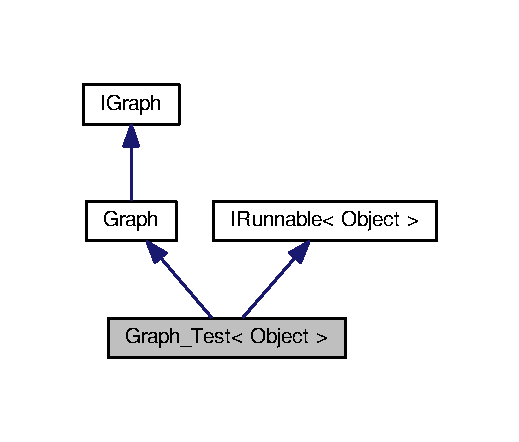
\includegraphics[width=249pt]{class_graph___test__inherit__graph}
\end{center}
\end{figure}


Diagram współpracy dla Graph\-\_\-\-Test$<$ Object $>$\-:
\nopagebreak
\begin{figure}[H]
\begin{center}
\leavevmode
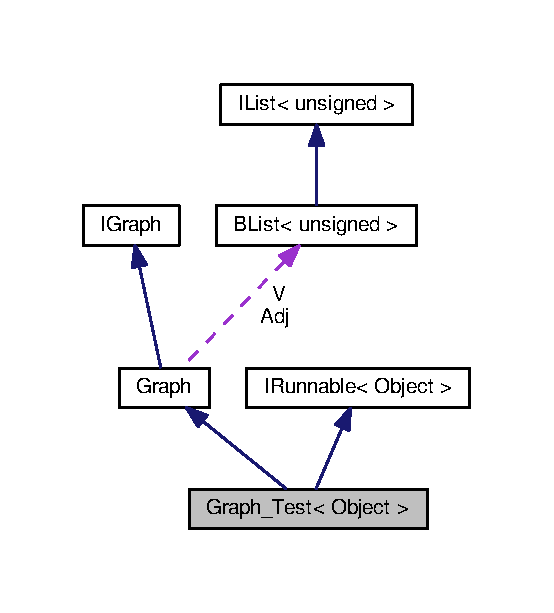
\includegraphics[width=266pt]{class_graph___test__coll__graph}
\end{center}
\end{figure}
\subsubsection*{Metody publiczne}
\begin{DoxyCompactItemize}
\item 
void \hyperlink{class_graph___test_aa82baee1265ff1172c802b1fdfdf1290}{change\-Search\-Type} (char type)
\begin{DoxyCompactList}\small\item\em Zmienia sposób przechodzenia grafu. \end{DoxyCompactList}\item 
virtual bool \hyperlink{class_graph___test_acbad8d61bca15e38751e9877c3bfe70d}{Prepare} (Object parametr)
\begin{DoxyCompactList}\small\item\em Metoda przygotowująca graf W zależności od podanej liczby, dodaje odpowiednio dużo wierzchołków do grafu i tworzy między nimi spójne powiązanie. W następujący sposób\-: tworzy tymczasową tablicę z numerami wierzchołków i następnie losowo zamienia komórki tablicy. Następnie dodaje krawędzie zgodnie z wylosowaną kolejnością. Na koniec generuje 2n losowych krawędzi. \end{DoxyCompactList}\item 
virtual bool \hyperlink{class_graph___test_a1f7ecb202fa8d6f02fc2639b9af2ee4a}{Run} ()
\begin{DoxyCompactList}\small\item\em Metoda uruchamiająca przejście grafu W zależności od ustawienia parametru search\-Type, uruchamia przejście B\-F\-S lub D\-F\-S. \end{DoxyCompactList}\end{DoxyCompactItemize}
\subsubsection*{Dodatkowe Dziedziczone Składowe}


\subsubsection{Opis szczegółowy}
\subsubsection*{template$<$typename Object$>$class Graph\-\_\-\-Test$<$ Object $>$}

Szablonowa klasa implementująca testowy graf. 

Definicja w linii 17 pliku Graph\-\_\-\-Test.\-hh.



\subsubsection{Dokumentacja funkcji składowych}
\hypertarget{class_graph___test_aa82baee1265ff1172c802b1fdfdf1290}{\index{Graph\-\_\-\-Test@{Graph\-\_\-\-Test}!change\-Search\-Type@{change\-Search\-Type}}
\index{change\-Search\-Type@{change\-Search\-Type}!Graph_Test@{Graph\-\_\-\-Test}}
\paragraph[{change\-Search\-Type}]{\setlength{\rightskip}{0pt plus 5cm}template$<$typename Object $>$ void {\bf Graph\-\_\-\-Test}$<$ Object $>$\-::change\-Search\-Type (
\begin{DoxyParamCaption}
\item[{char}]{type}
\end{DoxyParamCaption}
)}}\label{class_graph___test_aa82baee1265ff1172c802b1fdfdf1290}


Zmienia sposób przechodzenia grafu. 

Ustawia podany typ znakowy jako wyznacznik przejścia grafu metodą B\-F\-S lub D\-F\-S. 

Definicja w linii 56 pliku Graph\-\_\-\-Test.\-hh.

\hypertarget{class_graph___test_acbad8d61bca15e38751e9877c3bfe70d}{\index{Graph\-\_\-\-Test@{Graph\-\_\-\-Test}!Prepare@{Prepare}}
\index{Prepare@{Prepare}!Graph_Test@{Graph\-\_\-\-Test}}
\paragraph[{Prepare}]{\setlength{\rightskip}{0pt plus 5cm}template$<$typename Object $>$ bool {\bf Graph\-\_\-\-Test}$<$ Object $>$\-::Prepare (
\begin{DoxyParamCaption}
\item[{Object}]{parametr}
\end{DoxyParamCaption}
)\hspace{0.3cm}{\ttfamily [virtual]}}}\label{class_graph___test_acbad8d61bca15e38751e9877c3bfe70d}


Metoda przygotowująca graf W zależności od podanej liczby, dodaje odpowiednio dużo wierzchołków do grafu i tworzy między nimi spójne powiązanie. W następujący sposób\-: tworzy tymczasową tablicę z numerami wierzchołków i następnie losowo zamienia komórki tablicy. Następnie dodaje krawędzie zgodnie z wylosowaną kolejnością. Na koniec generuje 2n losowych krawędzi. 


\begin{DoxyParams}[1]{Parametry}
\mbox{\tt in}  & {\em parametr} & -\/ liczba wierzchołków \\
\hline
\end{DoxyParams}

\begin{DoxyRetVals}{Zwracane wartości}
{\em true} & -\/ jeśli operacja zakończyła się pomyślnie \\
\hline
{\em false} & -\/ jeśli wystąpił jakiś błąd \\
\hline
\end{DoxyRetVals}


Implementuje \hyperlink{class_i_runnable_a25fb85d8692bfedad61b81f875c6e358}{I\-Runnable$<$ Object $>$}.



Definicja w linii 62 pliku Graph\-\_\-\-Test.\-hh.

\hypertarget{class_graph___test_a1f7ecb202fa8d6f02fc2639b9af2ee4a}{\index{Graph\-\_\-\-Test@{Graph\-\_\-\-Test}!Run@{Run}}
\index{Run@{Run}!Graph_Test@{Graph\-\_\-\-Test}}
\paragraph[{Run}]{\setlength{\rightskip}{0pt plus 5cm}template$<$typename Object $>$ bool {\bf Graph\-\_\-\-Test}$<$ Object $>$\-::Run (
\begin{DoxyParamCaption}
{}
\end{DoxyParamCaption}
)\hspace{0.3cm}{\ttfamily [virtual]}}}\label{class_graph___test_a1f7ecb202fa8d6f02fc2639b9af2ee4a}


Metoda uruchamiająca przejście grafu W zależności od ustawienia parametru search\-Type, uruchamia przejście B\-F\-S lub D\-F\-S. 


\begin{DoxyRetVals}{Zwracane wartości}
{\em true} & -\/ jeśli operacja zakończyła się pomyślnie \\
\hline
{\em false} & -\/ jeśli wystąpił jakiś błąd \\
\hline
\end{DoxyRetVals}


Implementuje \hyperlink{class_i_runnable_aff6851ded59d477d30c2ef01664b25fe}{I\-Runnable$<$ Object $>$}.



Definicja w linii 101 pliku Graph\-\_\-\-Test.\-hh.



Dokumentacja dla tej klasy została wygenerowana z pliku\-:\begin{DoxyCompactItemize}
\item 
prj/inc/\hyperlink{_graph___test_8hh}{Graph\-\_\-\-Test.\-hh}\end{DoxyCompactItemize}

\hypertarget{class_i_graph}{\subsection{Dokumentacja klasy I\-Graph}
\label{class_i_graph}\index{I\-Graph@{I\-Graph}}
}


{\ttfamily \#include $<$I\-Graph.\-hh$>$}



Diagram dziedziczenia dla I\-Graph
\nopagebreak
\begin{figure}[H]
\begin{center}
\leavevmode
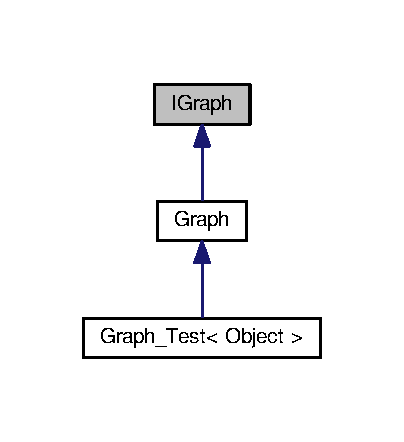
\includegraphics[width=194pt]{class_i_graph__inherit__graph}
\end{center}
\end{figure}
\subsubsection*{Metody publiczne}
\begin{DoxyCompactItemize}
\item 
virtual bool \hyperlink{class_i_graph_a8562d602c3d98fa3bd483ca033806833}{are\-Adjacent} (unsigned i, unsigned j)=0
\item 
virtual void \hyperlink{class_i_graph_a78668f8067a9a0d108bfc4ef719ba206}{insert\-Vertex} (unsigned i)=0
\item 
virtual void \hyperlink{class_i_graph_a95fca9dcbc82ef1c20d15b51d015b847}{insert\-Edge} (unsigned i, unsigned j, unsigned w=1)=0
\end{DoxyCompactItemize}


\subsubsection{Opis szczegółowy}


Definicja w linii 13 pliku I\-Graph.\-hh.



\subsubsection{Dokumentacja funkcji składowych}
\hypertarget{class_i_graph_a8562d602c3d98fa3bd483ca033806833}{\index{I\-Graph@{I\-Graph}!are\-Adjacent@{are\-Adjacent}}
\index{are\-Adjacent@{are\-Adjacent}!IGraph@{I\-Graph}}
\paragraph[{are\-Adjacent}]{\setlength{\rightskip}{0pt plus 5cm}virtual bool I\-Graph\-::are\-Adjacent (
\begin{DoxyParamCaption}
\item[{unsigned}]{i, }
\item[{unsigned}]{j}
\end{DoxyParamCaption}
)\hspace{0.3cm}{\ttfamily [pure virtual]}}}\label{class_i_graph_a8562d602c3d98fa3bd483ca033806833}


Implementowany w \hyperlink{class_graph_a6e15151dd48dbc8d88e9c69b9da1ce42}{Graph}.

\hypertarget{class_i_graph_a95fca9dcbc82ef1c20d15b51d015b847}{\index{I\-Graph@{I\-Graph}!insert\-Edge@{insert\-Edge}}
\index{insert\-Edge@{insert\-Edge}!IGraph@{I\-Graph}}
\paragraph[{insert\-Edge}]{\setlength{\rightskip}{0pt plus 5cm}virtual void I\-Graph\-::insert\-Edge (
\begin{DoxyParamCaption}
\item[{unsigned}]{i, }
\item[{unsigned}]{j, }
\item[{unsigned}]{w = {\ttfamily 1}}
\end{DoxyParamCaption}
)\hspace{0.3cm}{\ttfamily [pure virtual]}}}\label{class_i_graph_a95fca9dcbc82ef1c20d15b51d015b847}


Implementowany w \hyperlink{class_graph_adcd035a684543785d45f5e595e642d04}{Graph}.

\hypertarget{class_i_graph_a78668f8067a9a0d108bfc4ef719ba206}{\index{I\-Graph@{I\-Graph}!insert\-Vertex@{insert\-Vertex}}
\index{insert\-Vertex@{insert\-Vertex}!IGraph@{I\-Graph}}
\paragraph[{insert\-Vertex}]{\setlength{\rightskip}{0pt plus 5cm}virtual void I\-Graph\-::insert\-Vertex (
\begin{DoxyParamCaption}
\item[{unsigned}]{i}
\end{DoxyParamCaption}
)\hspace{0.3cm}{\ttfamily [pure virtual]}}}\label{class_i_graph_a78668f8067a9a0d108bfc4ef719ba206}


Implementowany w \hyperlink{class_graph_a2fbe0e22365c6ca537ad58cc41f762d3}{Graph}.



Dokumentacja dla tej klasy została wygenerowana z pliku\-:\begin{DoxyCompactItemize}
\item 
prj/inc/\hyperlink{_i_graph_8hh}{I\-Graph.\-hh}\end{DoxyCompactItemize}

\hypertarget{class_i_list}{\subsection{Dokumentacja szablonu klasy I\-List$<$ Object $>$}
\label{class_i_list}\index{I\-List$<$ Object $>$@{I\-List$<$ Object $>$}}
}


Interfejs listy dwukierunkowej.  




{\ttfamily \#include $<$I\-List.\-hh$>$}



Diagram dziedziczenia dla I\-List$<$ Object $>$
\nopagebreak
\begin{figure}[H]
\begin{center}
\leavevmode
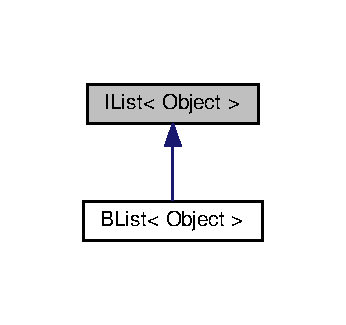
\includegraphics[width=166pt]{class_i_list__inherit__graph}
\end{center}
\end{figure}
\subsubsection*{Metody publiczne}
\begin{DoxyCompactItemize}
\item 
virtual bool \hyperlink{class_i_list_a6a67d956d023bd003fd4a19e766d475c}{Is\-Empty} ()=0
\begin{DoxyCompactList}\small\item\em Metoda sprawdzająca, czy lista jest pusta. \end{DoxyCompactList}\item 
virtual void \hyperlink{class_i_list_a8015c8bd4e35161d31f863e74e943329}{Add\-Front} (const Object new\-Item)=0
\item 
virtual void \hyperlink{class_i_list_a62af6638df7793dc5696c716122e1fc8}{Add\-Back} (const Object new\-Item)=0
\item 
virtual const Object \& \hyperlink{class_i_list_a61e3afad71d99da6b85148e61fa01e9b}{Remove\-Front} ()=0
\item 
virtual const Object \& \hyperlink{class_i_list_ab4db42b40d2b583a26b1c3b398769e15}{Remove\-Back} ()=0
\end{DoxyCompactItemize}


\subsubsection{Opis szczegółowy}
\subsubsection*{template$<$typename Object$>$class I\-List$<$ Object $>$}

Interfejs listy dwukierunkowej. 

Definiuje A\-D\-T dla listy dwukierunkowej.

Lista może przechowywać dowolny typ danych dzięki zastosowaniu szablonu. 

Definicja w linii 22 pliku I\-List.\-hh.



\subsubsection{Dokumentacja funkcji składowych}
\hypertarget{class_i_list_a62af6638df7793dc5696c716122e1fc8}{\index{I\-List@{I\-List}!Add\-Back@{Add\-Back}}
\index{Add\-Back@{Add\-Back}!IList@{I\-List}}
\paragraph[{Add\-Back}]{\setlength{\rightskip}{0pt plus 5cm}template$<$typename Object$>$ virtual void {\bf I\-List}$<$ Object $>$\-::Add\-Back (
\begin{DoxyParamCaption}
\item[{const Object}]{new\-Item}
\end{DoxyParamCaption}
)\hspace{0.3cm}{\ttfamily [pure virtual]}}}\label{class_i_list_a62af6638df7793dc5696c716122e1fc8}


Implementowany w \hyperlink{class_b_list_aacb4abd5a4dbe72dbf448d299eb4c6b8}{B\-List$<$ Object $>$} i \hyperlink{class_b_list_aacb4abd5a4dbe72dbf448d299eb4c6b8}{B\-List$<$ unsigned $>$}.

\hypertarget{class_i_list_a8015c8bd4e35161d31f863e74e943329}{\index{I\-List@{I\-List}!Add\-Front@{Add\-Front}}
\index{Add\-Front@{Add\-Front}!IList@{I\-List}}
\paragraph[{Add\-Front}]{\setlength{\rightskip}{0pt plus 5cm}template$<$typename Object$>$ virtual void {\bf I\-List}$<$ Object $>$\-::Add\-Front (
\begin{DoxyParamCaption}
\item[{const Object}]{new\-Item}
\end{DoxyParamCaption}
)\hspace{0.3cm}{\ttfamily [pure virtual]}}}\label{class_i_list_a8015c8bd4e35161d31f863e74e943329}


Implementowany w \hyperlink{class_b_list_a3ce77cc9d73682bfac57c70dafdce89d}{B\-List$<$ Object $>$} i \hyperlink{class_b_list_a3ce77cc9d73682bfac57c70dafdce89d}{B\-List$<$ unsigned $>$}.

\hypertarget{class_i_list_a6a67d956d023bd003fd4a19e766d475c}{\index{I\-List@{I\-List}!Is\-Empty@{Is\-Empty}}
\index{Is\-Empty@{Is\-Empty}!IList@{I\-List}}
\paragraph[{Is\-Empty}]{\setlength{\rightskip}{0pt plus 5cm}template$<$typename Object$>$ virtual bool {\bf I\-List}$<$ Object $>$\-::Is\-Empty (
\begin{DoxyParamCaption}
{}
\end{DoxyParamCaption}
)\hspace{0.3cm}{\ttfamily [pure virtual]}}}\label{class_i_list_a6a67d956d023bd003fd4a19e766d475c}


Metoda sprawdzająca, czy lista jest pusta. 

true -\/ jeśli lista jest pusta  truefalse -\/ jeśli nie jest pusta 

Implementowany w \hyperlink{class_b_list_ae69bf69a67a46e5a3a0a9ba743354b2b}{B\-List$<$ Object $>$} i \hyperlink{class_b_list_ae69bf69a67a46e5a3a0a9ba743354b2b}{B\-List$<$ unsigned $>$}.

\hypertarget{class_i_list_ab4db42b40d2b583a26b1c3b398769e15}{\index{I\-List@{I\-List}!Remove\-Back@{Remove\-Back}}
\index{Remove\-Back@{Remove\-Back}!IList@{I\-List}}
\paragraph[{Remove\-Back}]{\setlength{\rightskip}{0pt plus 5cm}template$<$typename Object$>$ virtual const Object\& {\bf I\-List}$<$ Object $>$\-::Remove\-Back (
\begin{DoxyParamCaption}
{}
\end{DoxyParamCaption}
)\hspace{0.3cm}{\ttfamily [pure virtual]}}}\label{class_i_list_ab4db42b40d2b583a26b1c3b398769e15}


Implementowany w \hyperlink{class_b_list_a4df7a72e29bfb324ca366fc2322184ea}{B\-List$<$ Object $>$} i \hyperlink{class_b_list_a4df7a72e29bfb324ca366fc2322184ea}{B\-List$<$ unsigned $>$}.

\hypertarget{class_i_list_a61e3afad71d99da6b85148e61fa01e9b}{\index{I\-List@{I\-List}!Remove\-Front@{Remove\-Front}}
\index{Remove\-Front@{Remove\-Front}!IList@{I\-List}}
\paragraph[{Remove\-Front}]{\setlength{\rightskip}{0pt plus 5cm}template$<$typename Object$>$ virtual const Object\& {\bf I\-List}$<$ Object $>$\-::Remove\-Front (
\begin{DoxyParamCaption}
{}
\end{DoxyParamCaption}
)\hspace{0.3cm}{\ttfamily [pure virtual]}}}\label{class_i_list_a61e3afad71d99da6b85148e61fa01e9b}


Implementowany w \hyperlink{class_b_list_a510b274bdcccf50699b41233a5f42a5f}{B\-List$<$ Object $>$} i \hyperlink{class_b_list_a510b274bdcccf50699b41233a5f42a5f}{B\-List$<$ unsigned $>$}.



Dokumentacja dla tej klasy została wygenerowana z pliku\-:\begin{DoxyCompactItemize}
\item 
prj/inc/\hyperlink{_i_list_8hh}{I\-List.\-hh}\end{DoxyCompactItemize}

\hypertarget{class_i_queue}{\subsection{Dokumentacja szablonu klasy I\-Queue$<$ Object $>$}
\label{class_i_queue}\index{I\-Queue$<$ Object $>$@{I\-Queue$<$ Object $>$}}
}


Klasa modelująca interfejs kolejki.  




{\ttfamily \#include $<$I\-Queue.\-hh$>$}



Diagram dziedziczenia dla I\-Queue$<$ Object $>$
\nopagebreak
\begin{figure}[H]
\begin{center}
\leavevmode
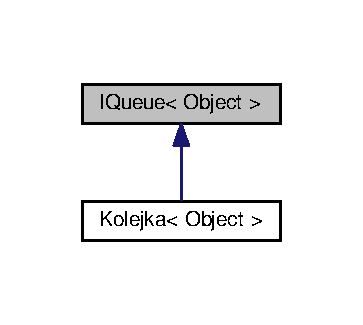
\includegraphics[width=174pt]{class_i_queue__inherit__graph}
\end{center}
\end{figure}
\subsubsection*{Metody publiczne}
\begin{DoxyCompactItemize}
\item 
virtual bool \hyperlink{class_i_queue_ae1c9e42be6ff647666c4468d3eec55a1}{Is\-Empty} ()=0
\begin{DoxyCompactList}\small\item\em Metoda sprawdzająca, czy lista jest pusta. \end{DoxyCompactList}\item 
virtual Object \hyperlink{class_i_queue_ab07e072ad92e4e93d57a0d3950c72764}{Front} ()=0
\begin{DoxyCompactList}\small\item\em Metoda zwracająca pierwszy element kolejki. \end{DoxyCompactList}\item 
virtual void \hyperlink{class_i_queue_af818d0fb70a5d088e6088c42f51df7e1}{Enqueue} (Object item)=0
\begin{DoxyCompactList}\small\item\em Metoda dodająca element do kolejki. \end{DoxyCompactList}\item 
virtual Object \hyperlink{class_i_queue_a6836f64bdf7102fdda590f21f7e5e208}{Dequeue} ()=0
\begin{DoxyCompactList}\small\item\em Metoda usuwająca element kolejki. \end{DoxyCompactList}\end{DoxyCompactItemize}


\subsubsection{Opis szczegółowy}
\subsubsection*{template$<$typename Object$>$class I\-Queue$<$ Object $>$}

Klasa modelująca interfejs kolejki. 

Definiuje A\-D\-T dla kolejki.

\hyperlink{class_kolejka}{Kolejka} może przechowywać dowolny typ danych dzięki zastosowaniu szablonu. 

Definicja w linii 22 pliku I\-Queue.\-hh.



\subsubsection{Dokumentacja funkcji składowych}
\hypertarget{class_i_queue_a6836f64bdf7102fdda590f21f7e5e208}{\index{I\-Queue@{I\-Queue}!Dequeue@{Dequeue}}
\index{Dequeue@{Dequeue}!IQueue@{I\-Queue}}
\paragraph[{Dequeue}]{\setlength{\rightskip}{0pt plus 5cm}template$<$typename Object $>$ virtual Object {\bf I\-Queue}$<$ Object $>$\-::Dequeue (
\begin{DoxyParamCaption}
{}
\end{DoxyParamCaption}
)\hspace{0.3cm}{\ttfamily [pure virtual]}}}\label{class_i_queue_a6836f64bdf7102fdda590f21f7e5e208}


Metoda usuwająca element kolejki. 

Usuwa element z początki kolejki. \begin{DoxyReturn}{Zwraca}
pierwszy element kolejki 
\end{DoxyReturn}


Implementowany w \hyperlink{class_kolejka_a61f6ec1436c1e95ce8675c8ccaf3e469}{Kolejka$<$ Object $>$}.

\hypertarget{class_i_queue_af818d0fb70a5d088e6088c42f51df7e1}{\index{I\-Queue@{I\-Queue}!Enqueue@{Enqueue}}
\index{Enqueue@{Enqueue}!IQueue@{I\-Queue}}
\paragraph[{Enqueue}]{\setlength{\rightskip}{0pt plus 5cm}template$<$typename Object $>$ virtual void {\bf I\-Queue}$<$ Object $>$\-::Enqueue (
\begin{DoxyParamCaption}
\item[{Object}]{item}
\end{DoxyParamCaption}
)\hspace{0.3cm}{\ttfamily [pure virtual]}}}\label{class_i_queue_af818d0fb70a5d088e6088c42f51df7e1}


Metoda dodająca element do kolejki. 

Ustawia element na koniec kolejki. 
\begin{DoxyParams}[1]{Parametry}
\mbox{\tt in}  & {\em item} & -\/ element do dodania \\
\hline
\end{DoxyParams}


Implementowany w \hyperlink{class_kolejka_a726ad18814137293bfdfd0500da27038}{Kolejka$<$ Object $>$}.

\hypertarget{class_i_queue_ab07e072ad92e4e93d57a0d3950c72764}{\index{I\-Queue@{I\-Queue}!Front@{Front}}
\index{Front@{Front}!IQueue@{I\-Queue}}
\paragraph[{Front}]{\setlength{\rightskip}{0pt plus 5cm}template$<$typename Object $>$ virtual Object {\bf I\-Queue}$<$ Object $>$\-::Front (
\begin{DoxyParamCaption}
{}
\end{DoxyParamCaption}
)\hspace{0.3cm}{\ttfamily [pure virtual]}}}\label{class_i_queue_ab07e072ad92e4e93d57a0d3950c72764}


Metoda zwracająca pierwszy element kolejki. 

\begin{DoxyReturn}{Zwraca}
pierwszy element kolejki 
\end{DoxyReturn}


Implementowany w \hyperlink{class_kolejka_a04e41ef06540e8a5f5338da175f26a1f}{Kolejka$<$ Object $>$}.

\hypertarget{class_i_queue_ae1c9e42be6ff647666c4468d3eec55a1}{\index{I\-Queue@{I\-Queue}!Is\-Empty@{Is\-Empty}}
\index{Is\-Empty@{Is\-Empty}!IQueue@{I\-Queue}}
\paragraph[{Is\-Empty}]{\setlength{\rightskip}{0pt plus 5cm}template$<$typename Object $>$ virtual bool {\bf I\-Queue}$<$ Object $>$\-::Is\-Empty (
\begin{DoxyParamCaption}
{}
\end{DoxyParamCaption}
)\hspace{0.3cm}{\ttfamily [pure virtual]}}}\label{class_i_queue_ae1c9e42be6ff647666c4468d3eec55a1}


Metoda sprawdzająca, czy lista jest pusta. 

true -\/ jeśli lista jest pusta  false -\/ jeśli nie jest pusta 

Implementowany w \hyperlink{class_kolejka_a15a8e2eff269ee2d6264af30cfd23cb2}{Kolejka$<$ Object $>$}.



Dokumentacja dla tej klasy została wygenerowana z pliku\-:\begin{DoxyCompactItemize}
\item 
prj/inc/\hyperlink{_i_queue_8hh}{I\-Queue.\-hh}\end{DoxyCompactItemize}

\hypertarget{class_i_runnable}{\subsection{Dokumentacja szablonu klasy I\-Runnable$<$ Object $>$}
\label{class_i_runnable}\index{I\-Runnable$<$ Object $>$@{I\-Runnable$<$ Object $>$}}
}


Klasa szablonowa modelująca interfejs \char`\"{}\-Biegacza\char`\"{}.  




{\ttfamily \#include $<$I\-Runnable.\-hh$>$}



Diagram dziedziczenia dla I\-Runnable$<$ Object $>$
\nopagebreak
\begin{figure}[H]
\begin{center}
\leavevmode
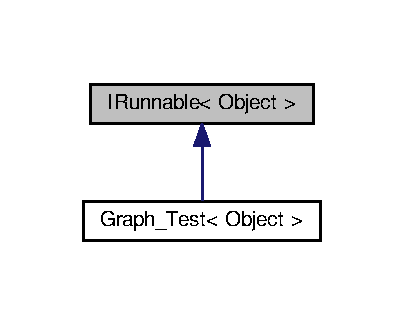
\includegraphics[width=194pt]{class_i_runnable__inherit__graph}
\end{center}
\end{figure}
\subsubsection*{Metody publiczne}
\begin{DoxyCompactItemize}
\item 
virtual bool \hyperlink{class_i_runnable_a25fb85d8692bfedad61b81f875c6e358}{Prepare} (Object parametr)=0
\begin{DoxyCompactList}\small\item\em Metoda przygotowująca obiekt do operacji. \end{DoxyCompactList}\item 
virtual bool \hyperlink{class_i_runnable_aff6851ded59d477d30c2ef01664b25fe}{Run} ()=0
\begin{DoxyCompactList}\small\item\em Metoda uruchamiająca zdefiniowaną operację \end{DoxyCompactList}\end{DoxyCompactItemize}


\subsubsection{Opis szczegółowy}
\subsubsection*{template$<$typename Object$>$class I\-Runnable$<$ Object $>$}

Klasa szablonowa modelująca interfejs \char`\"{}\-Biegacza\char`\"{}. 

Klasa jest abstrakcyjnym uogólnieniem obiektu, na którym można wykonać zdefiniowane operacje, którym z kolei można zmierzyć czas wykonywania. 

Definicja w linii 22 pliku I\-Runnable.\-hh.



\subsubsection{Dokumentacja funkcji składowych}
\hypertarget{class_i_runnable_a25fb85d8692bfedad61b81f875c6e358}{\index{I\-Runnable@{I\-Runnable}!Prepare@{Prepare}}
\index{Prepare@{Prepare}!IRunnable@{I\-Runnable}}
\paragraph[{Prepare}]{\setlength{\rightskip}{0pt plus 5cm}template$<$typename Object $>$ virtual bool {\bf I\-Runnable}$<$ Object $>$\-::Prepare (
\begin{DoxyParamCaption}
\item[{Object}]{parametr}
\end{DoxyParamCaption}
)\hspace{0.3cm}{\ttfamily [pure virtual]}}}\label{class_i_runnable_a25fb85d8692bfedad61b81f875c6e358}


Metoda przygotowująca obiekt do operacji. 


\begin{DoxyParams}[1]{Parametry}
\mbox{\tt in}  & {\em rozmiar} & -\/ liczba elementów do przygotowania;\\
\hline
\end{DoxyParams}

\begin{DoxyRetVals}{Zwracane wartości}
{\em true} & -\/ jeśli przygotowanie się powiodło \\
\hline
{\em false} & -\/ jeśli wystąpił jakiś błąd \\
\hline
\end{DoxyRetVals}


Implementowany w \hyperlink{class_graph___test_acbad8d61bca15e38751e9877c3bfe70d}{Graph\-\_\-\-Test$<$ Object $>$}.

\hypertarget{class_i_runnable_aff6851ded59d477d30c2ef01664b25fe}{\index{I\-Runnable@{I\-Runnable}!Run@{Run}}
\index{Run@{Run}!IRunnable@{I\-Runnable}}
\paragraph[{Run}]{\setlength{\rightskip}{0pt plus 5cm}template$<$typename Object $>$ virtual bool {\bf I\-Runnable}$<$ Object $>$\-::Run (
\begin{DoxyParamCaption}
{}
\end{DoxyParamCaption}
)\hspace{0.3cm}{\ttfamily [pure virtual]}}}\label{class_i_runnable_aff6851ded59d477d30c2ef01664b25fe}


Metoda uruchamiająca zdefiniowaną operację 


\begin{DoxyParams}[1]{Parametry}
\mbox{\tt in}  & {\em track} & -\/ parametr wykonania operacji \\
\hline
\end{DoxyParams}

\begin{DoxyRetVals}{Zwracane wartości}
{\em true} & -\/ jeśli operacja zakończyła się pomyślnie \\
\hline
{\em false} & -\/ jeśli wystąpił jakiś błąd \\
\hline
\end{DoxyRetVals}


Implementowany w \hyperlink{class_graph___test_a1f7ecb202fa8d6f02fc2639b9af2ee4a}{Graph\-\_\-\-Test$<$ Object $>$}.



Dokumentacja dla tej klasy została wygenerowana z pliku\-:\begin{DoxyCompactItemize}
\item 
prj/inc/\hyperlink{_i_runnable_8hh}{I\-Runnable.\-hh}\end{DoxyCompactItemize}

\hypertarget{class_i_stack}{\subsection{Dokumentacja szablonu klasy I\-Stack$<$ Object $>$}
\label{class_i_stack}\index{I\-Stack$<$ Object $>$@{I\-Stack$<$ Object $>$}}
}


Klasa szablonowa modelująca interfejs stosu.  




{\ttfamily \#include $<$I\-Stack.\-hh$>$}



Diagram dziedziczenia dla I\-Stack$<$ Object $>$
\nopagebreak
\begin{figure}[H]
\begin{center}
\leavevmode
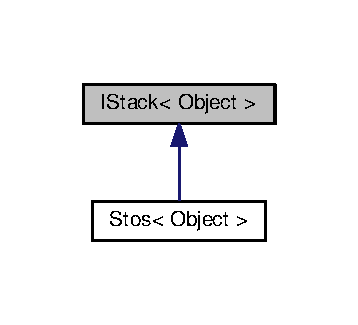
\includegraphics[width=172pt]{class_i_stack__inherit__graph}
\end{center}
\end{figure}
\subsubsection*{Metody publiczne}
\begin{DoxyCompactItemize}
\item 
virtual bool \hyperlink{class_i_stack_a5f897eeae7852113a299787faceda2c6}{Is\-Empty} ()=0
\begin{DoxyCompactList}\small\item\em Metoda sprawdzająca, czy stos jest pusty. \end{DoxyCompactList}\item 
virtual int \hyperlink{class_i_stack_a4d003c4795b2335a9038fd988875d72e}{Size} ()=0
\begin{DoxyCompactList}\small\item\em Metoda obliczająca rozmiar stosu. \end{DoxyCompactList}\item 
virtual Object \hyperlink{class_i_stack_a25ec1b2c853e59e4ec05a0579bf817ff}{Top} ()=0
\begin{DoxyCompactList}\small\item\em Metoda zwracająca wierzchołek stosu. \end{DoxyCompactList}\item 
virtual void \hyperlink{class_i_stack_a94d298580de241fd145689925a101fb1}{Push} (Object item)=0
\begin{DoxyCompactList}\small\item\em Metoda dodająca element na stos. \end{DoxyCompactList}\item 
virtual Object \hyperlink{class_i_stack_a09d0e8878c0c2c14c7f124f41786512f}{Pop} ()=0
\begin{DoxyCompactList}\small\item\em Metoda zrzucająca element ze stosu. \end{DoxyCompactList}\end{DoxyCompactItemize}


\subsubsection{Opis szczegółowy}
\subsubsection*{template$<$typename Object$>$class I\-Stack$<$ Object $>$}

Klasa szablonowa modelująca interfejs stosu. 

Definiuje A\-D\-T dla stosu.

\hyperlink{class_stos}{Stos} może przechowywać dowolny typ danych dzięki zastosowaniu szablonu. 

Definicja w linii 22 pliku I\-Stack.\-hh.



\subsubsection{Dokumentacja funkcji składowych}
\hypertarget{class_i_stack_a5f897eeae7852113a299787faceda2c6}{\index{I\-Stack@{I\-Stack}!Is\-Empty@{Is\-Empty}}
\index{Is\-Empty@{Is\-Empty}!IStack@{I\-Stack}}
\paragraph[{Is\-Empty}]{\setlength{\rightskip}{0pt plus 5cm}template$<$typename Object $>$ virtual bool {\bf I\-Stack}$<$ Object $>$\-::Is\-Empty (
\begin{DoxyParamCaption}
{}
\end{DoxyParamCaption}
)\hspace{0.3cm}{\ttfamily [pure virtual]}}}\label{class_i_stack_a5f897eeae7852113a299787faceda2c6}


Metoda sprawdzająca, czy stos jest pusty. 

true -\/ jeśli stos jest pustay  false -\/ jeśli stos nie jest pusty 

Implementowany w \hyperlink{class_stos_abc1fbf4ecba79d7d88e6f80e069315f5}{Stos$<$ Object $>$}.

\hypertarget{class_i_stack_a09d0e8878c0c2c14c7f124f41786512f}{\index{I\-Stack@{I\-Stack}!Pop@{Pop}}
\index{Pop@{Pop}!IStack@{I\-Stack}}
\paragraph[{Pop}]{\setlength{\rightskip}{0pt plus 5cm}template$<$typename Object $>$ virtual Object {\bf I\-Stack}$<$ Object $>$\-::Pop (
\begin{DoxyParamCaption}
{}
\end{DoxyParamCaption}
)\hspace{0.3cm}{\ttfamily [pure virtual]}}}\label{class_i_stack_a09d0e8878c0c2c14c7f124f41786512f}


Metoda zrzucająca element ze stosu. 

Usuwa wierzchołek ze stosu i zwraca jego wartość. \begin{DoxyReturn}{Zwraca}
element na wierzchu stosu 
\end{DoxyReturn}


Implementowany w \hyperlink{class_stos_aa4b761d3581113ee3cf312a501ed115a}{Stos$<$ Object $>$}.

\hypertarget{class_i_stack_a94d298580de241fd145689925a101fb1}{\index{I\-Stack@{I\-Stack}!Push@{Push}}
\index{Push@{Push}!IStack@{I\-Stack}}
\paragraph[{Push}]{\setlength{\rightskip}{0pt plus 5cm}template$<$typename Object $>$ virtual void {\bf I\-Stack}$<$ Object $>$\-::Push (
\begin{DoxyParamCaption}
\item[{Object}]{item}
\end{DoxyParamCaption}
)\hspace{0.3cm}{\ttfamily [pure virtual]}}}\label{class_i_stack_a94d298580de241fd145689925a101fb1}


Metoda dodająca element na stos. 

Wrzuca element na wierzchołek stosu. 
\begin{DoxyParams}[1]{Parametry}
\mbox{\tt in}  & {\em item} & -\/ element do dodania \\
\hline
\end{DoxyParams}


Implementowany w \hyperlink{class_stos_aa149141113dd5b156f21518a9a1e6c8e}{Stos$<$ Object $>$}.

\hypertarget{class_i_stack_a4d003c4795b2335a9038fd988875d72e}{\index{I\-Stack@{I\-Stack}!Size@{Size}}
\index{Size@{Size}!IStack@{I\-Stack}}
\paragraph[{Size}]{\setlength{\rightskip}{0pt plus 5cm}template$<$typename Object $>$ virtual int {\bf I\-Stack}$<$ Object $>$\-::Size (
\begin{DoxyParamCaption}
{}
\end{DoxyParamCaption}
)\hspace{0.3cm}{\ttfamily [pure virtual]}}}\label{class_i_stack_a4d003c4795b2335a9038fd988875d72e}


Metoda obliczająca rozmiar stosu. 

\begin{DoxyReturn}{Zwraca}
liczba elementów na stos 
\end{DoxyReturn}


Implementowany w \hyperlink{class_stos_a54058e5bf9a0f981cbc82f7cb130f565}{Stos$<$ Object $>$}.

\hypertarget{class_i_stack_a25ec1b2c853e59e4ec05a0579bf817ff}{\index{I\-Stack@{I\-Stack}!Top@{Top}}
\index{Top@{Top}!IStack@{I\-Stack}}
\paragraph[{Top}]{\setlength{\rightskip}{0pt plus 5cm}template$<$typename Object $>$ virtual Object {\bf I\-Stack}$<$ Object $>$\-::Top (
\begin{DoxyParamCaption}
{}
\end{DoxyParamCaption}
)\hspace{0.3cm}{\ttfamily [pure virtual]}}}\label{class_i_stack_a25ec1b2c853e59e4ec05a0579bf817ff}


Metoda zwracająca wierzchołek stosu. 

\begin{DoxyReturn}{Zwraca}
element na wierzchu stosu 
\end{DoxyReturn}


Implementowany w \hyperlink{class_stos_af7be7c7dd2e137e619c8497025119ad5}{Stos$<$ Object $>$}.



Dokumentacja dla tej klasy została wygenerowana z pliku\-:\begin{DoxyCompactItemize}
\item 
prj/inc/\hyperlink{_i_stack_8hh}{I\-Stack.\-hh}\end{DoxyCompactItemize}

\hypertarget{class_kolejka}{\subsection{Dokumentacja szablonu klasy Kolejka$<$ Object $>$}
\label{class_kolejka}\index{Kolejka$<$ Object $>$@{Kolejka$<$ Object $>$}}
}


Klasa szablonowa implementująca kolejkę  




{\ttfamily \#include $<$Kolejka.\-hh$>$}



Diagram dziedziczenia dla Kolejka$<$ Object $>$
\nopagebreak
\begin{figure}[H]
\begin{center}
\leavevmode
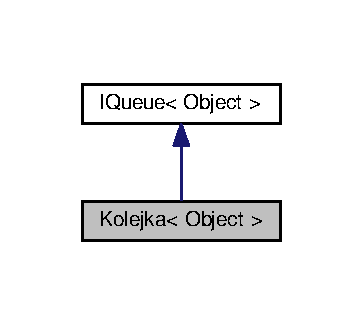
\includegraphics[width=174pt]{class_kolejka__inherit__graph}
\end{center}
\end{figure}


Diagram współpracy dla Kolejka$<$ Object $>$\-:
\nopagebreak
\begin{figure}[H]
\begin{center}
\leavevmode
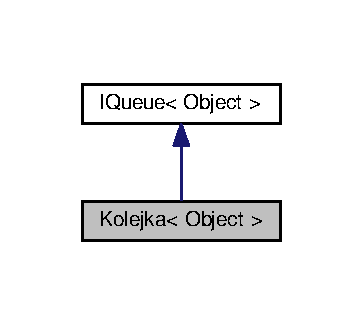
\includegraphics[width=174pt]{class_kolejka__coll__graph}
\end{center}
\end{figure}
\subsubsection*{Metody publiczne}
\begin{DoxyCompactItemize}
\item 
\hyperlink{class_kolejka_acba6bee79d22a4e0de01f1ad169d3889}{Kolejka} ()
\begin{DoxyCompactList}\small\item\em Konstruktor bezargumentowy kolejki. \end{DoxyCompactList}\item 
\hyperlink{class_kolejka_a145c1e99eea786ec7832bdc467048a2d}{$\sim$\-Kolejka} ()
\begin{DoxyCompactList}\small\item\em Destruktor kolejki. \end{DoxyCompactList}\item 
virtual bool \hyperlink{class_kolejka_a15a8e2eff269ee2d6264af30cfd23cb2}{Is\-Empty} ()
\begin{DoxyCompactList}\small\item\em Metoda sprawdzająca, czy kolejka jest pusta. \end{DoxyCompactList}\item 
virtual Object \hyperlink{class_kolejka_a04e41ef06540e8a5f5338da175f26a1f}{Front} ()
\begin{DoxyCompactList}\small\item\em Metoda zwracająca pierwszy element kolejki. \end{DoxyCompactList}\item 
virtual void \hyperlink{class_kolejka_a726ad18814137293bfdfd0500da27038}{Enqueue} (Object item)
\begin{DoxyCompactList}\small\item\em Metoda dodająca element do kolejki. \end{DoxyCompactList}\item 
virtual Object \hyperlink{class_kolejka_a61f6ec1436c1e95ce8675c8ccaf3e469}{Dequeue} ()
\begin{DoxyCompactList}\small\item\em Metoda usuwająca element kolejki. \end{DoxyCompactList}\end{DoxyCompactItemize}


\subsubsection{Opis szczegółowy}
\subsubsection*{template$<$typename Object$>$class Kolejka$<$ Object $>$}

Klasa szablonowa implementująca kolejkę 

\hyperlink{class_kolejka}{Kolejka} zbudowana jest w oparciu o dynamiczną tablicę.

\hyperlink{class_kolejka}{Kolejka} może przechowywać dowolny typ danych dzięki zastosowaniu szablonu. 

Definicja w linii 24 pliku Kolejka.\-hh.



\subsubsection{Dokumentacja konstruktora i destruktora}
\hypertarget{class_kolejka_acba6bee79d22a4e0de01f1ad169d3889}{\index{Kolejka@{Kolejka}!Kolejka@{Kolejka}}
\index{Kolejka@{Kolejka}!Kolejka@{Kolejka}}
\paragraph[{Kolejka}]{\setlength{\rightskip}{0pt plus 5cm}template$<$typename Object $>$ {\bf Kolejka}$<$ Object $>$\-::{\bf Kolejka} (
\begin{DoxyParamCaption}
{}
\end{DoxyParamCaption}
)}}\label{class_kolejka_acba6bee79d22a4e0de01f1ad169d3889}


Konstruktor bezargumentowy kolejki. 

Inicjuje Kolejkę poprzez zaalokowanie tablicy o rozmiarze 1. Ustawia indeksy f (front) i r (rear) na 0. 

Definicja w linii 90 pliku Kolejka.\-hh.

\hypertarget{class_kolejka_a145c1e99eea786ec7832bdc467048a2d}{\index{Kolejka@{Kolejka}!$\sim$\-Kolejka@{$\sim$\-Kolejka}}
\index{$\sim$\-Kolejka@{$\sim$\-Kolejka}!Kolejka@{Kolejka}}
\paragraph[{$\sim$\-Kolejka}]{\setlength{\rightskip}{0pt plus 5cm}template$<$typename Object $>$ {\bf Kolejka}$<$ Object $>$\-::$\sim${\bf Kolejka} (
\begin{DoxyParamCaption}
{}
\end{DoxyParamCaption}
)}}\label{class_kolejka_a145c1e99eea786ec7832bdc467048a2d}


Destruktor kolejki. 

Zwalnia pamięć zajmowaną przez kolejkę. Ustawia wskaźnik tablicy na N\-U\-L\-L. 

Definicja w linii 96 pliku Kolejka.\-hh.



\subsubsection{Dokumentacja funkcji składowych}
\hypertarget{class_kolejka_a61f6ec1436c1e95ce8675c8ccaf3e469}{\index{Kolejka@{Kolejka}!Dequeue@{Dequeue}}
\index{Dequeue@{Dequeue}!Kolejka@{Kolejka}}
\paragraph[{Dequeue}]{\setlength{\rightskip}{0pt plus 5cm}template$<$typename Object $>$ Object {\bf Kolejka}$<$ Object $>$\-::Dequeue (
\begin{DoxyParamCaption}
{}
\end{DoxyParamCaption}
)\hspace{0.3cm}{\ttfamily [virtual]}}}\label{class_kolejka_a61f6ec1436c1e95ce8675c8ccaf3e469}


Metoda usuwająca element kolejki. 

Sprawdza, czy kolejka jest pusta. Jeśli tak, wyrzuca wyjątek. Jeśli nie, usuwa element z początki kolejki o indeksie f (front), a następnie przesuwa indeks f o jedno miejsce dalej. \begin{DoxyReturn}{Zwraca}
pierwszy element kolejki 
\end{DoxyReturn}


Implementuje \hyperlink{class_i_queue_a6836f64bdf7102fdda590f21f7e5e208}{I\-Queue$<$ Object $>$}.



Definicja w linii 131 pliku Kolejka.\-hh.

\hypertarget{class_kolejka_a726ad18814137293bfdfd0500da27038}{\index{Kolejka@{Kolejka}!Enqueue@{Enqueue}}
\index{Enqueue@{Enqueue}!Kolejka@{Kolejka}}
\paragraph[{Enqueue}]{\setlength{\rightskip}{0pt plus 5cm}template$<$typename Object $>$ void {\bf Kolejka}$<$ Object $>$\-::Enqueue (
\begin{DoxyParamCaption}
\item[{Object}]{item}
\end{DoxyParamCaption}
)\hspace{0.3cm}{\ttfamily [virtual]}}}\label{class_kolejka_a726ad18814137293bfdfd0500da27038}


Metoda dodająca element do kolejki. 

Ustawia element na koniec kolejki
\begin{DoxyItemize}
\item komórka tablicy o indeksie r (rear). Jeśli nie ma już miejsca w kolejce tablica jest powiększana 2 razy. Następnie element zostaje prawidłowo dodany do kolejki, a indeks r zostaje przesunięty o jedno miejsce dalej. 
\begin{DoxyParams}[1]{Parametry}
\mbox{\tt in}  & {\em item} & -\/ element do dodania \\
\hline
\end{DoxyParams}

\end{DoxyItemize}

Implementuje \hyperlink{class_i_queue_af818d0fb70a5d088e6088c42f51df7e1}{I\-Queue$<$ Object $>$}.



Definicja w linii 118 pliku Kolejka.\-hh.

\hypertarget{class_kolejka_a04e41ef06540e8a5f5338da175f26a1f}{\index{Kolejka@{Kolejka}!Front@{Front}}
\index{Front@{Front}!Kolejka@{Kolejka}}
\paragraph[{Front}]{\setlength{\rightskip}{0pt plus 5cm}template$<$typename Object $>$ Object {\bf Kolejka}$<$ Object $>$\-::Front (
\begin{DoxyParamCaption}
{}
\end{DoxyParamCaption}
)\hspace{0.3cm}{\ttfamily [virtual]}}}\label{class_kolejka_a04e41ef06540e8a5f5338da175f26a1f}


Metoda zwracająca pierwszy element kolejki. 

Jeśli kolejka jest pusta, wyrzuca wyjątek. Zwraca element tablicy o indeksie f (front). \begin{DoxyReturn}{Zwraca}
pierwszy element kolejki 
\end{DoxyReturn}


Implementuje \hyperlink{class_i_queue_ab07e072ad92e4e93d57a0d3950c72764}{I\-Queue$<$ Object $>$}.



Definicja w linii 109 pliku Kolejka.\-hh.

\hypertarget{class_kolejka_a15a8e2eff269ee2d6264af30cfd23cb2}{\index{Kolejka@{Kolejka}!Is\-Empty@{Is\-Empty}}
\index{Is\-Empty@{Is\-Empty}!Kolejka@{Kolejka}}
\paragraph[{Is\-Empty}]{\setlength{\rightskip}{0pt plus 5cm}template$<$typename Object $>$ bool {\bf Kolejka}$<$ Object $>$\-::Is\-Empty (
\begin{DoxyParamCaption}
{}
\end{DoxyParamCaption}
)\hspace{0.3cm}{\ttfamily [virtual]}}}\label{class_kolejka_a15a8e2eff269ee2d6264af30cfd23cb2}


Metoda sprawdzająca, czy kolejka jest pusta. 

\hyperlink{class_kolejka}{Kolejka} jest pusta, jeśli wartości indeksów f (front) i r (rear) są sobie równe.  true -\/ jeśli lista jest pusta  false -\/ jeśli nie jest pusta 

Implementuje \hyperlink{class_i_queue_ae1c9e42be6ff647666c4468d3eec55a1}{I\-Queue$<$ Object $>$}.



Definicja w linii 103 pliku Kolejka.\-hh.



Dokumentacja dla tej klasy została wygenerowana z pliku\-:\begin{DoxyCompactItemize}
\item 
prj/inc/\hyperlink{_kolejka_8hh}{Kolejka.\-hh}\end{DoxyCompactItemize}

\hypertarget{class_s_node}{\subsection{Dokumentacja szablonu klasy S\-Node$<$ Object $>$}
\label{class_s_node}\index{S\-Node$<$ Object $>$@{S\-Node$<$ Object $>$}}
}


{\ttfamily \#include $<$S\-Node.\-hh$>$}

\subsubsection*{Metody publiczne}
\begin{DoxyCompactItemize}
\item 
\hyperlink{class_s_node_ab14f50f6fd59a6153060ac86d5278468}{S\-Node} ()
\item 
Object \hyperlink{class_s_node_a54d578a4676d559cbb695a429307927b}{Get\-Element} ()
\item 
\hyperlink{class_s_node}{S\-Node}$<$ Object $>$ $\ast$ \hyperlink{class_s_node_aa1c6c837ee647ced10147d708e10adb4}{Get\-Next} ()
\item 
void \hyperlink{class_s_node_ab78cdd2a802841b362c54f669cab8ac4}{Set\-Element} (Object new\-Item)
\item 
void \hyperlink{class_s_node_a861447eb735779a0109f9c8c0650acb5}{Set\-Next} (\hyperlink{class_s_node}{S\-Node}$<$ Object $>$ $\ast$new\-Item)
\end{DoxyCompactItemize}


\subsubsection{Opis szczegółowy}
\subsubsection*{template$<$typename Object$>$class S\-Node$<$ Object $>$}



Definicja w linii 8 pliku S\-Node.\-hh.



\subsubsection{Dokumentacja konstruktora i destruktora}
\hypertarget{class_s_node_ab14f50f6fd59a6153060ac86d5278468}{\index{S\-Node@{S\-Node}!S\-Node@{S\-Node}}
\index{S\-Node@{S\-Node}!SNode@{S\-Node}}
\paragraph[{S\-Node}]{\setlength{\rightskip}{0pt plus 5cm}template$<$typename Object$>$ {\bf S\-Node}$<$ Object $>$\-::{\bf S\-Node} (
\begin{DoxyParamCaption}
{}
\end{DoxyParamCaption}
)\hspace{0.3cm}{\ttfamily [inline]}}}\label{class_s_node_ab14f50f6fd59a6153060ac86d5278468}


Definicja w linii 14 pliku S\-Node.\-hh.



\subsubsection{Dokumentacja funkcji składowych}
\hypertarget{class_s_node_a54d578a4676d559cbb695a429307927b}{\index{S\-Node@{S\-Node}!Get\-Element@{Get\-Element}}
\index{Get\-Element@{Get\-Element}!SNode@{S\-Node}}
\paragraph[{Get\-Element}]{\setlength{\rightskip}{0pt plus 5cm}template$<$typename Object$>$ Object {\bf S\-Node}$<$ Object $>$\-::Get\-Element (
\begin{DoxyParamCaption}
{}
\end{DoxyParamCaption}
)\hspace{0.3cm}{\ttfamily [inline]}}}\label{class_s_node_a54d578a4676d559cbb695a429307927b}


Definicja w linii 15 pliku S\-Node.\-hh.

\hypertarget{class_s_node_aa1c6c837ee647ced10147d708e10adb4}{\index{S\-Node@{S\-Node}!Get\-Next@{Get\-Next}}
\index{Get\-Next@{Get\-Next}!SNode@{S\-Node}}
\paragraph[{Get\-Next}]{\setlength{\rightskip}{0pt plus 5cm}template$<$typename Object$>$ {\bf S\-Node}$<$Object$>$$\ast$ {\bf S\-Node}$<$ Object $>$\-::Get\-Next (
\begin{DoxyParamCaption}
{}
\end{DoxyParamCaption}
)\hspace{0.3cm}{\ttfamily [inline]}}}\label{class_s_node_aa1c6c837ee647ced10147d708e10adb4}


Definicja w linii 16 pliku S\-Node.\-hh.

\hypertarget{class_s_node_ab78cdd2a802841b362c54f669cab8ac4}{\index{S\-Node@{S\-Node}!Set\-Element@{Set\-Element}}
\index{Set\-Element@{Set\-Element}!SNode@{S\-Node}}
\paragraph[{Set\-Element}]{\setlength{\rightskip}{0pt plus 5cm}template$<$typename Object$>$ void {\bf S\-Node}$<$ Object $>$\-::Set\-Element (
\begin{DoxyParamCaption}
\item[{Object}]{new\-Item}
\end{DoxyParamCaption}
)\hspace{0.3cm}{\ttfamily [inline]}}}\label{class_s_node_ab78cdd2a802841b362c54f669cab8ac4}


Definicja w linii 17 pliku S\-Node.\-hh.

\hypertarget{class_s_node_a861447eb735779a0109f9c8c0650acb5}{\index{S\-Node@{S\-Node}!Set\-Next@{Set\-Next}}
\index{Set\-Next@{Set\-Next}!SNode@{S\-Node}}
\paragraph[{Set\-Next}]{\setlength{\rightskip}{0pt plus 5cm}template$<$typename Object$>$ void {\bf S\-Node}$<$ Object $>$\-::Set\-Next (
\begin{DoxyParamCaption}
\item[{{\bf S\-Node}$<$ Object $>$ $\ast$}]{new\-Item}
\end{DoxyParamCaption}
)\hspace{0.3cm}{\ttfamily [inline]}}}\label{class_s_node_a861447eb735779a0109f9c8c0650acb5}


Definicja w linii 18 pliku S\-Node.\-hh.



Dokumentacja dla tej klasy została wygenerowana z pliku\-:\begin{DoxyCompactItemize}
\item 
prj/inc/\hyperlink{_s_node_8hh}{S\-Node.\-hh}\end{DoxyCompactItemize}

\hypertarget{class_stopwatch}{\subsection{Dokumentacja klasy Stopwatch}
\label{class_stopwatch}\index{Stopwatch@{Stopwatch}}
}


Klasa implementująca podstawowy stoper.  




{\ttfamily \#include $<$Stopwatch.\-hh$>$}



Diagram dziedziczenia dla Stopwatch
\nopagebreak
\begin{figure}[H]
\begin{center}
\leavevmode
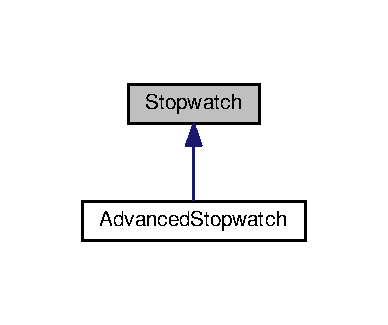
\includegraphics[width=186pt]{class_stopwatch__inherit__graph}
\end{center}
\end{figure}
\subsubsection*{Metody publiczne}
\begin{DoxyCompactItemize}
\item 
virtual void \hyperlink{class_stopwatch_adb93923510f12409132445fc187d828f}{Start} ()
\begin{DoxyCompactList}\small\item\em Rozpoczyna pomiar czasu. \end{DoxyCompactList}\item 
virtual void \hyperlink{class_stopwatch_afb2754584ef39767d8182f2345cd9721}{Stop} ()
\begin{DoxyCompactList}\small\item\em Kończy pomiar czasu. \end{DoxyCompactList}\item 
virtual double \hyperlink{class_stopwatch_a65647fd3b6337c9d0c109e0b1ad293ea}{Get\-Elapsed\-Time} ()
\begin{DoxyCompactList}\small\item\em Oblicza czas na podstawie pól klasy. \end{DoxyCompactList}\end{DoxyCompactItemize}
\subsubsection*{Atrybuty chronione}
\begin{DoxyCompactItemize}
\item 
timeval \hyperlink{class_stopwatch_ac10760e0e0c54d4bdfbdb3dd9d4abb91}{start}
\item 
timeval \hyperlink{class_stopwatch_a3eb80a36c7adb793287c8858642014bc}{stop}
\end{DoxyCompactItemize}


\subsubsection{Opis szczegółowy}
Klasa implementująca podstawowy stoper. 

Klasa jest modelelem stopera z funkcjami start, stop i oblicz czas. 

Definicja w linii 20 pliku Stopwatch.\-hh.



\subsubsection{Dokumentacja funkcji składowych}
\hypertarget{class_stopwatch_a65647fd3b6337c9d0c109e0b1ad293ea}{\index{Stopwatch@{Stopwatch}!Get\-Elapsed\-Time@{Get\-Elapsed\-Time}}
\index{Get\-Elapsed\-Time@{Get\-Elapsed\-Time}!Stopwatch@{Stopwatch}}
\paragraph[{Get\-Elapsed\-Time}]{\setlength{\rightskip}{0pt plus 5cm}double Stopwatch\-::\-Get\-Elapsed\-Time (
\begin{DoxyParamCaption}
{}
\end{DoxyParamCaption}
)\hspace{0.3cm}{\ttfamily [virtual]}}}\label{class_stopwatch_a65647fd3b6337c9d0c109e0b1ad293ea}


Oblicza czas na podstawie pól klasy. 

Odejmuje wartości zapisane w polach stop i start. Daje wynik w mikrosekundach. 

Definicja w linii 12 pliku Stopwatch.\-cpp.

\hypertarget{class_stopwatch_adb93923510f12409132445fc187d828f}{\index{Stopwatch@{Stopwatch}!Start@{Start}}
\index{Start@{Start}!Stopwatch@{Stopwatch}}
\paragraph[{Start}]{\setlength{\rightskip}{0pt plus 5cm}void Stopwatch\-::\-Start (
\begin{DoxyParamCaption}
{}
\end{DoxyParamCaption}
)\hspace{0.3cm}{\ttfamily [virtual]}}}\label{class_stopwatch_adb93923510f12409132445fc187d828f}


Rozpoczyna pomiar czasu. 

Przypisuje wynik metody gettimeofday() do pola start. 

Definicja w linii 4 pliku Stopwatch.\-cpp.

\hypertarget{class_stopwatch_afb2754584ef39767d8182f2345cd9721}{\index{Stopwatch@{Stopwatch}!Stop@{Stop}}
\index{Stop@{Stop}!Stopwatch@{Stopwatch}}
\paragraph[{Stop}]{\setlength{\rightskip}{0pt plus 5cm}void Stopwatch\-::\-Stop (
\begin{DoxyParamCaption}
{}
\end{DoxyParamCaption}
)\hspace{0.3cm}{\ttfamily [virtual]}}}\label{class_stopwatch_afb2754584ef39767d8182f2345cd9721}


Kończy pomiar czasu. 

Przypisuje wynik metody gettimeofday() do pola stop. 

Definicja w linii 8 pliku Stopwatch.\-cpp.



\subsubsection{Dokumentacja atrybutów składowych}
\hypertarget{class_stopwatch_ac10760e0e0c54d4bdfbdb3dd9d4abb91}{\index{Stopwatch@{Stopwatch}!start@{start}}
\index{start@{start}!Stopwatch@{Stopwatch}}
\paragraph[{start}]{\setlength{\rightskip}{0pt plus 5cm}timeval Stopwatch\-::start\hspace{0.3cm}{\ttfamily [protected]}}}\label{class_stopwatch_ac10760e0e0c54d4bdfbdb3dd9d4abb91}


Definicja w linii 23 pliku Stopwatch.\-hh.

\hypertarget{class_stopwatch_a3eb80a36c7adb793287c8858642014bc}{\index{Stopwatch@{Stopwatch}!stop@{stop}}
\index{stop@{stop}!Stopwatch@{Stopwatch}}
\paragraph[{stop}]{\setlength{\rightskip}{0pt plus 5cm}timeval Stopwatch\-::stop\hspace{0.3cm}{\ttfamily [protected]}}}\label{class_stopwatch_a3eb80a36c7adb793287c8858642014bc}
struktury timeval start i stop 

Definicja w linii 23 pliku Stopwatch.\-hh.



Dokumentacja dla tej klasy została wygenerowana z plików\-:\begin{DoxyCompactItemize}
\item 
prj/inc/\hyperlink{_stopwatch_8hh}{Stopwatch.\-hh}\item 
prj/src/\hyperlink{_stopwatch_8cpp}{Stopwatch.\-cpp}\end{DoxyCompactItemize}

\hypertarget{class_stos}{\subsection{Dokumentacja szablonu klasy Stos$<$ Object $>$}
\label{class_stos}\index{Stos$<$ Object $>$@{Stos$<$ Object $>$}}
}


Klasa szablonowa implementująca stos.  




{\ttfamily \#include $<$Stos.\-hh$>$}



Diagram dziedziczenia dla Stos$<$ Object $>$
\nopagebreak
\begin{figure}[H]
\begin{center}
\leavevmode
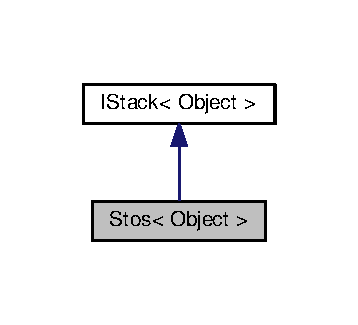
\includegraphics[width=172pt]{class_stos__inherit__graph}
\end{center}
\end{figure}


Diagram współpracy dla Stos$<$ Object $>$\-:
\nopagebreak
\begin{figure}[H]
\begin{center}
\leavevmode
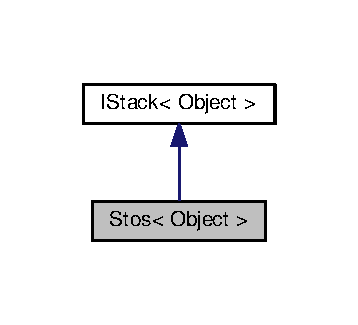
\includegraphics[width=172pt]{class_stos__coll__graph}
\end{center}
\end{figure}
\subsubsection*{Metody publiczne}
\begin{DoxyCompactItemize}
\item 
\hyperlink{class_stos_aeeaa5309f8451f8eb81c85a6ffe158c8}{Stos} ()
\begin{DoxyCompactList}\small\item\em Konstruktor bezargumentowy stosu. \end{DoxyCompactList}\item 
\hyperlink{class_stos_a008cbd24801097067a5c8c5c447ea860}{Stos} (int ile)
\begin{DoxyCompactList}\small\item\em Konstruktor stosu. \end{DoxyCompactList}\item 
\hyperlink{class_stos_a8ff945301446bcebb9538efc395499bc}{$\sim$\-Stos} ()
\begin{DoxyCompactList}\small\item\em Destruktor stosu. \end{DoxyCompactList}\item 
int \& \hyperlink{class_stos_a1ea728d6c770ffa6b06cf74d1d0ac78f}{Pojemnosc} ()
\begin{DoxyCompactList}\small\item\em Metoda sprawdzająca pojemność stosu. \end{DoxyCompactList}\item 
virtual bool \hyperlink{class_stos_abc1fbf4ecba79d7d88e6f80e069315f5}{Is\-Empty} ()
\begin{DoxyCompactList}\small\item\em Metoda sprawdzająca, czy stos jest pusty. \end{DoxyCompactList}\item 
virtual int \hyperlink{class_stos_a54058e5bf9a0f981cbc82f7cb130f565}{Size} ()
\begin{DoxyCompactList}\small\item\em Metoda obliczająca rozmiar stosu. \end{DoxyCompactList}\item 
virtual Object \hyperlink{class_stos_af7be7c7dd2e137e619c8497025119ad5}{Top} ()
\begin{DoxyCompactList}\small\item\em Metoda zwracająca wierzchołek stosu. \end{DoxyCompactList}\item 
virtual void \hyperlink{class_stos_aa149141113dd5b156f21518a9a1e6c8e}{Push} (Object item)
\begin{DoxyCompactList}\small\item\em Metoda dodająca element na stos. \end{DoxyCompactList}\item 
virtual Object \hyperlink{class_stos_aa4b761d3581113ee3cf312a501ed115a}{Pop} ()
\begin{DoxyCompactList}\small\item\em Metoda zrzucająca element ze stosu. \end{DoxyCompactList}\end{DoxyCompactItemize}


\subsubsection{Opis szczegółowy}
\subsubsection*{template$<$typename Object$>$class Stos$<$ Object $>$}

Klasa szablonowa implementująca stos. 

\hyperlink{class_stos}{Stos} zbudowany jest w oparciu o dynamiczną tablicę.

\hyperlink{class_stos}{Stos} może przechowywać dowolny typ danych dzięki zastosowaniu szablonu. 

Definicja w linii 22 pliku Stos.\-hh.



\subsubsection{Dokumentacja konstruktora i destruktora}
\hypertarget{class_stos_aeeaa5309f8451f8eb81c85a6ffe158c8}{\index{Stos@{Stos}!Stos@{Stos}}
\index{Stos@{Stos}!Stos@{Stos}}
\paragraph[{Stos}]{\setlength{\rightskip}{0pt plus 5cm}template$<$typename Object $>$ {\bf Stos}$<$ Object $>$\-::{\bf Stos} (
\begin{DoxyParamCaption}
{}
\end{DoxyParamCaption}
)}}\label{class_stos_aeeaa5309f8451f8eb81c85a6ffe158c8}


Konstruktor bezargumentowy stosu. 

Inicjuje stos poprzez zaalokowanie tablicy o rozmiarze 1. Ustawia indeks top na -\/1. 

Definicja w linii 119 pliku Stos.\-hh.

\hypertarget{class_stos_a008cbd24801097067a5c8c5c447ea860}{\index{Stos@{Stos}!Stos@{Stos}}
\index{Stos@{Stos}!Stos@{Stos}}
\paragraph[{Stos}]{\setlength{\rightskip}{0pt plus 5cm}template$<$typename Object $>$ {\bf Stos}$<$ Object $>$\-::{\bf Stos} (
\begin{DoxyParamCaption}
\item[{int}]{ile}
\end{DoxyParamCaption}
)}}\label{class_stos_a008cbd24801097067a5c8c5c447ea860}


Konstruktor stosu. 

Inicjuje stos poprzez zaalokowanie tablicy o rozmiarze podanym w argumencie konstruktora (o ile jest różny od 0). Ustawia indeks top na -\/1. 
\begin{DoxyParams}[1]{Parametry}
\mbox{\tt in}  & {\em ile} & -\/ początkowa pojemność kolejki; \\
\hline
\end{DoxyParams}


Definicja w linii 128 pliku Stos.\-hh.

\hypertarget{class_stos_a8ff945301446bcebb9538efc395499bc}{\index{Stos@{Stos}!$\sim$\-Stos@{$\sim$\-Stos}}
\index{$\sim$\-Stos@{$\sim$\-Stos}!Stos@{Stos}}
\paragraph[{$\sim$\-Stos}]{\setlength{\rightskip}{0pt plus 5cm}template$<$typename Object $>$ {\bf Stos}$<$ Object $>$\-::$\sim${\bf Stos} (
\begin{DoxyParamCaption}
{}
\end{DoxyParamCaption}
)}}\label{class_stos_a8ff945301446bcebb9538efc395499bc}


Destruktor stosu. 

Zwalnia pamięć zajmowaną przez stosu. Ustawia wskaźnik tablicy dynamicznej na N\-U\-L\-L. 

Definicja w linii 140 pliku Stos.\-hh.



\subsubsection{Dokumentacja funkcji składowych}
\hypertarget{class_stos_abc1fbf4ecba79d7d88e6f80e069315f5}{\index{Stos@{Stos}!Is\-Empty@{Is\-Empty}}
\index{Is\-Empty@{Is\-Empty}!Stos@{Stos}}
\paragraph[{Is\-Empty}]{\setlength{\rightskip}{0pt plus 5cm}template$<$typename Object $>$ bool {\bf Stos}$<$ Object $>$\-::Is\-Empty (
\begin{DoxyParamCaption}
{}
\end{DoxyParamCaption}
)\hspace{0.3cm}{\ttfamily [virtual]}}}\label{class_stos_abc1fbf4ecba79d7d88e6f80e069315f5}


Metoda sprawdzająca, czy stos jest pusty. 

Jeśli indeks top$<$0, stos jest pusty. W przeciwnym wypadku, stos nie jest pusty.  true -\/ jeśli stos jest pusty  false -\/ jeśli stos nie jest pusty 

Implementuje \hyperlink{class_i_stack_a5f897eeae7852113a299787faceda2c6}{I\-Stack$<$ Object $>$}.



Definicja w linii 147 pliku Stos.\-hh.

\hypertarget{class_stos_a1ea728d6c770ffa6b06cf74d1d0ac78f}{\index{Stos@{Stos}!Pojemnosc@{Pojemnosc}}
\index{Pojemnosc@{Pojemnosc}!Stos@{Stos}}
\paragraph[{Pojemnosc}]{\setlength{\rightskip}{0pt plus 5cm}template$<$typename Object$>$ int\& {\bf Stos}$<$ Object $>$\-::Pojemnosc (
\begin{DoxyParamCaption}
{}
\end{DoxyParamCaption}
)\hspace{0.3cm}{\ttfamily [inline]}}}\label{class_stos_a1ea728d6c770ffa6b06cf74d1d0ac78f}


Metoda sprawdzająca pojemność stosu. 

Zwraca parametr opisujący pojemność tablicy dynamicznej implementującej stos. \begin{DoxyReturn}{Zwraca}
pojemność stosu 
\end{DoxyReturn}


Definicja w linii 63 pliku Stos.\-hh.

\hypertarget{class_stos_aa4b761d3581113ee3cf312a501ed115a}{\index{Stos@{Stos}!Pop@{Pop}}
\index{Pop@{Pop}!Stos@{Stos}}
\paragraph[{Pop}]{\setlength{\rightskip}{0pt plus 5cm}template$<$typename Object $>$ Object {\bf Stos}$<$ Object $>$\-::Pop (
\begin{DoxyParamCaption}
{}
\end{DoxyParamCaption}
)\hspace{0.3cm}{\ttfamily [virtual]}}}\label{class_stos_aa4b761d3581113ee3cf312a501ed115a}


Metoda zrzucająca element ze stosu. 

Jeśli stos jest pusty, wyrzuca wyjątek. Zwraca element tablicy o indeksie top. Zmniejsza indeks top o 1. \begin{DoxyReturn}{Zwraca}
element na wierzchu stosu 
\end{DoxyReturn}


Implementuje \hyperlink{class_i_stack_a09d0e8878c0c2c14c7f124f41786512f}{I\-Stack$<$ Object $>$}.



Definicja w linii 193 pliku Stos.\-hh.

\hypertarget{class_stos_aa149141113dd5b156f21518a9a1e6c8e}{\index{Stos@{Stos}!Push@{Push}}
\index{Push@{Push}!Stos@{Stos}}
\paragraph[{Push}]{\setlength{\rightskip}{0pt plus 5cm}template$<$typename Object $>$ void {\bf Stos}$<$ Object $>$\-::Push (
\begin{DoxyParamCaption}
\item[{Object}]{item}
\end{DoxyParamCaption}
)\hspace{0.3cm}{\ttfamily [virtual]}}}\label{class_stos_aa149141113dd5b156f21518a9a1e6c8e}


Metoda dodająca element na stos. 

Wrzuca element na wierzchołek stosu. Indeks top zostaje przesunięty o jedno miejsce dalej. Jeśli nie ma już miejsca na stosie tablica jest powiększana 2 razy. Następnie element zostaje prawidłowo wrzucony na stos, a indeks top zostaje przesunięty o jedno miejsce dalej. 
\begin{DoxyParams}[1]{Parametry}
\mbox{\tt in}  & {\em item} & -\/ element do dodania \\
\hline
\end{DoxyParams}


Implementuje \hyperlink{class_i_stack_a94d298580de241fd145689925a101fb1}{I\-Stack$<$ Object $>$}.



Definicja w linii 175 pliku Stos.\-hh.

\hypertarget{class_stos_a54058e5bf9a0f981cbc82f7cb130f565}{\index{Stos@{Stos}!Size@{Size}}
\index{Size@{Size}!Stos@{Stos}}
\paragraph[{Size}]{\setlength{\rightskip}{0pt plus 5cm}template$<$typename Object $>$ int {\bf Stos}$<$ Object $>$\-::Size (
\begin{DoxyParamCaption}
{}
\end{DoxyParamCaption}
)\hspace{0.3cm}{\ttfamily [virtual]}}}\label{class_stos_a54058e5bf9a0f981cbc82f7cb130f565}


Metoda obliczająca rozmiar stosu. 

Rozmiar obliczany jest przez działanie 'top+1'. \begin{DoxyReturn}{Zwraca}
liczba elementów na stosie 
\end{DoxyReturn}


Implementuje \hyperlink{class_i_stack_a4d003c4795b2335a9038fd988875d72e}{I\-Stack$<$ Object $>$}.



Definicja w linii 156 pliku Stos.\-hh.

\hypertarget{class_stos_af7be7c7dd2e137e619c8497025119ad5}{\index{Stos@{Stos}!Top@{Top}}
\index{Top@{Top}!Stos@{Stos}}
\paragraph[{Top}]{\setlength{\rightskip}{0pt plus 5cm}template$<$typename Object $>$ Object {\bf Stos}$<$ Object $>$\-::Top (
\begin{DoxyParamCaption}
{}
\end{DoxyParamCaption}
)\hspace{0.3cm}{\ttfamily [virtual]}}}\label{class_stos_af7be7c7dd2e137e619c8497025119ad5}


Metoda zwracająca wierzchołek stosu. 

Jeśli stos jest pusty, wyrzuca wyjątek. Zwraca element tablicy o indeksie top. \begin{DoxyReturn}{Zwraca}
element na wierzchu stosu 
\end{DoxyReturn}


Implementuje \hyperlink{class_i_stack_a25ec1b2c853e59e4ec05a0579bf817ff}{I\-Stack$<$ Object $>$}.



Definicja w linii 164 pliku Stos.\-hh.



Dokumentacja dla tej klasy została wygenerowana z pliku\-:\begin{DoxyCompactItemize}
\item 
prj/inc/\hyperlink{_stos_8hh}{Stos.\-hh}\end{DoxyCompactItemize}

\section{Dokumentacja plików}
\hypertarget{_advanced_stopwatch_8hh}{\subsection{Dokumentacja pliku prj/inc/\-Advanced\-Stopwatch.hh}
\label{_advanced_stopwatch_8hh}\index{prj/inc/\-Advanced\-Stopwatch.\-hh@{prj/inc/\-Advanced\-Stopwatch.\-hh}}
}
{\ttfamily \#include \char`\"{}Stopwatch.\-hh\char`\"{}}\\*
{\ttfamily \#include $<$iostream$>$}\\*
{\ttfamily \#include $<$fstream$>$}\\*
{\ttfamily \#include $<$string$>$}\\*
{\ttfamily \#include $<$iomanip$>$}\\*
Wykres zależności załączania dla Advanced\-Stopwatch.\-hh\-:
\nopagebreak
\begin{figure}[H]
\begin{center}
\leavevmode
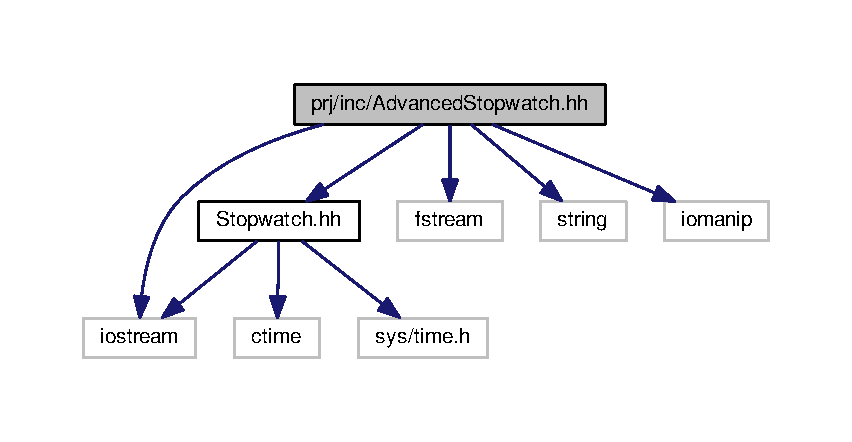
\includegraphics[width=350pt]{_advanced_stopwatch_8hh__incl}
\end{center}
\end{figure}
Ten wykres pokazuje, które pliki bezpośrednio lub pośrednio załączają ten plik\-:
\nopagebreak
\begin{figure}[H]
\begin{center}
\leavevmode
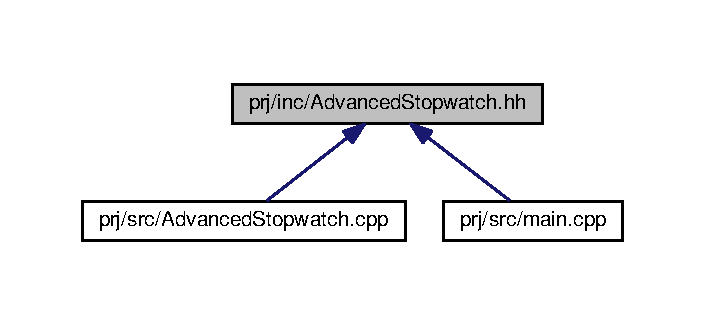
\includegraphics[width=339pt]{_advanced_stopwatch_8hh__dep__incl}
\end{center}
\end{figure}
\subsubsection*{Komponenty}
\begin{DoxyCompactItemize}
\item 
class \hyperlink{class_advanced_stopwatch}{Advanced\-Stopwatch}
\begin{DoxyCompactList}\small\item\em Klasa implementująca rozbudowany stoper. \end{DoxyCompactList}\end{DoxyCompactItemize}
\subsubsection*{Definicje}
\begin{DoxyCompactItemize}
\item 
\#define \hyperlink{_advanced_stopwatch_8hh_a77588e5ce0483d6845d1f5c362111401}{M\-A\-X\-\_\-\-L\-A\-P\-S}~100
\item 
\#define \hyperlink{_advanced_stopwatch_8hh_ab3bb2c4a1622e2f6ae128b969966e848}{B\-U\-F\-O\-R}~10
\item 
\#define \hyperlink{_advanced_stopwatch_8hh_ab44cac363b6642c6f9ba217b1d0172db}{D\-O\-K\-L\-A\-D\-N\-O\-S\-C}~8
\end{DoxyCompactItemize}


\subsubsection{Opis szczegółowy}
Plik zawiera implementację rozbudowanego stopera. 

Definicja w pliku \hyperlink{_advanced_stopwatch_8hh_source}{Advanced\-Stopwatch.\-hh}.



\subsubsection{Dokumentacja definicji}
\hypertarget{_advanced_stopwatch_8hh_ab3bb2c4a1622e2f6ae128b969966e848}{\index{Advanced\-Stopwatch.\-hh@{Advanced\-Stopwatch.\-hh}!B\-U\-F\-O\-R@{B\-U\-F\-O\-R}}
\index{B\-U\-F\-O\-R@{B\-U\-F\-O\-R}!AdvancedStopwatch.hh@{Advanced\-Stopwatch.\-hh}}
\paragraph[{B\-U\-F\-O\-R}]{\setlength{\rightskip}{0pt plus 5cm}\#define B\-U\-F\-O\-R~10}}\label{_advanced_stopwatch_8hh_ab3bb2c4a1622e2f6ae128b969966e848}


Definicja w linii 12 pliku Advanced\-Stopwatch.\-hh.

\hypertarget{_advanced_stopwatch_8hh_ab44cac363b6642c6f9ba217b1d0172db}{\index{Advanced\-Stopwatch.\-hh@{Advanced\-Stopwatch.\-hh}!D\-O\-K\-L\-A\-D\-N\-O\-S\-C@{D\-O\-K\-L\-A\-D\-N\-O\-S\-C}}
\index{D\-O\-K\-L\-A\-D\-N\-O\-S\-C@{D\-O\-K\-L\-A\-D\-N\-O\-S\-C}!AdvancedStopwatch.hh@{Advanced\-Stopwatch.\-hh}}
\paragraph[{D\-O\-K\-L\-A\-D\-N\-O\-S\-C}]{\setlength{\rightskip}{0pt plus 5cm}\#define D\-O\-K\-L\-A\-D\-N\-O\-S\-C~8}}\label{_advanced_stopwatch_8hh_ab44cac363b6642c6f9ba217b1d0172db}


Definicja w linii 13 pliku Advanced\-Stopwatch.\-hh.

\hypertarget{_advanced_stopwatch_8hh_a77588e5ce0483d6845d1f5c362111401}{\index{Advanced\-Stopwatch.\-hh@{Advanced\-Stopwatch.\-hh}!M\-A\-X\-\_\-\-L\-A\-P\-S@{M\-A\-X\-\_\-\-L\-A\-P\-S}}
\index{M\-A\-X\-\_\-\-L\-A\-P\-S@{M\-A\-X\-\_\-\-L\-A\-P\-S}!AdvancedStopwatch.hh@{Advanced\-Stopwatch.\-hh}}
\paragraph[{M\-A\-X\-\_\-\-L\-A\-P\-S}]{\setlength{\rightskip}{0pt plus 5cm}\#define M\-A\-X\-\_\-\-L\-A\-P\-S~100}}\label{_advanced_stopwatch_8hh_a77588e5ce0483d6845d1f5c362111401}


Definicja w linii 11 pliku Advanced\-Stopwatch.\-hh.


\hypertarget{_b_list_8hh}{\subsection{Dokumentacja pliku prj/inc/\-B\-List.hh}
\label{_b_list_8hh}\index{prj/inc/\-B\-List.\-hh@{prj/inc/\-B\-List.\-hh}}
}
{\ttfamily \#include $<$iostream$>$}\\*
{\ttfamily \#include \char`\"{}I\-List.\-hh\char`\"{}}\\*
{\ttfamily \#include \char`\"{}B\-Node.\-hh\char`\"{}}\\*
Wykres zależności załączania dla B\-List.\-hh\-:
\nopagebreak
\begin{figure}[H]
\begin{center}
\leavevmode
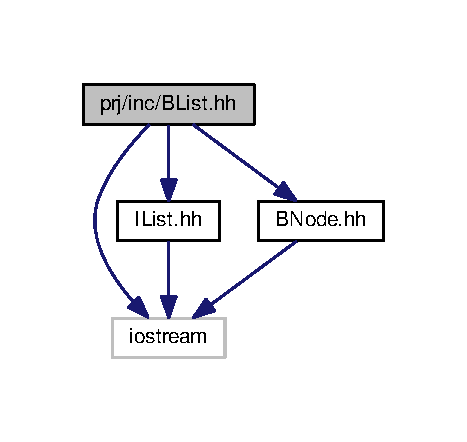
\includegraphics[width=224pt]{_b_list_8hh__incl}
\end{center}
\end{figure}
Ten wykres pokazuje, które pliki bezpośrednio lub pośrednio załączają ten plik\-:
\nopagebreak
\begin{figure}[H]
\begin{center}
\leavevmode
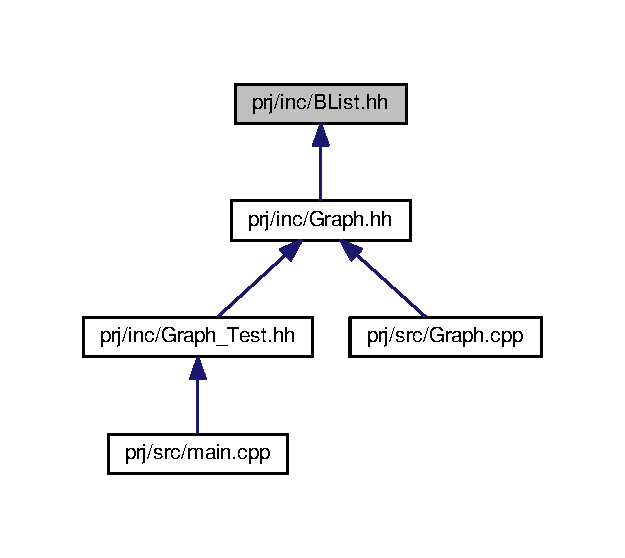
\includegraphics[width=300pt]{_b_list_8hh__dep__incl}
\end{center}
\end{figure}
\subsubsection*{Komponenty}
\begin{DoxyCompactItemize}
\item 
class \hyperlink{class_b_list}{B\-List$<$ Object $>$}
\begin{DoxyCompactList}\small\item\em Szablonowa klasa implementująca listę dwukierunkową \end{DoxyCompactList}\end{DoxyCompactItemize}


\subsubsection{Opis szczegółowy}
Plik zawiera definicję klasy implementującej listę dwukierunkową. 

Definicja w pliku \hyperlink{_b_list_8hh_source}{B\-List.\-hh}.


\hypertarget{_b_node_8hh}{\subsection{Dokumentacja pliku prj/inc/\-B\-Node.hh}
\label{_b_node_8hh}\index{prj/inc/\-B\-Node.\-hh@{prj/inc/\-B\-Node.\-hh}}
}
{\ttfamily \#include $<$iostream$>$}\\*
Wykres zależności załączania dla B\-Node.\-hh\-:
\nopagebreak
\begin{figure}[H]
\begin{center}
\leavevmode
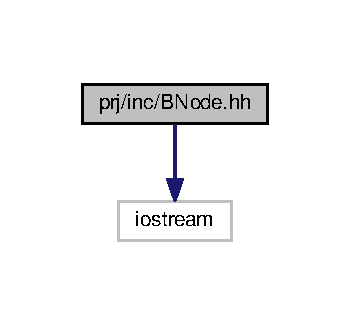
\includegraphics[width=168pt]{_b_node_8hh__incl}
\end{center}
\end{figure}
Ten wykres pokazuje, które pliki bezpośrednio lub pośrednio załączają ten plik\-:
\nopagebreak
\begin{figure}[H]
\begin{center}
\leavevmode
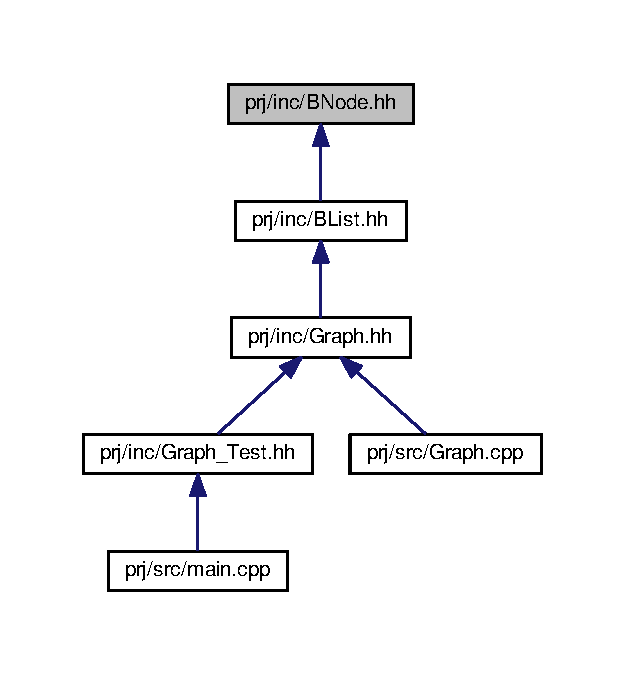
\includegraphics[width=300pt]{_b_node_8hh__dep__incl}
\end{center}
\end{figure}
\subsubsection*{Komponenty}
\begin{DoxyCompactItemize}
\item 
class \hyperlink{class_b_node}{B\-Node$<$ Object $>$}
\end{DoxyCompactItemize}

\hypertarget{_graph_8hh}{\subsection{Dokumentacja pliku prj/inc/\-Graph.hh}
\label{_graph_8hh}\index{prj/inc/\-Graph.\-hh@{prj/inc/\-Graph.\-hh}}
}
{\ttfamily \#include $<$iostream$>$}\\*
{\ttfamily \#include \char`\"{}I\-Graph.\-hh\char`\"{}}\\*
{\ttfamily \#include \char`\"{}B\-List.\-hh\char`\"{}}\\*
{\ttfamily \#include \char`\"{}Kolejka.\-hh\char`\"{}}\\*
{\ttfamily \#include \char`\"{}Stos.\-hh\char`\"{}}\\*
Wykres zależności załączania dla Graph.\-hh\-:
\nopagebreak
\begin{figure}[H]
\begin{center}
\leavevmode
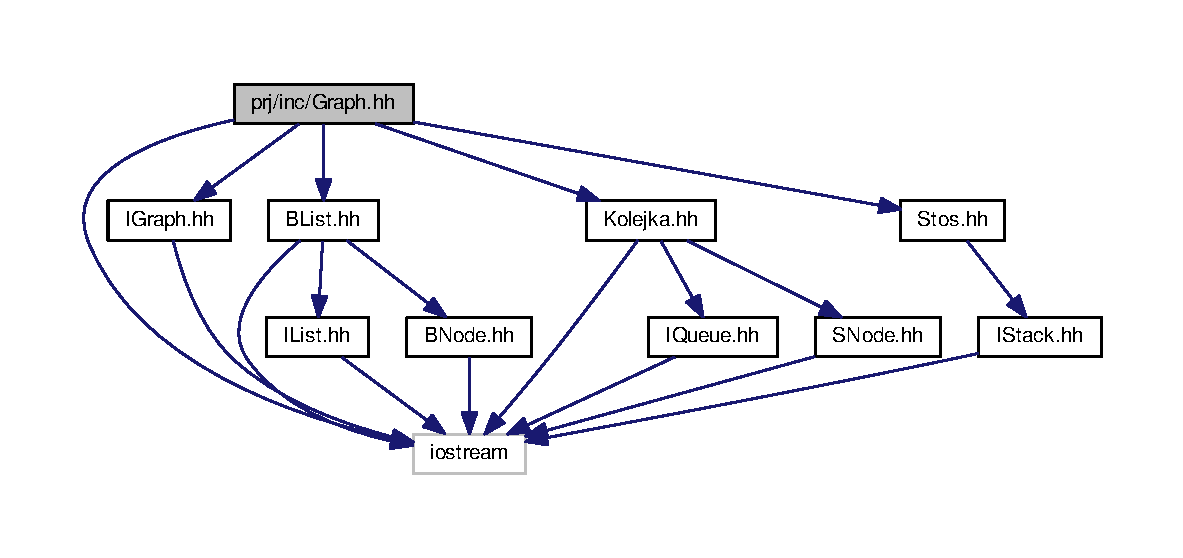
\includegraphics[width=350pt]{_graph_8hh__incl}
\end{center}
\end{figure}
Ten wykres pokazuje, które pliki bezpośrednio lub pośrednio załączają ten plik\-:
\nopagebreak
\begin{figure}[H]
\begin{center}
\leavevmode
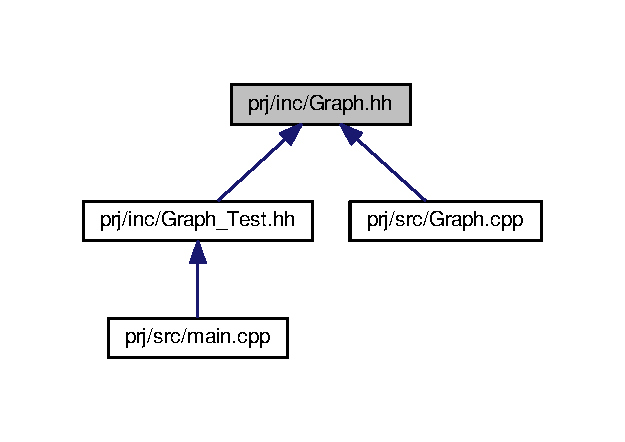
\includegraphics[width=300pt]{_graph_8hh__dep__incl}
\end{center}
\end{figure}
\subsubsection*{Komponenty}
\begin{DoxyCompactItemize}
\item 
class \hyperlink{class_graph}{Graph}
\end{DoxyCompactItemize}


\subsubsection{Opis szczegółowy}
Plik zawiera implementację interfejsu grafu. 

Definicja w pliku \hyperlink{_graph_8hh_source}{Graph.\-hh}.


\hypertarget{_graph___test_8hh}{\subsection{Dokumentacja pliku prj/inc/\-Graph\-\_\-\-Test.hh}
\label{_graph___test_8hh}\index{prj/inc/\-Graph\-\_\-\-Test.\-hh@{prj/inc/\-Graph\-\_\-\-Test.\-hh}}
}
{\ttfamily \#include $<$iostream$>$}\\*
{\ttfamily \#include \char`\"{}I\-Runnable.\-hh\char`\"{}}\\*
{\ttfamily \#include \char`\"{}Graph.\-hh\char`\"{}}\\*
Wykres zależności załączania dla Graph\-\_\-\-Test.\-hh\-:
\nopagebreak
\begin{figure}[H]
\begin{center}
\leavevmode
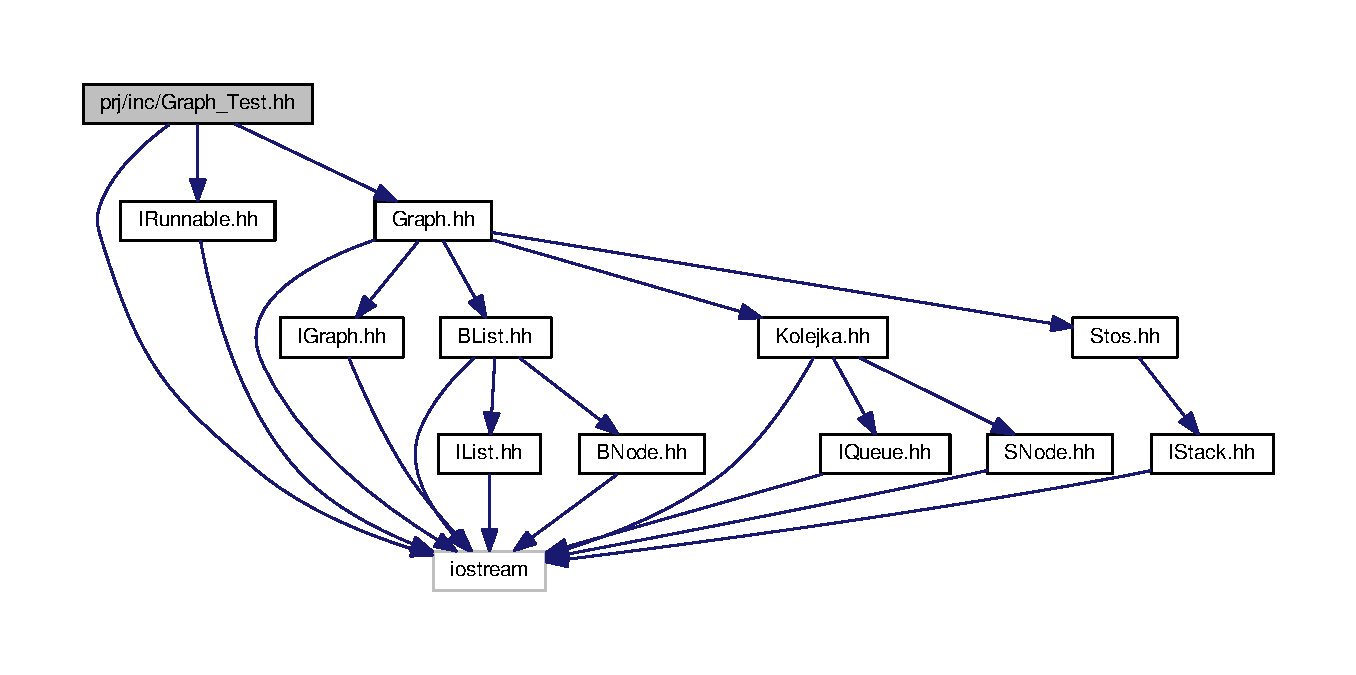
\includegraphics[width=350pt]{_graph___test_8hh__incl}
\end{center}
\end{figure}
Ten wykres pokazuje, które pliki bezpośrednio lub pośrednio załączają ten plik\-:
\nopagebreak
\begin{figure}[H]
\begin{center}
\leavevmode
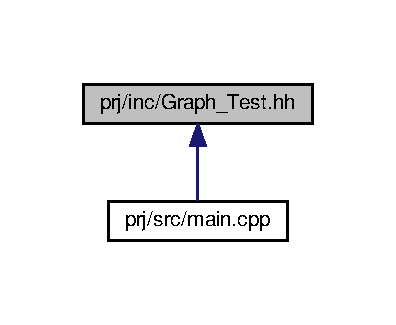
\includegraphics[width=190pt]{_graph___test_8hh__dep__incl}
\end{center}
\end{figure}
\subsubsection*{Komponenty}
\begin{DoxyCompactItemize}
\item 
class \hyperlink{class_graph___test}{Graph\-\_\-\-Test$<$ Object $>$}
\begin{DoxyCompactList}\small\item\em Szablonowa klasa implementująca testowy graf. \end{DoxyCompactList}\end{DoxyCompactItemize}


\subsubsection{Opis szczegółowy}
Plik zawiera implementację \hyperlink{class_i_runnable}{I\-Runnable} dla grafu (operacje B\-F\-S i D\-F\-S). 

Definicja w pliku \hyperlink{_graph___test_8hh_source}{Graph\-\_\-\-Test.\-hh}.


\hypertarget{_i_graph_8hh}{\subsection{Dokumentacja pliku prj/inc/\-I\-Graph.hh}
\label{_i_graph_8hh}\index{prj/inc/\-I\-Graph.\-hh@{prj/inc/\-I\-Graph.\-hh}}
}
{\ttfamily \#include $<$iostream$>$}\\*
Wykres zależności załączania dla I\-Graph.\-hh\-:
\nopagebreak
\begin{figure}[H]
\begin{center}
\leavevmode
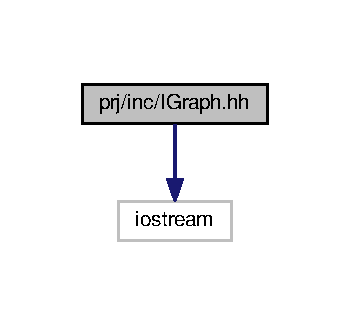
\includegraphics[width=168pt]{_i_graph_8hh__incl}
\end{center}
\end{figure}
Ten wykres pokazuje, które pliki bezpośrednio lub pośrednio załączają ten plik\-:
\nopagebreak
\begin{figure}[H]
\begin{center}
\leavevmode
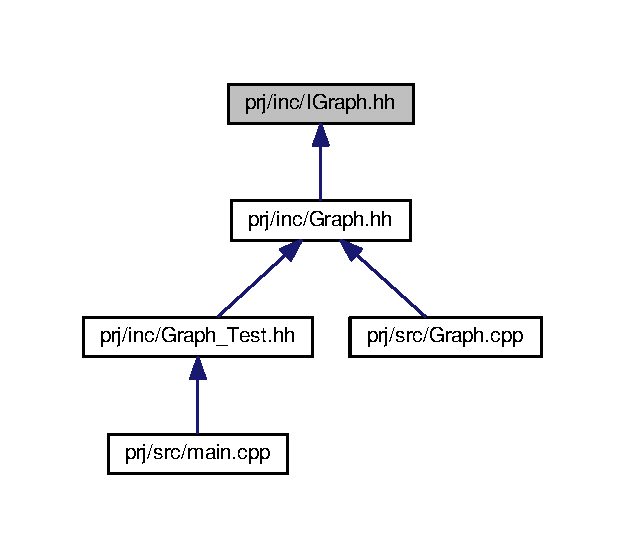
\includegraphics[width=300pt]{_i_graph_8hh__dep__incl}
\end{center}
\end{figure}
\subsubsection*{Komponenty}
\begin{DoxyCompactItemize}
\item 
class \hyperlink{class_i_graph}{I\-Graph}
\end{DoxyCompactItemize}


\subsubsection{Opis szczegółowy}
Plik zawiera interfejs grafu. 

Definicja w pliku \hyperlink{_i_graph_8hh_source}{I\-Graph.\-hh}.


\hypertarget{_i_list_8hh}{\subsection{Dokumentacja pliku prj/inc/\-I\-List.hh}
\label{_i_list_8hh}\index{prj/inc/\-I\-List.\-hh@{prj/inc/\-I\-List.\-hh}}
}
{\ttfamily \#include $<$iostream$>$}\\*
Wykres zależności załączania dla I\-List.\-hh\-:
\nopagebreak
\begin{figure}[H]
\begin{center}
\leavevmode
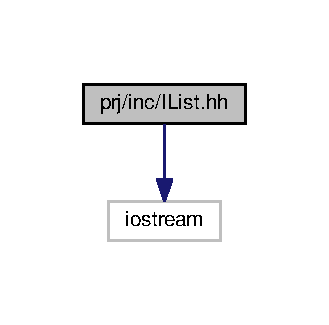
\includegraphics[width=158pt]{_i_list_8hh__incl}
\end{center}
\end{figure}
Ten wykres pokazuje, które pliki bezpośrednio lub pośrednio załączają ten plik\-:
\nopagebreak
\begin{figure}[H]
\begin{center}
\leavevmode
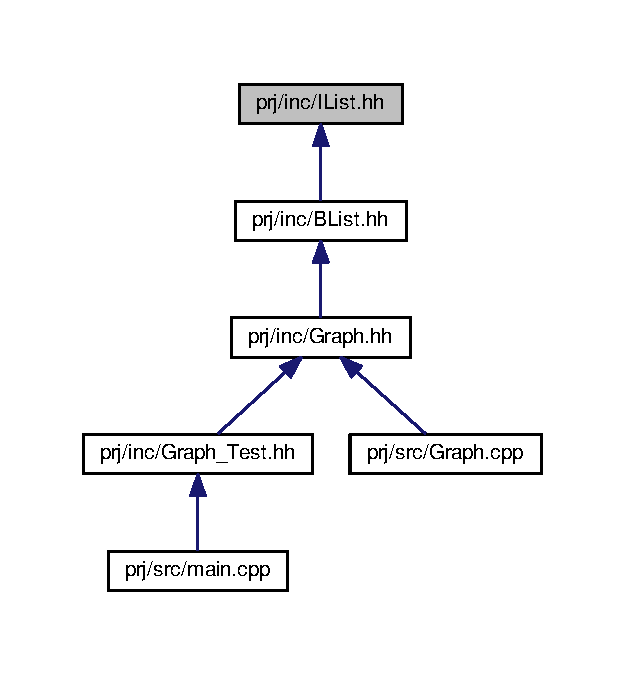
\includegraphics[width=300pt]{_i_list_8hh__dep__incl}
\end{center}
\end{figure}
\subsubsection*{Komponenty}
\begin{DoxyCompactItemize}
\item 
class \hyperlink{class_i_list}{I\-List$<$ Object $>$}
\begin{DoxyCompactList}\small\item\em Interfejs listy dwukierunkowej. \end{DoxyCompactList}\end{DoxyCompactItemize}


\subsubsection{Opis szczegółowy}
Plik zawiera interfejs listy dwukierunkową 

Definicja w pliku \hyperlink{_i_list_8hh_source}{I\-List.\-hh}.


\hypertarget{_i_queue_8hh}{\subsection{Dokumentacja pliku prj/inc/\-I\-Queue.hh}
\label{_i_queue_8hh}\index{prj/inc/\-I\-Queue.\-hh@{prj/inc/\-I\-Queue.\-hh}}
}
{\ttfamily \#include $<$iostream$>$}\\*
Wykres zależności załączania dla I\-Queue.\-hh\-:
\nopagebreak
\begin{figure}[H]
\begin{center}
\leavevmode
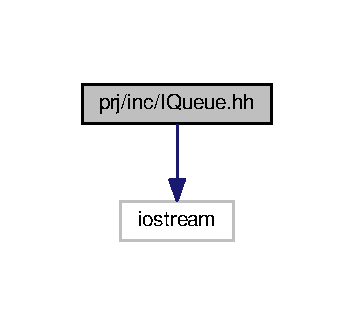
\includegraphics[width=170pt]{_i_queue_8hh__incl}
\end{center}
\end{figure}
Ten wykres pokazuje, które pliki bezpośrednio lub pośrednio załączają ten plik\-:
\nopagebreak
\begin{figure}[H]
\begin{center}
\leavevmode
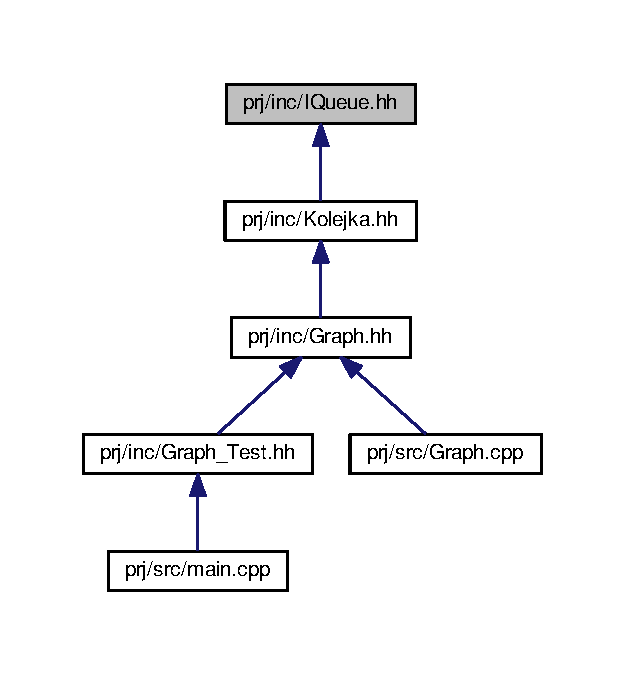
\includegraphics[width=300pt]{_i_queue_8hh__dep__incl}
\end{center}
\end{figure}
\subsubsection*{Komponenty}
\begin{DoxyCompactItemize}
\item 
class \hyperlink{class_i_queue}{I\-Queue$<$ Object $>$}
\begin{DoxyCompactList}\small\item\em Klasa modelująca interfejs kolejki. \end{DoxyCompactList}\end{DoxyCompactItemize}


\subsubsection{Opis szczegółowy}
Plik zawiera interfejs kolejki 

Definicja w pliku \hyperlink{_i_queue_8hh_source}{I\-Queue.\-hh}.


\hypertarget{_i_runnable_8hh}{\subsection{Dokumentacja pliku prj/inc/\-I\-Runnable.hh}
\label{_i_runnable_8hh}\index{prj/inc/\-I\-Runnable.\-hh@{prj/inc/\-I\-Runnable.\-hh}}
}
{\ttfamily \#include $<$iostream$>$}\\*
Wykres zależności załączania dla I\-Runnable.\-hh\-:
\nopagebreak
\begin{figure}[H]
\begin{center}
\leavevmode
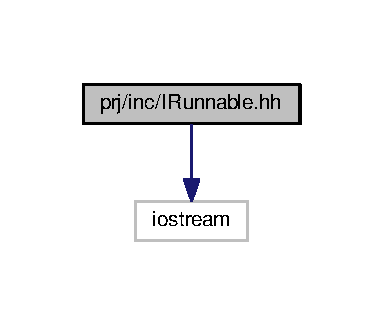
\includegraphics[width=184pt]{_i_runnable_8hh__incl}
\end{center}
\end{figure}
Ten wykres pokazuje, które pliki bezpośrednio lub pośrednio załączają ten plik\-:
\nopagebreak
\begin{figure}[H]
\begin{center}
\leavevmode
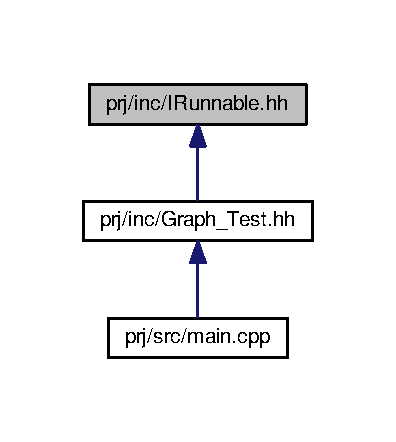
\includegraphics[width=190pt]{_i_runnable_8hh__dep__incl}
\end{center}
\end{figure}
\subsubsection*{Komponenty}
\begin{DoxyCompactItemize}
\item 
class \hyperlink{class_i_runnable}{I\-Runnable$<$ Object $>$}
\begin{DoxyCompactList}\small\item\em Klasa szablonowa modelująca interfejs \char`\"{}\-Biegacza\char`\"{}. \end{DoxyCompactList}\end{DoxyCompactItemize}


\subsubsection{Opis szczegółowy}
Plik zawiera interfejs obiektu, który można poddawać pomiarom czasu działania. 

Definicja w pliku \hyperlink{_i_runnable_8hh_source}{I\-Runnable.\-hh}.


\hypertarget{_i_stack_8hh}{\subsection{Dokumentacja pliku prj/inc/\-I\-Stack.hh}
\label{_i_stack_8hh}\index{prj/inc/\-I\-Stack.\-hh@{prj/inc/\-I\-Stack.\-hh}}
}
{\ttfamily \#include $<$iostream$>$}\\*
Wykres zależności załączania dla I\-Stack.\-hh\-:
\nopagebreak
\begin{figure}[H]
\begin{center}
\leavevmode
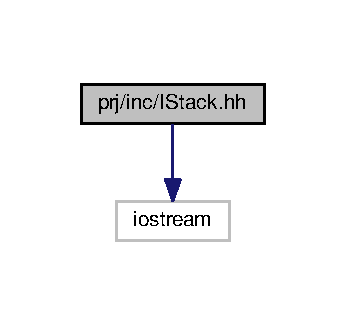
\includegraphics[width=166pt]{_i_stack_8hh__incl}
\end{center}
\end{figure}
Ten wykres pokazuje, które pliki bezpośrednio lub pośrednio załączają ten plik\-:
\nopagebreak
\begin{figure}[H]
\begin{center}
\leavevmode
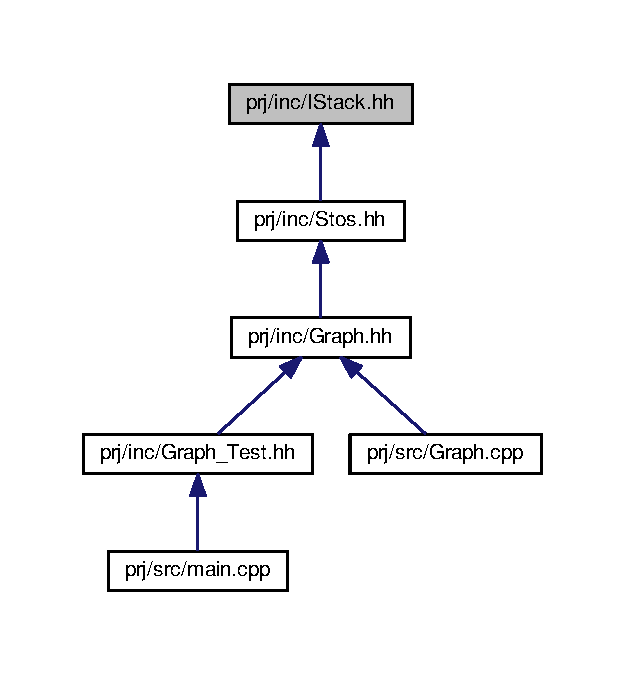
\includegraphics[width=300pt]{_i_stack_8hh__dep__incl}
\end{center}
\end{figure}
\subsubsection*{Komponenty}
\begin{DoxyCompactItemize}
\item 
class \hyperlink{class_i_stack}{I\-Stack$<$ Object $>$}
\begin{DoxyCompactList}\small\item\em Klasa szablonowa modelująca interfejs stosu. \end{DoxyCompactList}\end{DoxyCompactItemize}


\subsubsection{Opis szczegółowy}
Plik zawiera interfejs stosu 

Definicja w pliku \hyperlink{_i_stack_8hh_source}{I\-Stack.\-hh}.


\hypertarget{_kolejka_8hh}{\subsection{Dokumentacja pliku prj/inc/\-Kolejka.hh}
\label{_kolejka_8hh}\index{prj/inc/\-Kolejka.\-hh@{prj/inc/\-Kolejka.\-hh}}
}
{\ttfamily \#include $<$iostream$>$}\\*
{\ttfamily \#include \char`\"{}I\-Queue.\-hh\char`\"{}}\\*
{\ttfamily \#include \char`\"{}S\-Node.\-hh\char`\"{}}\\*
Wykres zależności załączania dla Kolejka.\-hh\-:
\nopagebreak
\begin{figure}[H]
\begin{center}
\leavevmode
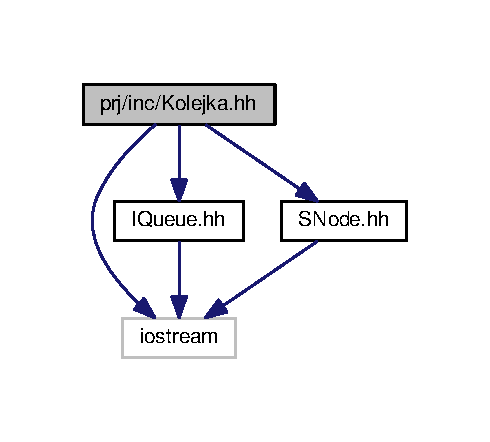
\includegraphics[width=235pt]{_kolejka_8hh__incl}
\end{center}
\end{figure}
Ten wykres pokazuje, które pliki bezpośrednio lub pośrednio załączają ten plik\-:
\nopagebreak
\begin{figure}[H]
\begin{center}
\leavevmode
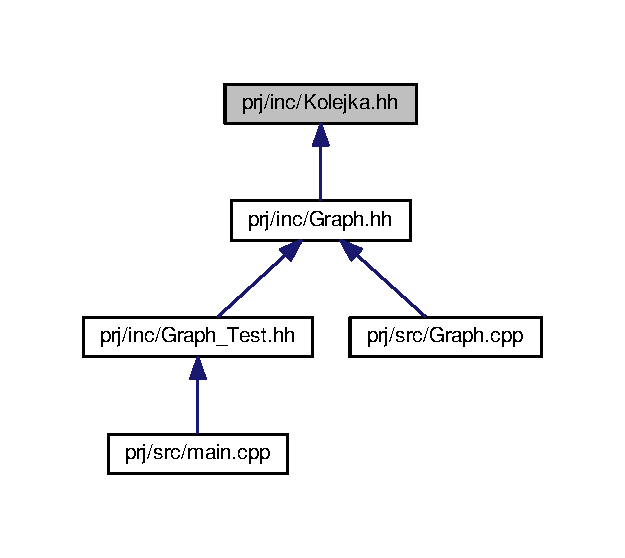
\includegraphics[width=300pt]{_kolejka_8hh__dep__incl}
\end{center}
\end{figure}
\subsubsection*{Komponenty}
\begin{DoxyCompactItemize}
\item 
class \hyperlink{class_kolejka}{Kolejka$<$ Object $>$}
\begin{DoxyCompactList}\small\item\em Klasa szablonowa implementująca kolejkę \end{DoxyCompactList}\end{DoxyCompactItemize}


\subsubsection{Opis szczegółowy}
Plik zawiera implementację interfejsu kolejki 

Definicja w pliku \hyperlink{_kolejka_8hh_source}{Kolejka.\-hh}.


\hypertarget{_s_node_8hh}{\subsection{Dokumentacja pliku prj/inc/\-S\-Node.hh}
\label{_s_node_8hh}\index{prj/inc/\-S\-Node.\-hh@{prj/inc/\-S\-Node.\-hh}}
}
{\ttfamily \#include $<$iostream$>$}\\*
Wykres zależności załączania dla S\-Node.\-hh\-:
\nopagebreak
\begin{figure}[H]
\begin{center}
\leavevmode
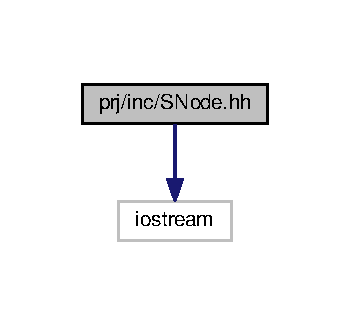
\includegraphics[width=168pt]{_s_node_8hh__incl}
\end{center}
\end{figure}
Ten wykres pokazuje, które pliki bezpośrednio lub pośrednio załączają ten plik\-:
\nopagebreak
\begin{figure}[H]
\begin{center}
\leavevmode
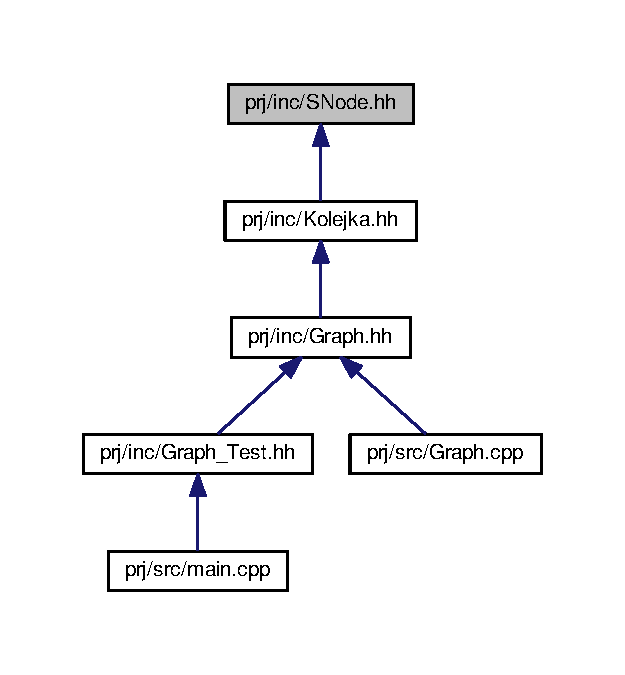
\includegraphics[width=300pt]{_s_node_8hh__dep__incl}
\end{center}
\end{figure}
\subsubsection*{Komponenty}
\begin{DoxyCompactItemize}
\item 
class \hyperlink{class_s_node}{S\-Node$<$ Object $>$}
\end{DoxyCompactItemize}

\hypertarget{_stopwatch_8hh}{\subsection{Dokumentacja pliku prj/inc/\-Stopwatch.hh}
\label{_stopwatch_8hh}\index{prj/inc/\-Stopwatch.\-hh@{prj/inc/\-Stopwatch.\-hh}}
}
{\ttfamily \#include $<$iostream$>$}\\*
{\ttfamily \#include $<$ctime$>$}\\*
{\ttfamily \#include $<$sys/time.\-h$>$}\\*
Wykres zależności załączania dla Stopwatch.\-hh\-:
\nopagebreak
\begin{figure}[H]
\begin{center}
\leavevmode
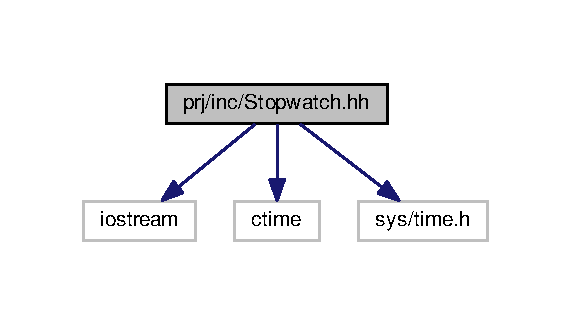
\includegraphics[width=274pt]{_stopwatch_8hh__incl}
\end{center}
\end{figure}
Ten wykres pokazuje, które pliki bezpośrednio lub pośrednio załączają ten plik\-:
\nopagebreak
\begin{figure}[H]
\begin{center}
\leavevmode
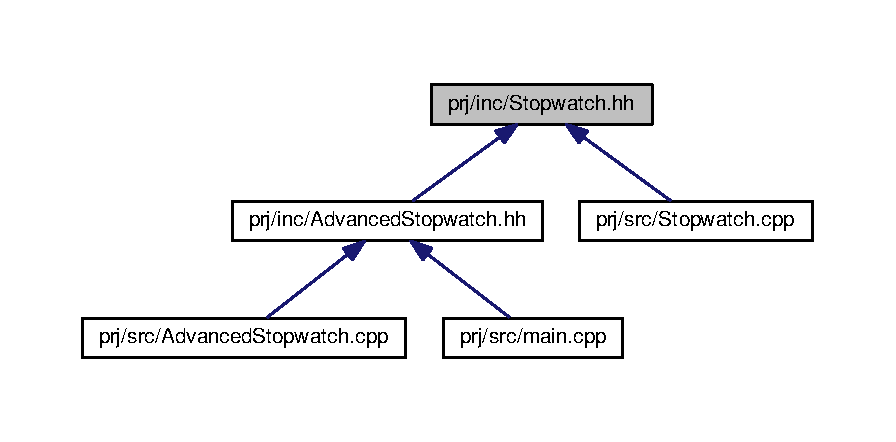
\includegraphics[width=350pt]{_stopwatch_8hh__dep__incl}
\end{center}
\end{figure}
\subsubsection*{Komponenty}
\begin{DoxyCompactItemize}
\item 
class \hyperlink{class_stopwatch}{Stopwatch}
\begin{DoxyCompactList}\small\item\em Klasa implementująca podstawowy stoper. \end{DoxyCompactList}\end{DoxyCompactItemize}


\subsubsection{Opis szczegółowy}
Plik zawiera implementację podstawowego stopera. 

Definicja w pliku \hyperlink{_stopwatch_8hh_source}{Stopwatch.\-hh}.


\hypertarget{_stos_8hh}{\subsection{Dokumentacja pliku prj/inc/\-Stos.hh}
\label{_stos_8hh}\index{prj/inc/\-Stos.\-hh@{prj/inc/\-Stos.\-hh}}
}
{\ttfamily \#include \char`\"{}I\-Stack.\-hh\char`\"{}}\\*
Wykres zależności załączania dla Stos.\-hh\-:
\nopagebreak
\begin{figure}[H]
\begin{center}
\leavevmode
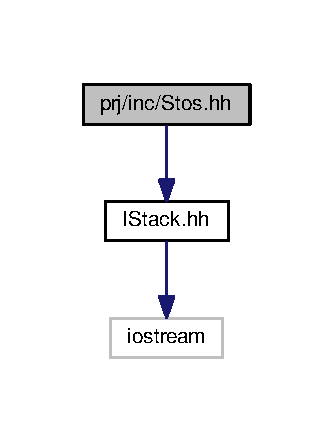
\includegraphics[width=160pt]{_stos_8hh__incl}
\end{center}
\end{figure}
Ten wykres pokazuje, które pliki bezpośrednio lub pośrednio załączają ten plik\-:
\nopagebreak
\begin{figure}[H]
\begin{center}
\leavevmode
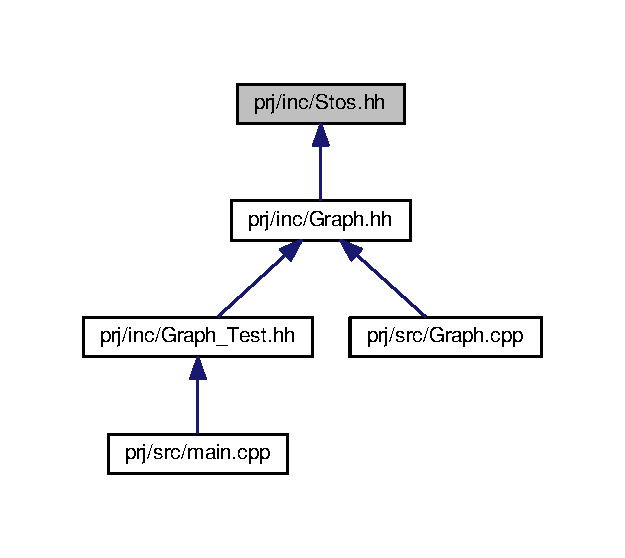
\includegraphics[width=300pt]{_stos_8hh__dep__incl}
\end{center}
\end{figure}
\subsubsection*{Komponenty}
\begin{DoxyCompactItemize}
\item 
class \hyperlink{class_stos}{Stos$<$ Object $>$}
\begin{DoxyCompactList}\small\item\em Klasa szablonowa implementująca stos. \end{DoxyCompactList}\end{DoxyCompactItemize}


\subsubsection{Opis szczegółowy}
Plik zawiera implementację interfejsu stosu 

Definicja w pliku \hyperlink{_stos_8hh_source}{Stos.\-hh}.


\hypertarget{_advanced_stopwatch_8cpp}{\subsection{Dokumentacja pliku prj/src/\-Advanced\-Stopwatch.cpp}
\label{_advanced_stopwatch_8cpp}\index{prj/src/\-Advanced\-Stopwatch.\-cpp@{prj/src/\-Advanced\-Stopwatch.\-cpp}}
}
{\ttfamily \#include \char`\"{}Advanced\-Stopwatch.\-hh\char`\"{}}\\*
Wykres zależności załączania dla Advanced\-Stopwatch.\-cpp\-:
\nopagebreak
\begin{figure}[H]
\begin{center}
\leavevmode
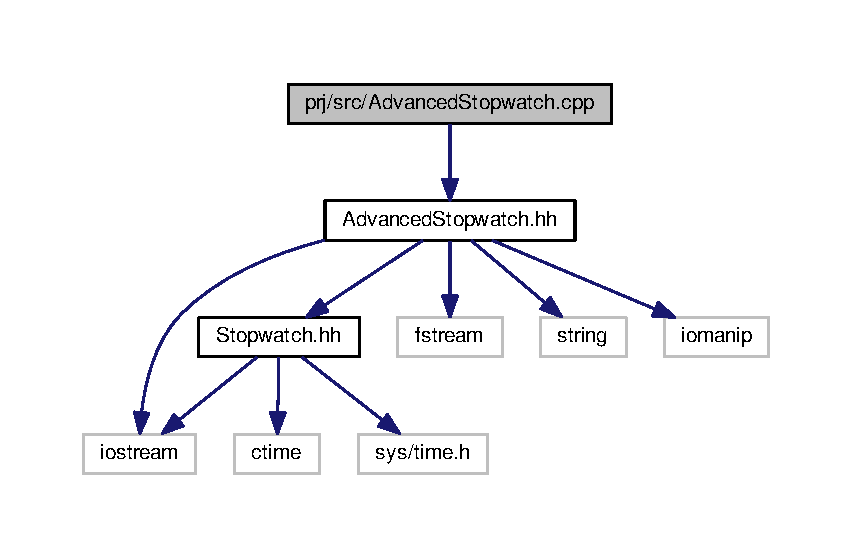
\includegraphics[width=350pt]{_advanced_stopwatch_8cpp__incl}
\end{center}
\end{figure}

\hypertarget{_graph_8cpp}{\subsection{Dokumentacja pliku prj/src/\-Graph.cpp}
\label{_graph_8cpp}\index{prj/src/\-Graph.\-cpp@{prj/src/\-Graph.\-cpp}}
}
{\ttfamily \#include \char`\"{}Graph.\-hh\char`\"{}}\\*
Wykres zależności załączania dla Graph.\-cpp\-:
\nopagebreak
\begin{figure}[H]
\begin{center}
\leavevmode
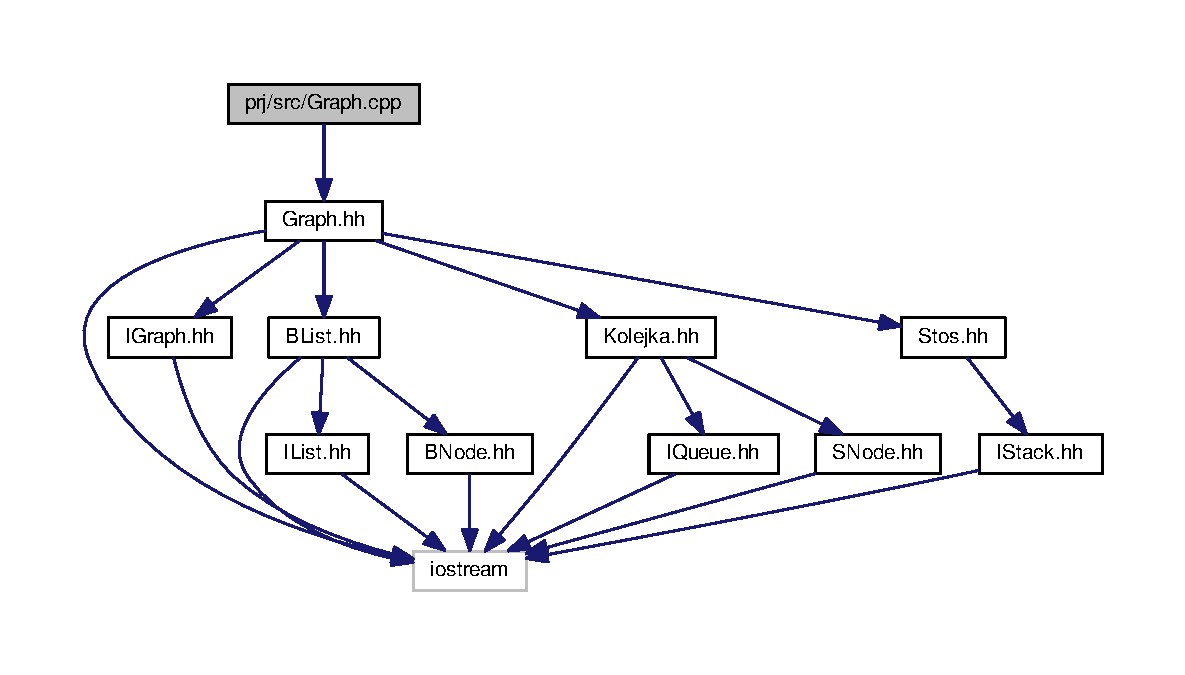
\includegraphics[width=350pt]{_graph_8cpp__incl}
\end{center}
\end{figure}

\hypertarget{main_8cpp}{\subsection{Dokumentacja pliku prj/src/main.cpp}
\label{main_8cpp}\index{prj/src/main.\-cpp@{prj/src/main.\-cpp}}
}
{\ttfamily \#include $<$iostream$>$}\\*
{\ttfamily \#include \char`\"{}Graph\-\_\-\-Test.\-hh\char`\"{}}\\*
{\ttfamily \#include \char`\"{}Advanced\-Stopwatch.\-hh\char`\"{}}\\*
Wykres zależności załączania dla main.\-cpp\-:
\nopagebreak
\begin{figure}[H]
\begin{center}
\leavevmode
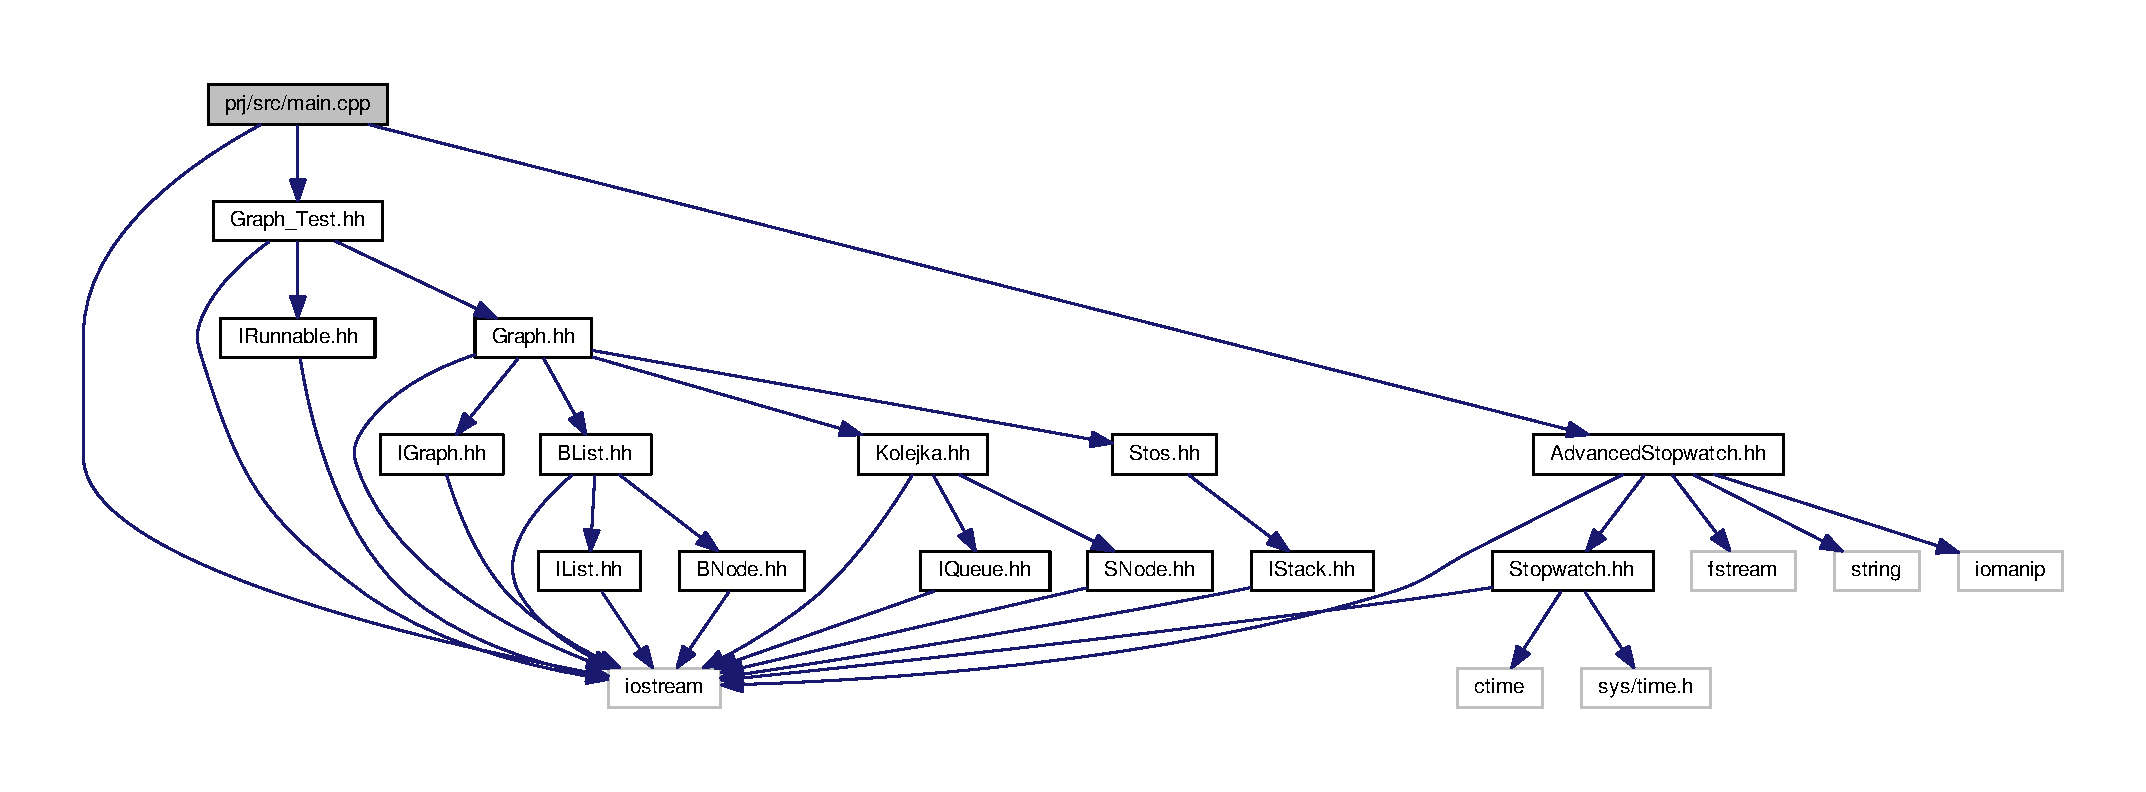
\includegraphics[width=350pt]{main_8cpp__incl}
\end{center}
\end{figure}
\subsubsection*{Funkcje}
\begin{DoxyCompactItemize}
\item 
int \hyperlink{main_8cpp_ae66f6b31b5ad750f1fe042a706a4e3d4}{main} ()
\end{DoxyCompactItemize}


\subsubsection{Dokumentacja funkcji}
\hypertarget{main_8cpp_ae66f6b31b5ad750f1fe042a706a4e3d4}{\index{main.\-cpp@{main.\-cpp}!main@{main}}
\index{main@{main}!main.cpp@{main.\-cpp}}
\paragraph[{main}]{\setlength{\rightskip}{0pt plus 5cm}int main (
\begin{DoxyParamCaption}
{}
\end{DoxyParamCaption}
)}}\label{main_8cpp_ae66f6b31b5ad750f1fe042a706a4e3d4}


Definicja w linii 7 pliku main.\-cpp.


\hypertarget{_stopwatch_8cpp}{\subsection{Dokumentacja pliku prj/src/\-Stopwatch.cpp}
\label{_stopwatch_8cpp}\index{prj/src/\-Stopwatch.\-cpp@{prj/src/\-Stopwatch.\-cpp}}
}
{\ttfamily \#include \char`\"{}Stopwatch.\-hh\char`\"{}}\\*
Wykres zależności załączania dla Stopwatch.\-cpp\-:
\nopagebreak
\begin{figure}[H]
\begin{center}
\leavevmode
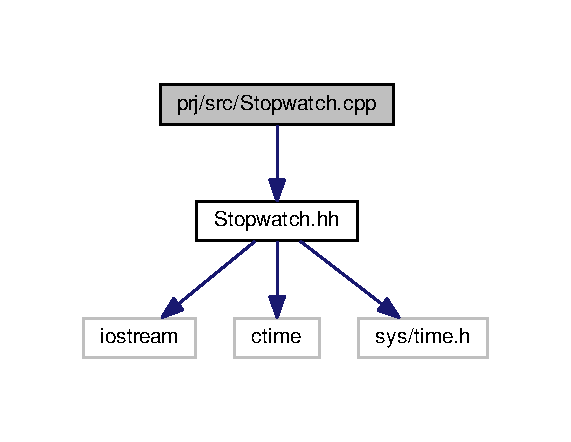
\includegraphics[width=274pt]{_stopwatch_8cpp__incl}
\end{center}
\end{figure}

%--- End generated contents ---

% Index
\newpage
\phantomsection
\addcontentsline{toc}{section}{Indeks}
\printindex

\end{document}
